\section{Overview}%
\label{sec:chap4Overview}
\autoBookmark{sec}{Overview}
This chapter reports the results of the demonstration and evaluation activities, Activities~4 and~5 in \reff{fig:dsrm_flow}. The results follow the workflow of \reff{fig:methodology_framework}, so that each stage of the pipeline is evaluated at the point where it acts on the data, and each result is given first for the primary Tomasov dataset and then for the Cao evaluation dataset.

The chapter answers the three research questions. \refs{sec:resLeakage} first reports the leakage audit of the released protocols and the verified partitions that replace them, which form the evaluation basis for all subsequent results. For RQ2, the development of the pipeline, \refs{sec:resDomains} evaluates multi-domain fusion, \refs{sec:resSelection} consensus feature selection and its effect on the footprint, \refs{sec:resBalancing} class balancing, and \refs{sec:resFinal} the choice of classifier, with the pipeline developed on Tomasov applied unchanged to Cao. For RQ1, the lightweight footprint, \refs{sec:resEfficiency} measures the model size, latency, and training cost of the pipeline and of every baseline on the same embedded platform. For RQ3, the evaluation, \refs{sec:resPerformance} and \refs{sec:resStats} examine per-class behaviour and test whether the observed differences exceed the variation expected from the data. \refs{sec:resConfound}, \refs{sec:resGeneralisationAll}, and \refs{sec:resMapping} examine the extent to which performance generalises beyond the recordings and the system on which the pipeline was trained, the last through a mapping between the two event taxonomies. \refs{sec:resDiscussion} compares the pipeline with the CNN published with each dataset and with five recent architectures on identical partitions, measures the extent to which the partition alone changes the score of a model, and contrasts the white-box character of the pipeline with the black-box character of the deep baselines.

\section{Datasets and Leakage Assessment}
\label{sec:resLeakage}
\autoBookmark{sec}{Datasets and Leakage Assessment}
Every subsequent result depends on the first stages of \reff{fig:methodology_framework}, in which both datasets undergo the leakage audit, group-aware partitioning, and class decimation. Before any model was trained, the audit of \refss{sec:chap3LeakageAudit} was applied to each dataset and its released protocol. The audit examined whether overlapping windows allow raw samples to be shared between the training and test data, and whether recording sessions contribute to both. Both questions are important because a score measured on dependent partitions may reflect the recognition of a recording, or of signal already encountered in training, rather than generalisation to new event instances.

\subsection{Leakage in the Tomasov Protocol}
\label{sec:resLeakageTomasov}
\autoBookmark{subsec}{Leakage in the Tomasov Protocol}
A reconstruction of the raw-sample blocks read by each split under a random stratified $80/10/10$ partition shows that $43{,}976$ of $43{,}976$ test windows ($100.0\%$) share raw samples with at least one training window. Under a random partition, every test window thus has a corresponding training window that contains part of its raw signal, and test accuracy measures the recognition of previously observed signal as much as the recognition of events. Under the blocked partition with guard bands the same measurement returns $0$ of $31{,}028$ ($0.0\%$).

\subsection{Leakage in the Released Cao Partition}
\label{sec:resLeakageCao}
\autoBookmark{subsec}{Leakage in the Released Cao Partition}
Of the 441 recording sessions recovered from the Cao filenames, 423 ($95.9\%$) contribute records to both the released training and test folders, and only 18 are confined to a single folder. Almost the entire released test set is therefore drawn from sessions that the model has already encountered in training, and accuracies measured on it, including those of the SVM and CNN baselines distributed with the dataset, consequently reflect within-recording recognition as much as event recognition. Table~\ref{tab:leakage_audit} summarises both audits.

\begin{table}[!htbp]
	\centering
	\caption{Leakage assessment of the released and leakage-controlled evaluation protocols.}
	\label{tab:leakage_audit}
	\small
	\resizebox{\textwidth}{!}{%
\begin{tabular}{@{}llr@{}}
		\toprule
		\textbf{Dataset / protocol} & \textbf{Contamination measure} & \textbf{Value}\\
		\midrule
		Tomasov, random 80/10/10          & Test windows sharing raw samples with training & $100.0\%$\\
		Tomasov, blocked + guard (proposed) & Test windows sharing raw samples with training & $0.0\%$\\
		\midrule
		Cao, released 8:2                 & Sessions spanning train and test & 423 / 441\\
		Cao, session-grouped (proposed)   & Sessions spanning train and test & 0 / 441\\
		\bottomrule
	\end{tabular}}
\end{table}

\subsection{Class-Balance Decimation and Group-Aware Split}
\label{sec:resDecimationSplit}
\autoBookmark{subsec}{Class-Balance Decimation and Group-Aware Split}
The group-aware split and the class-balance decimation of \reff{fig:methodology_framework} together determine the populations on which every subsequent result is computed. For Tomasov, the two test populations quoted in this thesis, $31{,}028$ in \refs{sec:resLeakageTomasov} and $11{,}334$ in Table~\ref{tab:split_summary}, are two stages of a single partition rather than two partitions. The audit is performed immediately after blocked assignment and guard-band removal, because that is the stage at which sample disjointness is established. Class decimation, which caps the three most populous classes so that none dominates training, follows and removes a further $19{,}694$ test windows ($63.5\%$), leaving the $11{,}334$ on which every reported result is computed. Decimation deletes whole windows and can only reduce the raw-sample footprint of the test set; the verification was nonetheless repeated on the final test set, and none of its $11{,}334$ windows shares a raw sample with any training window. For Cao, the session-grouped split places each of the 441 sessions in exactly one split, so no session contributes to both training and test (Table~\ref{tab:leakage_audit}).

These measurements explain why several results in this chapter are lower than previously published values for the same benchmarks. A lower score in this chapter does not in itself indicate a weaker method; it reflects the same class of method measured under a protocol that is free of contamination. The verified partitions are the evaluation basis for every accuracy reported under RQ2 and RQ3 and for the training times of RQ1, and the protocol-attribution experiments of \refs{sec:resDiscussion} quantify the effect of leakage on reported accuracy.

\section{Multi-Domain Feature Extraction and Fusion}
\label{sec:resDomains}
\autoBookmark{sec}{Multi-Domain Feature Extraction and Fusion}
The extraction stage of \reff{fig:methodology_framework} produces four domain-specific feature sets, which the feature-vector construction step concatenates into a single $1{,}002$-dimensional representation. Table~\ref{tab:domain_comparison} reports the best configuration for each individual domain and for the fused representation, each selected from the same reduced search space so that the feature set is the only variable. Fusion yields the highest performance on both datasets, exceeding the best single domain by $6.26$ macro-$F_1$ points on Tomasov and $3.46$ on Cao. The four domains therefore carry complementary information, which answers the first part of \textbf{RQ2}. Because this search space is restricted rather than exhaustive, the fused values differ from the headline results of Table~\ref{tab:main_results} by $0.16$ and $0.01$ points; the domain ordering is unaffected.

\begin{table}[H]
	\centering
	\caption{Best configuration by feature domain (test macro-$F_1$, \%), selected from a common reduced search space and ordered as in the feature-extraction sequence of Chapter~\ref{chap:methodology}.}
	\label{tab:domain_comparison}
	\small
	\begin{tabular*}{\textwidth}{@{\extracolsep{\fill}}lrrrl@{}}
		\toprule
		\textbf{Domain} & \textbf{Features} & \textbf{Tomasov} & \textbf{Cao} & \textbf{Reference}\\
		\midrule
		Time              & 112     & 54.82          & 90.69          & Table~\ref{tab:timefeatures}\\
		Frequency         & 90      & 55.23          & 79.51          & Table~\ref{tab:freqfeatures}\\
		Time--frequency   & 739     & 58.98          & 92.51          & Table~\ref{tab:tffeatures}\\
		Spatial           & 61      & 75.56          & 95.42          & Table~\ref{tab:spatialfeatures}\\
		\bottomrule
		Multi-domain      & 1{,}002 & \textbf{81.82} & \textbf{98.89} & Table~\ref{tab:dimensionality}\\
		\bottomrule
	\end{tabular*}
\end{table}

The domain ordering is almost identical on the two systems, with a Spearman rank correlation of $\rho = 0.90$ (\reff{fig:domain_agreement}). Because the two acquisitions share no hardware or taxonomy, this agreement suggests that the relative value of the representations is a property of the method rather than of a single site. One result, however, is contrary to expectation. The spatial domain is the strongest single domain on both datasets, and on Tomasov its 61 features outperform the 739 time--frequency features by $16.58$ points. \refs{sec:resConfound} therefore examines the extent to which this result reflects recording-specific structure rather than event information.

\begin{figure}[!htbp]
\centering
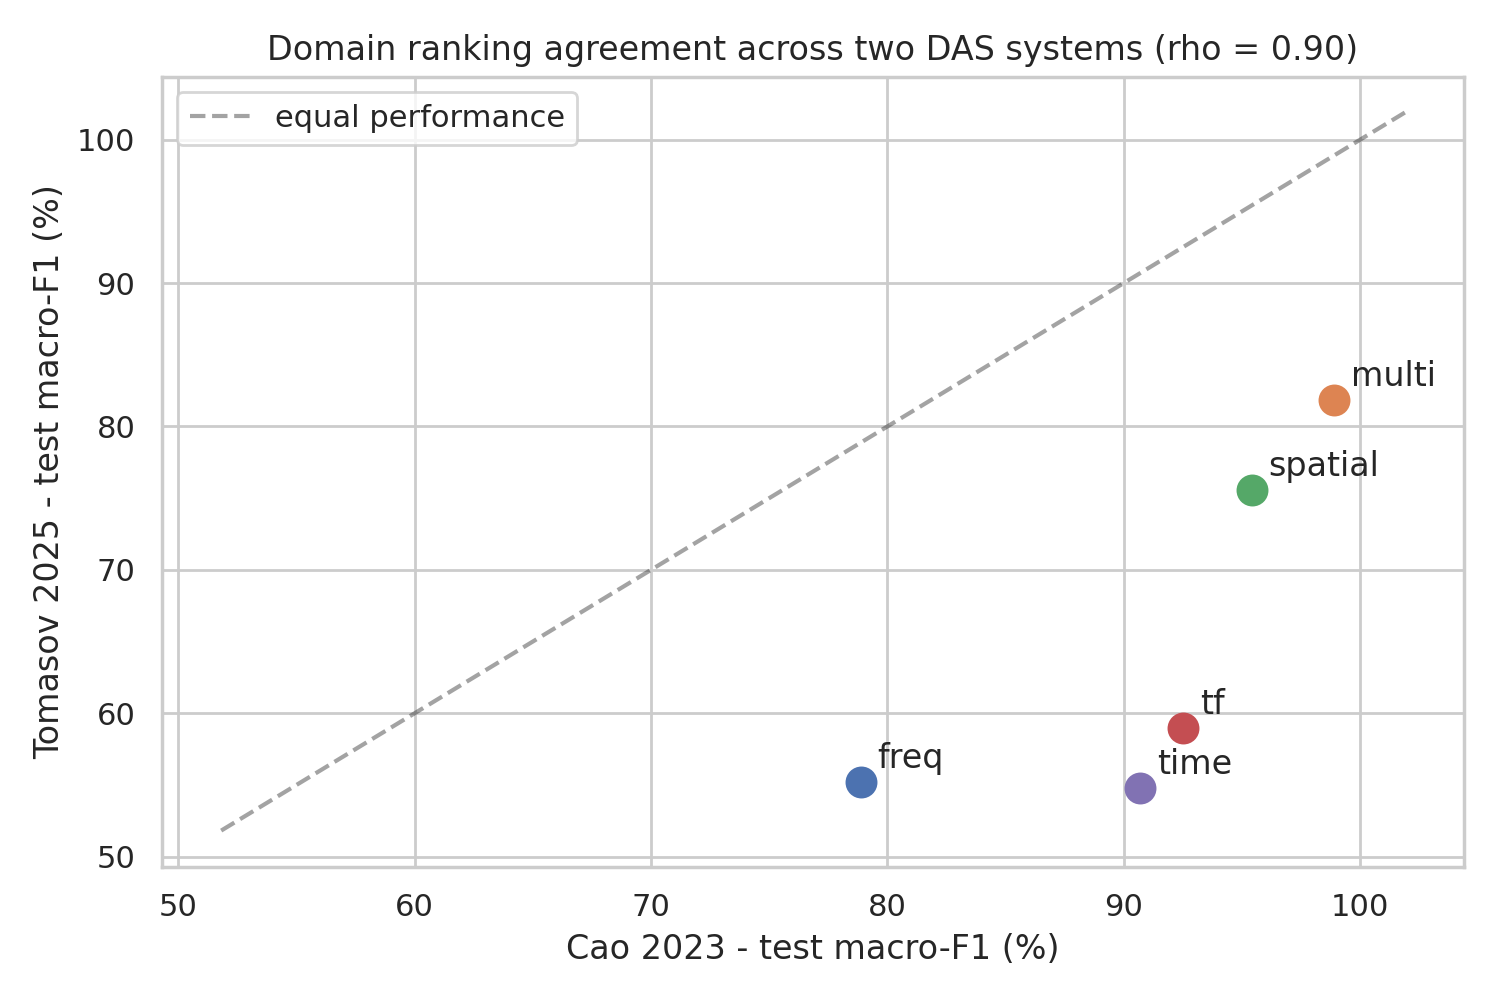
\includegraphics[width=0.75\textwidth,keepaspectratio]{Figures/fig24_domain_agreement.png}
\caption{Agreement in feature-domain performance across the two DAS systems ($\rho = 0.90$).}
\label{fig:domain_agreement}
\end{figure}

\section{Feature Selection}
\label{sec:resSelection}
\autoBookmark{sec}{Feature Selection}
After the group-aware split, \reff{fig:methodology_framework} branches on the feature set: models are trained either on the full fused vector or on the subset retained by the eight-method ensemble, which is fitted on the training set only. The requirement that all eight selectors agree produces compact subsets of 52 of the $1{,}002$ features on Tomasov and 53 on Cao, reductions of $94.8\%$ and $94.7\%$. \reff{fig:consensus_votes} shows the vote distribution on Tomasov and the domain composition of the retained set, and Table~\ref{tab:consensus} gives the composition for both datasets. Time--frequency descriptors constitute $67\%$ and $72\%$ of the two subsets even though that domain is not the strongest in isolation, which indicates that its contribution is complementary rather than redundant.

\begin{figure}[!htbp]
\centering
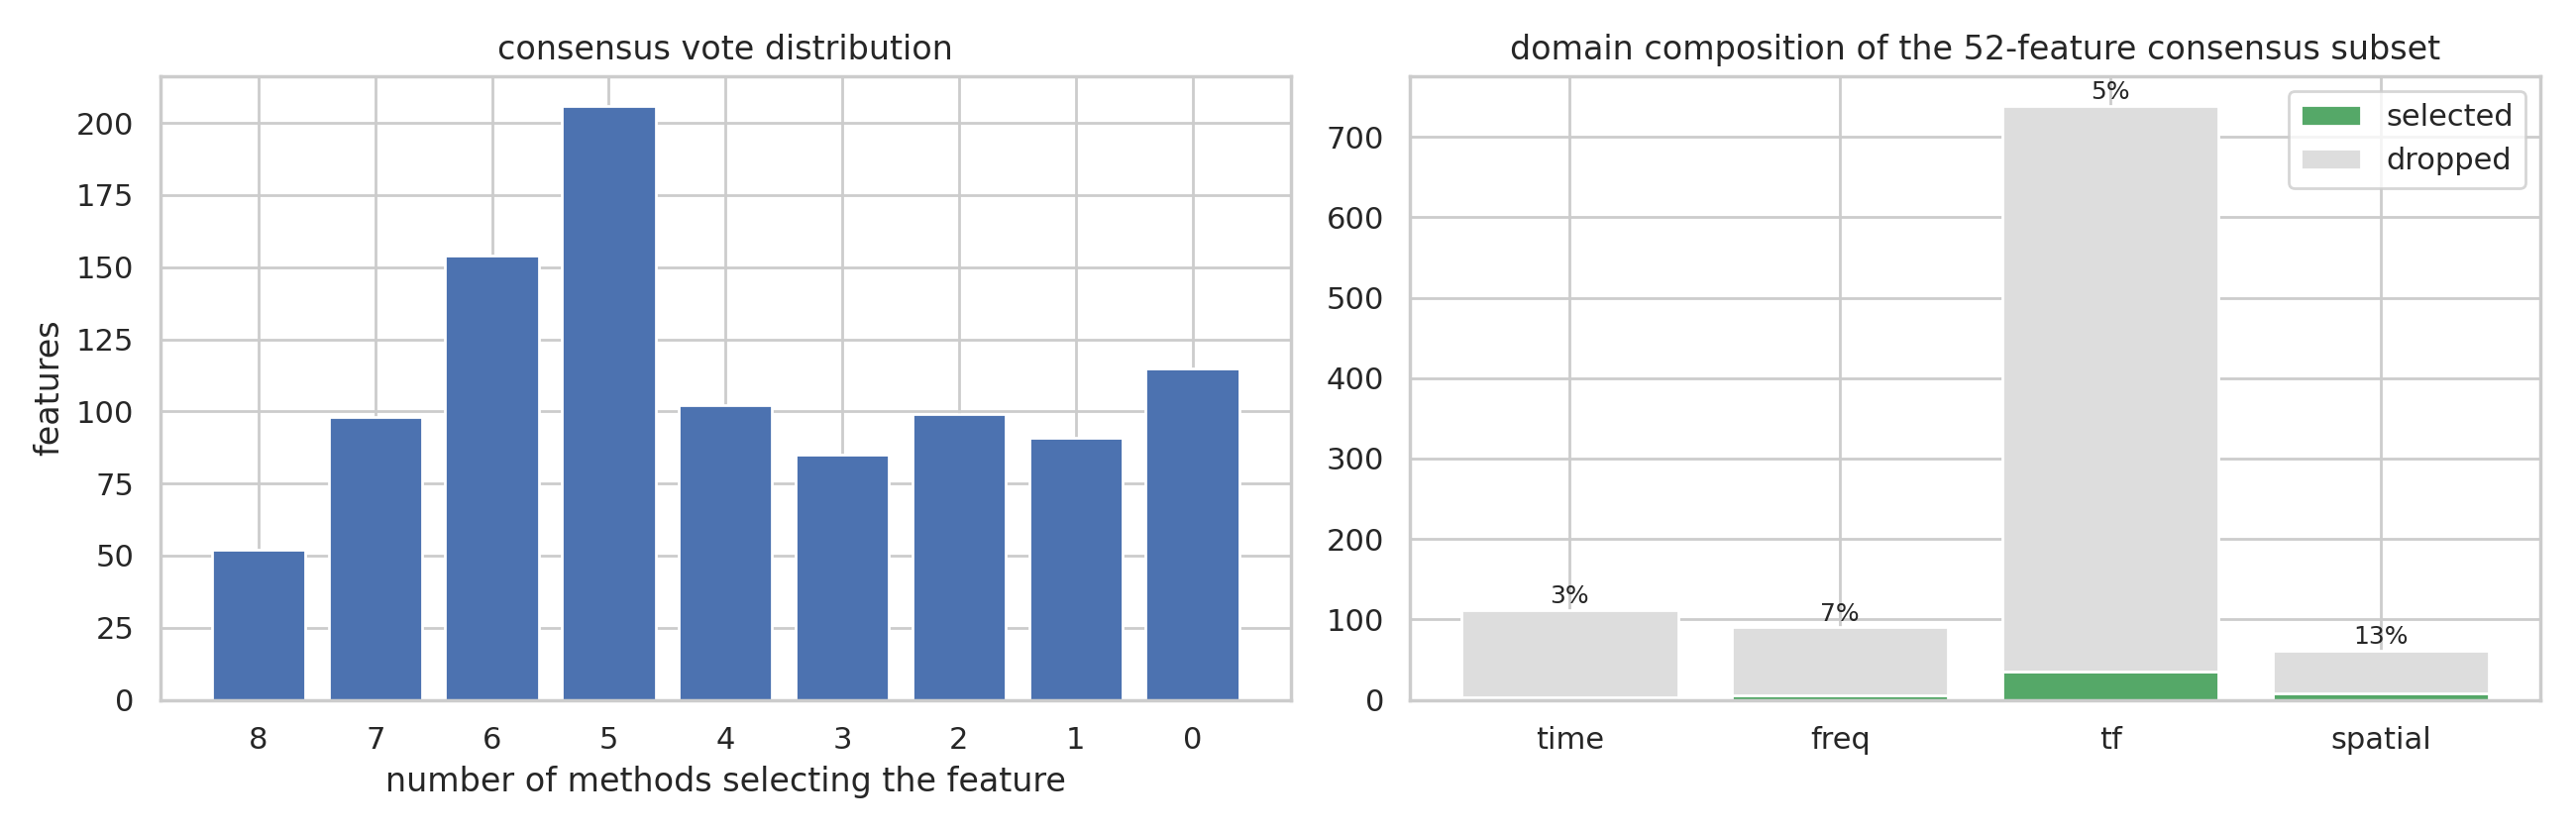
\includegraphics[width=0.95\textwidth,keepaspectratio]{Figures/fig30_consensus_votes_tomasov.png}
\caption{Consensus voting on the Tomasov dataset: number of features selected by $k$ of the eight methods (left) and the domain composition of the 52-feature unanimous subset (right).}
\label{fig:consensus_votes}
\end{figure}

\begin{table}[H]
	\centering
	\caption{Domain composition of the unanimous consensus subsets. Retained is the percentage of that domain's features kept.}
	\label{tab:consensus}
	\small
	\begin{tabular}{@{}lrrrr@{}}
		\toprule
		& \multicolumn{2}{c}{\textbf{Tomasov}} & \multicolumn{2}{c}{\textbf{Cao}}\\
		\cmidrule(lr){2-3}\cmidrule(lr){4-5}
		\textbf{Domain} & \textbf{Selected} & \textbf{Retained} & \textbf{Selected} & \textbf{Retained}\\
		\midrule
		Time            & 3  & 2.7\%  & 12 & 10.7\%\\
		Frequency       & 6  & 6.7\%  & 2  & 2.2\%\\
		Time--frequency & 35 & 4.7\%  & 38 & 5.1\%\\
		Spatial         & 8  & 13.1\% & 1  & 1.6\%\\
		\midrule
		\textbf{Total}  & \textbf{52} & \textbf{5.2\%} & \textbf{53} & \textbf{5.3\%}\\
		\bottomrule
	\end{tabular}
\end{table}

\reff{fig:jaccard} shows the pairwise Jaccard agreement between selectors. Agreement is moderate, and the variance threshold overlaps least with the relevance-based methods, as expected of an unsupervised criterion. This diversity is what makes the unanimity rule meaningful: a feature retained by all eight selectors has simultaneous support from linear correlation, information content, neighbourhood separability, redundancy penalisation, tree importance, and model attribution.

\begin{figure}[!htbp]
\centering
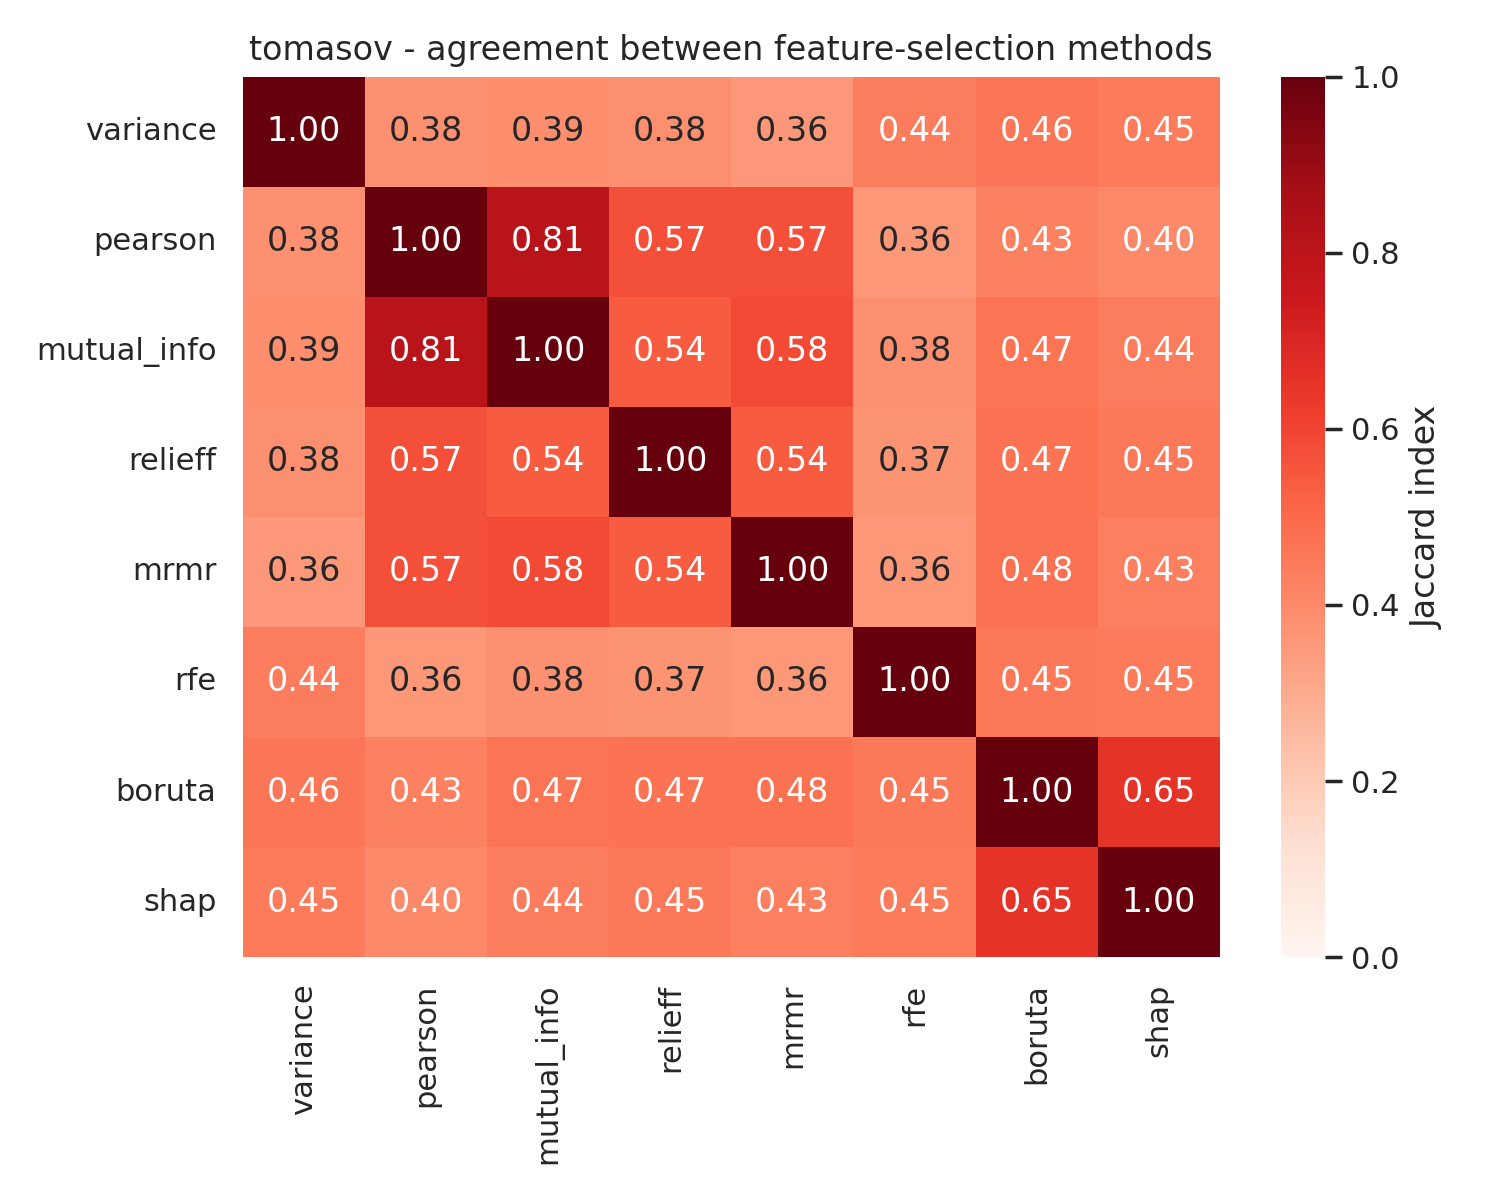
\includegraphics[width=0.48\textwidth,keepaspectratio]{Figures/fig16a_jaccard_tomasov.png}
\hfill
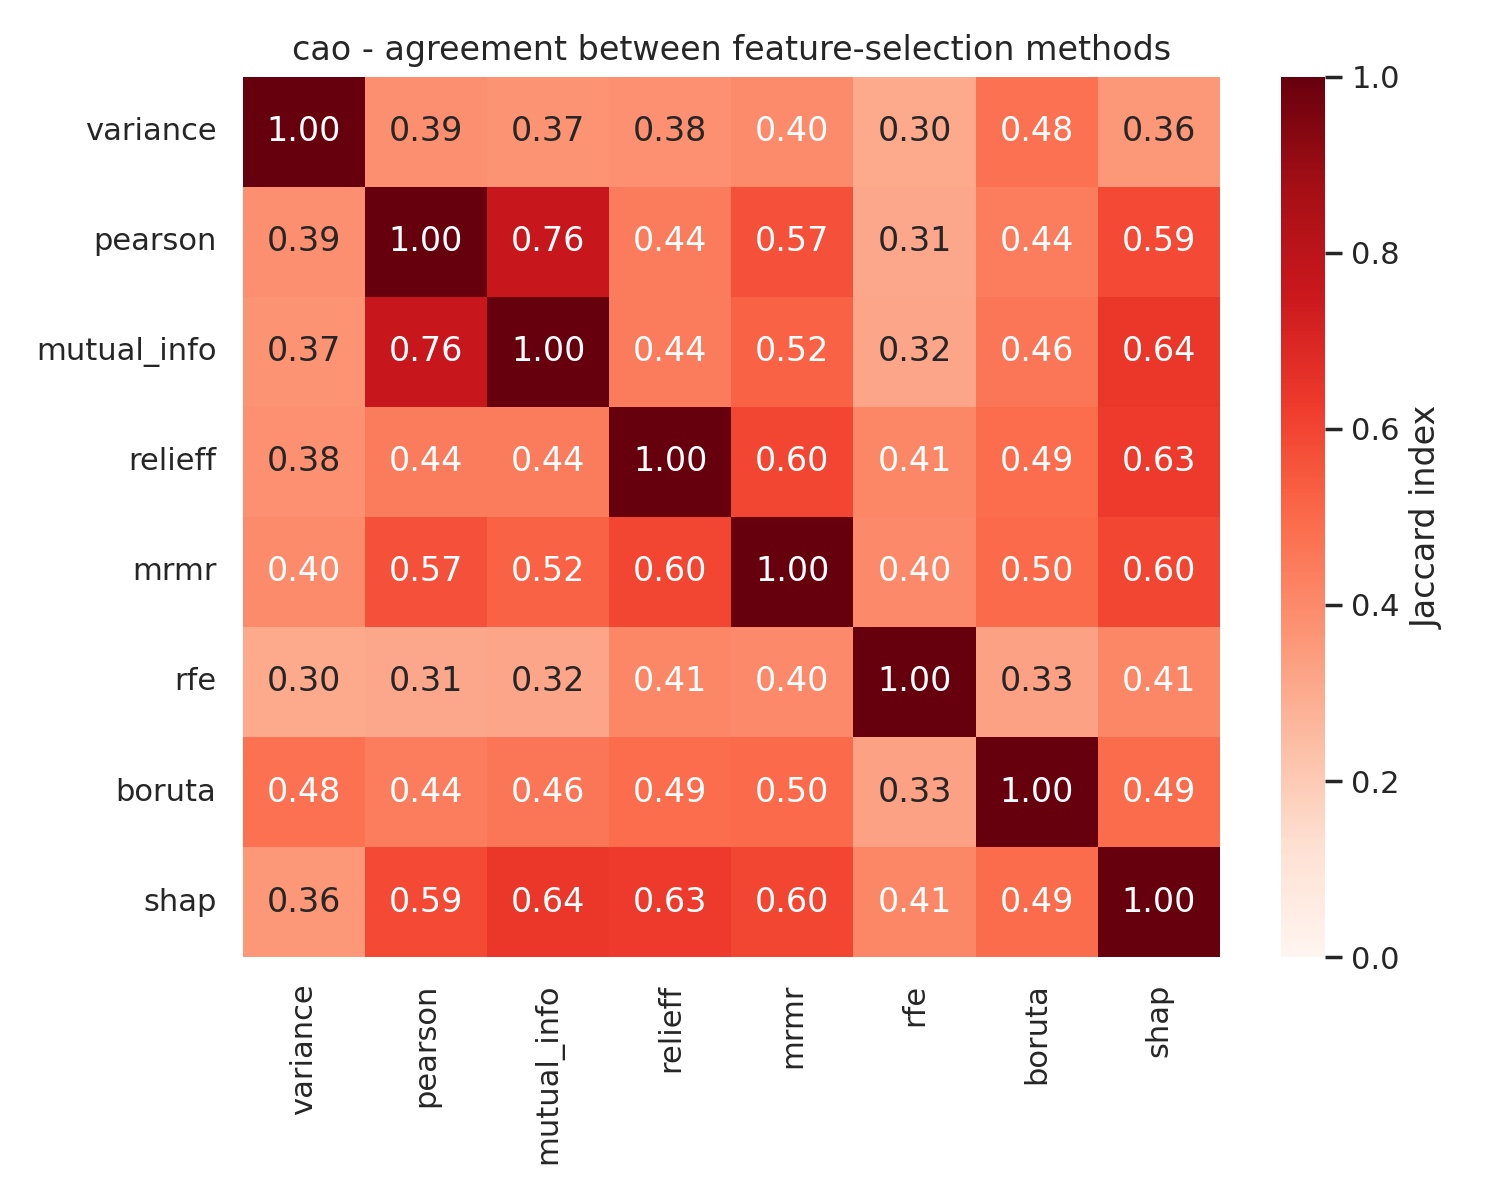
\includegraphics[width=0.48\textwidth,keepaspectratio]{Figures/fig16b_jaccard_cao.png}
\caption{Pairwise Jaccard agreement between the eight feature-selection methods: Tomasov (left) and Cao (right).}
\label{fig:jaccard}
\end{figure}

Compactness is obtained at a cost in accuracy. \reff{fig:reduction} plots validation performance against the number of retained features: the consensus subsets reduce macro-$F_1$ by $8.39$ points on Tomasov ($81.98$ to $73.59$) and by $5.81$ on Cao ($98.90$ to $93.08$). These losses are considerably larger than the sub-point penalty reported in earlier single-dataset work on this benchmark, and they alter the practical recommendation. Unanimous consensus is appropriate when efficiency or interpretability requirements are stringent; otherwise an intermediate operating point on the reduction curve is preferable. This finding answers the feature-selection part of \textbf{RQ2}.

\begin{figure}[!htbp]
\centering
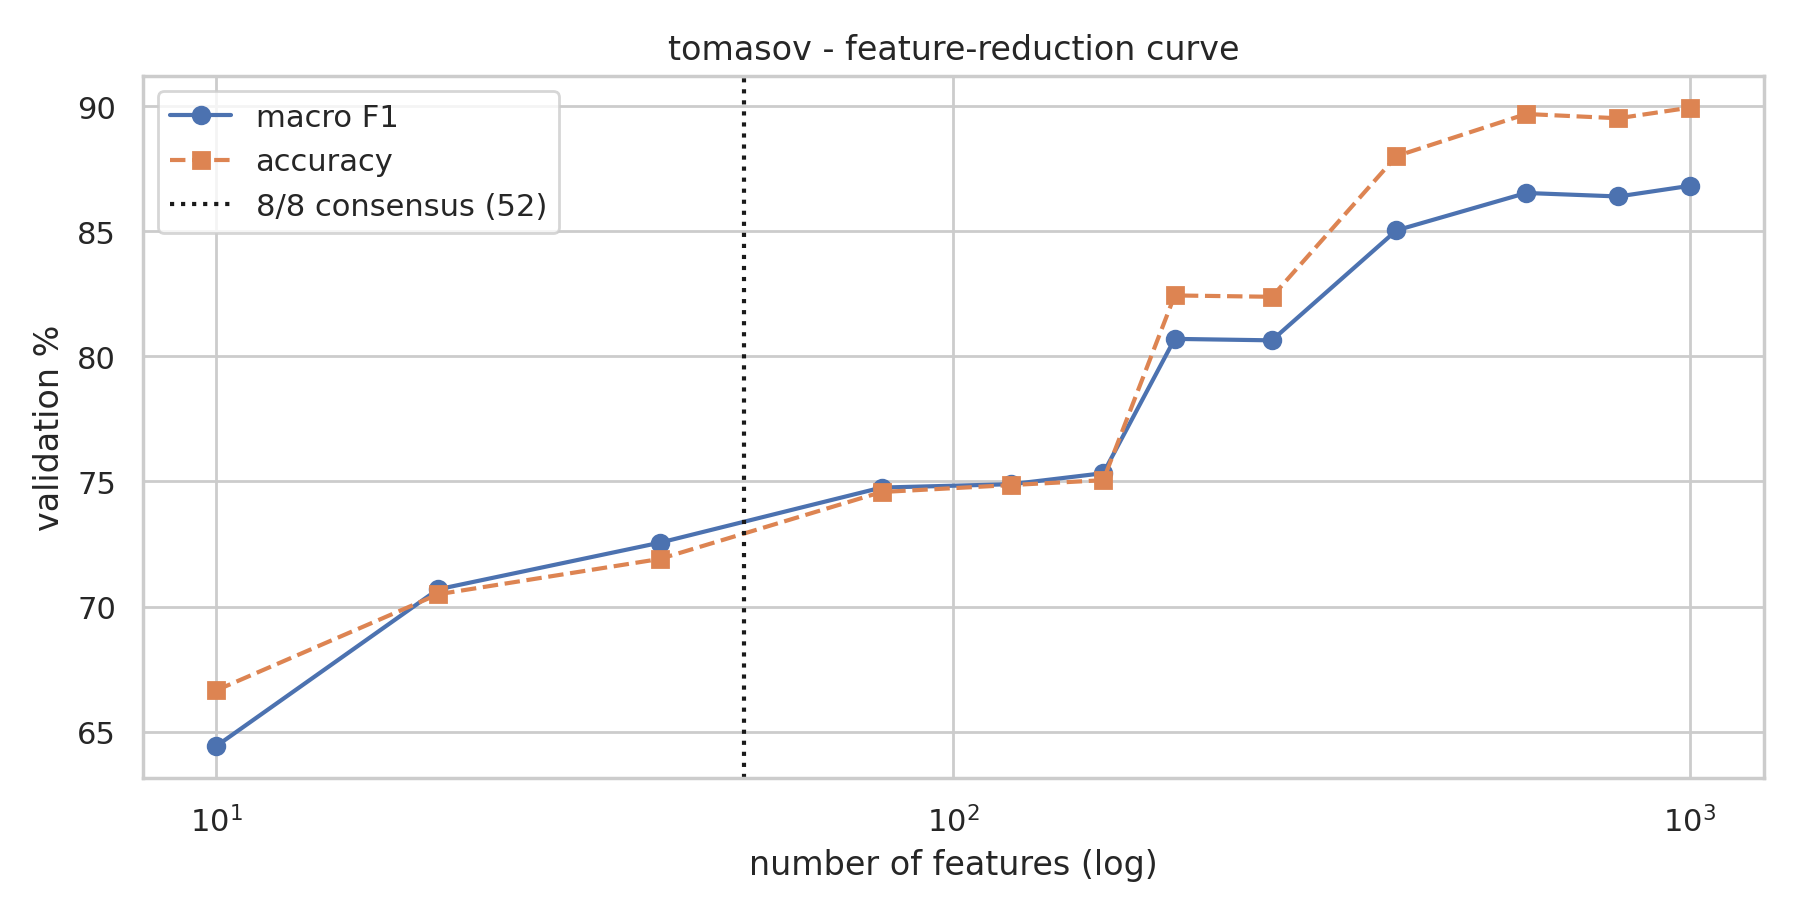
\includegraphics[width=0.48\textwidth,keepaspectratio]{Figures/fig17a_reduction_tomasov.png}
\hfill
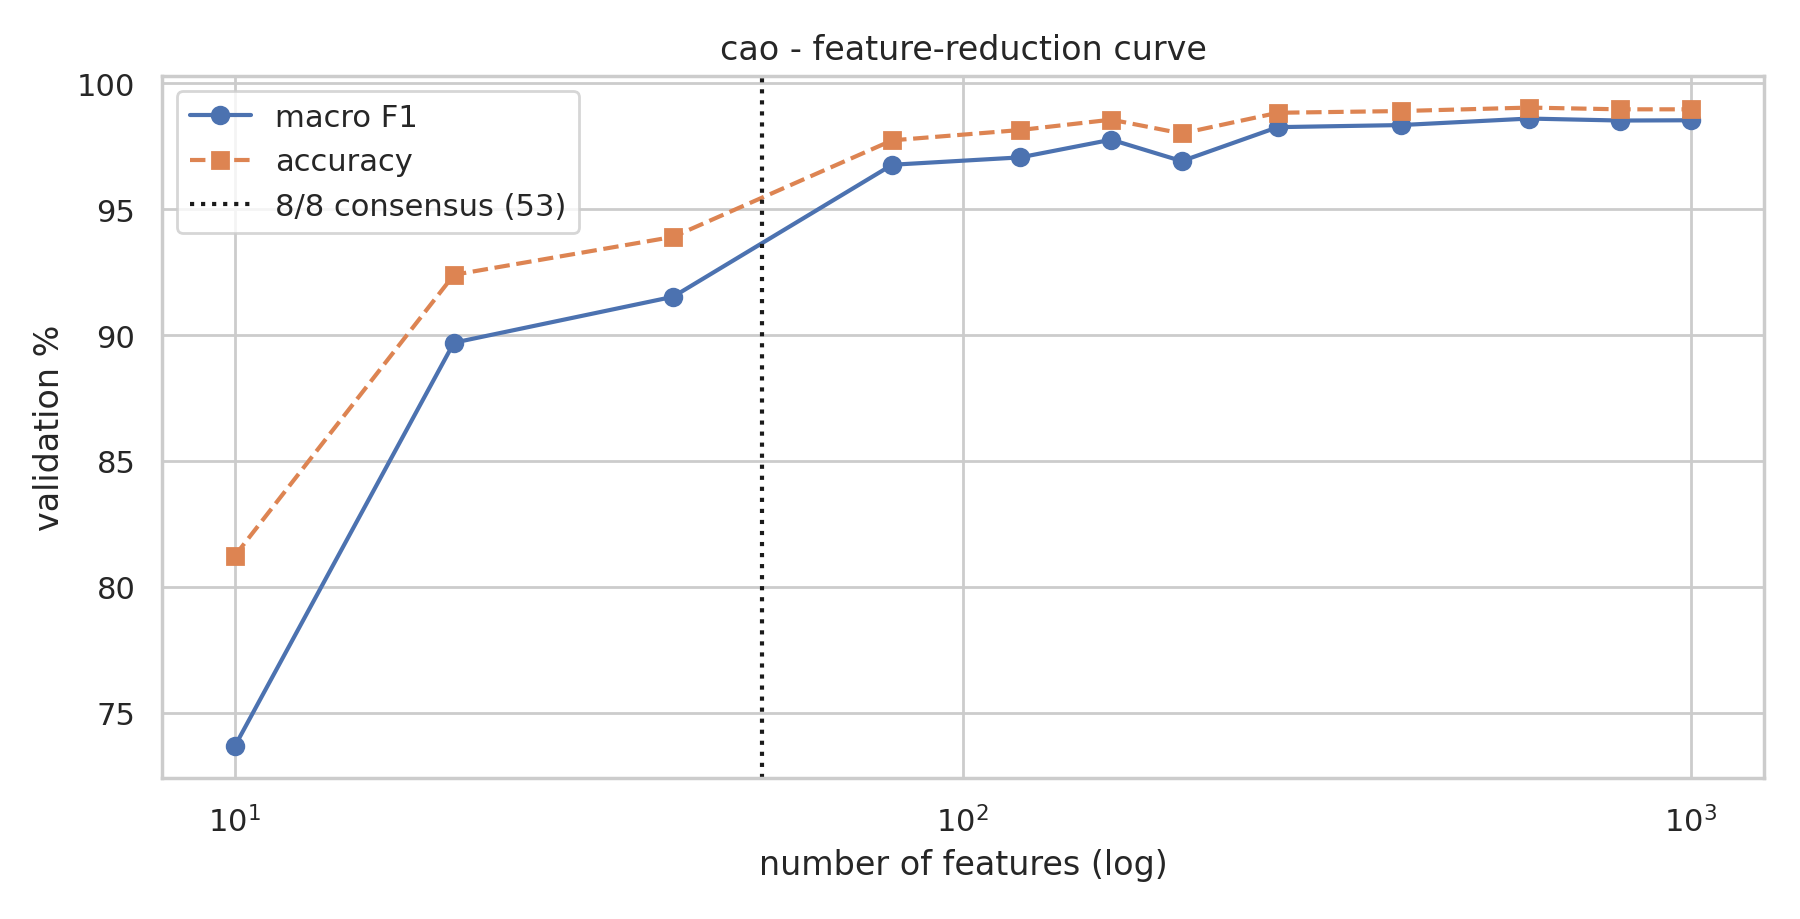
\includegraphics[width=0.48\textwidth,keepaspectratio]{Figures/fig17b_reduction_cao.png}
\caption{Validation performance against the number of retained features: Tomasov (left) and Cao (right).}
\label{fig:reduction}
\end{figure}

\subsection{Lightweight Effect of Feature Selection}
\label{sec:resSelectionLightweight}
\autoBookmark{subsec}{Lightweight Effect of Feature Selection}
\refss{sec:chap3LightweightSelection} identified four respects in which selection can reduce the cost of the pipeline. Table~\ref{tab:selection_footprint} reports each of them for the validation-selected LightGBM configuration on the full and the consensus feature sets. Model size follows the convention of \refss{sec:chap3Efficiency}: stored parameters at 32 bits each.

\begin{table}[!htbp]
	\centering
	\caption{Footprint of the selected LightGBM configuration with the full $1{,}002$-feature vector and with the unanimous consensus subset, on the Jetson AGX Orin. Training and inference run on the CPU. Each configuration uses its own validation-selected balancing strategy, so the training times include different resamplers.}
	\label{tab:selection_footprint}
	\footnotesize
	\setlength{\tabcolsep}{3.5pt}
	\begin{tabular}{@{}lrrrr@{}}
		\toprule
		& \multicolumn{2}{c}{\textbf{Tomasov}} & \multicolumn{2}{c}{\textbf{Cao}}\\
		\cmidrule(lr){2-3}\cmidrule(lr){4-5}
		\textbf{Measure} & \textbf{Full} & \textbf{Consensus} & \textbf{Full} & \textbf{Consensus}\\
		\midrule
		Descriptors per window      & 1{,}002 & 52 & 1{,}002 & 53\\
		Feature vector (bytes)      & 4{,}008 & 208 & 4{,}008 & 212\\
		Fused feature matrix (MB)   & 691.2 & 35.9 & 61.8 & 3.3\\
		Balancing strategy          & Borderline-SMOTE & SMOTE & Undersampling & Borderline-SMOTE\\
		Training time (s)           & 1{,}357.4 & \textbf{63.0} & 41.4 & \textbf{7.9}\\
		Inference (ms per window)   & 0.172 & \textbf{0.145} & \textbf{0.062} & 0.070\\
		Trees                       & 4{,}500 & 4{,}500 & 3{,}000 & 3{,}000\\
		Leaves                      & 288{,}000 & 288{,}000 & 71{,}526 & 121{,}130\\
		Stored parameters           & 855{,}000 & 855{,}000 & 208{,}578 & 357{,}390\\
		Model size, 32-bit (MB)            & 3.42 & 3.42 & \textbf{0.83} & 1.43\\
		Test macro-$F_1$                   & \textbf{81.98} & 73.59 & \textbf{98.90} & 93.08\\
		\bottomrule
	\end{tabular}
\end{table}

Selection substantially reduces the data and training costs of the pipeline. Each window is described by about $95\%$ fewer descriptors; a stored feature vector consequently decreases from $4{,}008$ to approximately 210 bytes and the Tomasov feature store from $691$\,MB to $36$\,MB. Training of the selected model is $21.5$ times faster on Tomasov ($1{,}357$ to $63$\,s) and $5.3$ times faster on Cao ($41$ to $8$\,s), which means that a consensus model can be retrained on the CPU of the embedded board in about one minute when a site or its mix of events changes.

Selection does not, however, make the fitted model smaller or faster to query, and the reason lies in the way in which the size of a boosted ensemble is determined. LightGBM grows one tree per class in each of 500 rounds, with at most 64 leaves per tree, irrespective of the number of input features. On Tomasov every one of the $4{,}500$ trees reaches 64 leaves with either feature set, so both models hold $855{,}000$ parameters ($3.42$\,MB), and inference changes only from $0.172$ to $0.145$\,ms. On Cao the consensus model is the larger of the two ($1.43$ against $0.83$\,MB), because its trees grow more leaves ($121{,}130$ against $71{,}526$), which is consistent with its having been trained on an oversampled rather than an undersampled training set. A smaller model would be obtained by reducing the number of rounds or leaves, not the number of features.

Nor does selection yet reduce the time required for feature extraction, the largest online cost. The extractor computes every domain in full, and the consensus subsets still draw on all four domains (Table~\ref{tab:consensus}), so the reported extraction time of \refs{sec:resEfficiency} applies to both configurations. Computing only the 52 or 53 retained descriptors is the step that would convert the saving in dimensionality into a saving in latency (\refss{sec:chap5FutureCost}).

Selection also incurs a one-time offline cost, $1{,}580$\,s on Tomasov and $1{,}260$\,s on Cao for all eight methods, most of which is attributable to Boruta, and a recurring cost in accuracy of $8.39$ and $5.81$ macro-$F_1$ points. The unanimous subset is therefore the lightweight operating point for storage, transmission, and retraining, the full vector is the operating point for accuracy, and the reduction curve of \reff{fig:reduction} provides the intermediate points between them.

\subsection{Fold-Wise Feature Selection}
\label{sec:resSelectionBias}
\autoBookmark{subsec}{Fold-Wise Feature Selection}
A recurrent criticism of feature-engineering pipelines is that fitting selection once on the training split and then cross-validating on that split inflates the estimate. The controlled comparison of \refss{sec:chap3ConfoundDesign} measured this effect directly by evaluating the identical model on the same grouped folds, once with selection fitted before cross-validation and once with selection refitted in every fold. At this data scale the effect is negligible: the optimism is $+0.02$ points on Tomasov and $-0.19$ on Cao, both within the confidence intervals. With $148{,}229$ and $12{,}155$ training rows, the eight-method consensus is sufficiently stable that its position relative to the fold boundary does not measurably change the estimate. Fold-wise selection remains the correct practice, particularly for smaller datasets, but in this setting the optimism of earlier results is attributable to partition leakage rather than to the placement of feature selection.

\section{Training Set Balancing Strategies}
\label{sec:resBalancing}
\autoBookmark{sec}{Training Set Balancing Strategies}
Each of the six balancing strategies is applied to the training set alone, after feature selection and immediately before modelling, which leaves the validation and test distributions unaltered. \reff{fig:heatmaps} shows the validation macro-$F_1$ for every (classifier, strategy) pair, and two patterns are evident. The gradient-boosting family occupies the top three rows on both datasets by a clear margin, and within any row the six columns differ by a fraction of that margin. Averaged over the seven classifiers, the range of test macro-$F_1$ across strategies is $1.94$ points on Tomasov and $0.44$ on Cao, the former well within the $\pm 4.42$-point partition standard deviation reported in \refs{sec:resStats}. Validation selects Borderline-SMOTE for Tomasov and random undersampling for Cao, but the second- and third-ranked strategies are lower by only a few tenths of a point.

\begin{figure}[!htbp]
\centering
\begin{subfigure}[b]{0.49\textwidth}
	\centering
	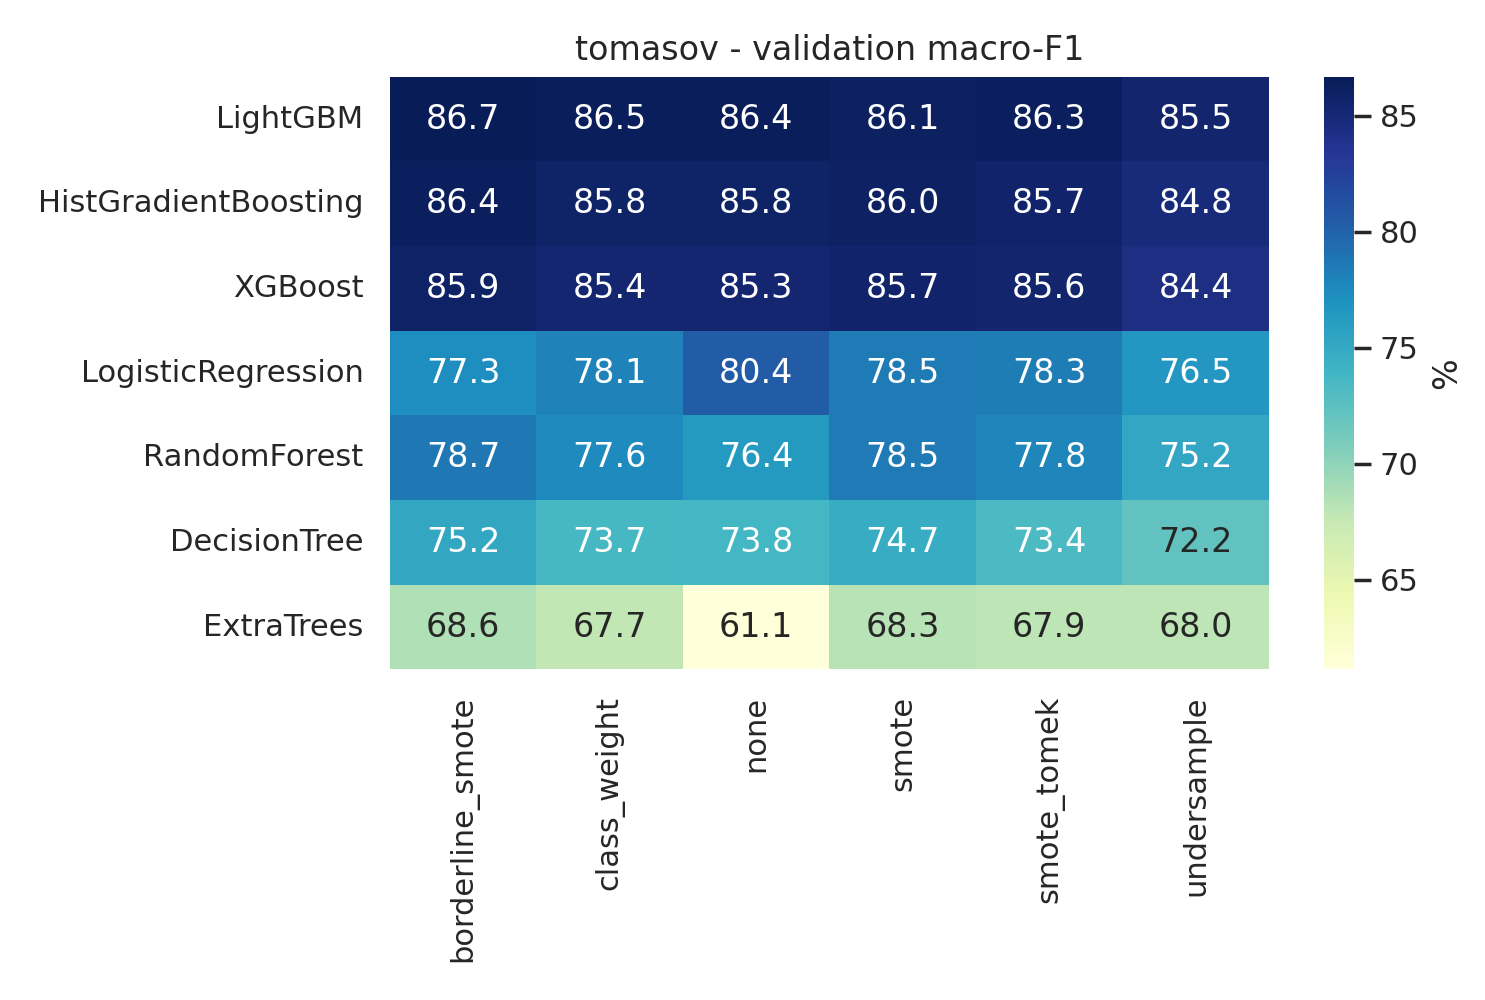
\includegraphics[width=\textwidth,keepaspectratio]{Figures/fig29a_heatmap_tomasov.png}
	\caption{Tomasov 2025}
\end{subfigure}\hfill
\begin{subfigure}[b]{0.49\textwidth}
	\centering
	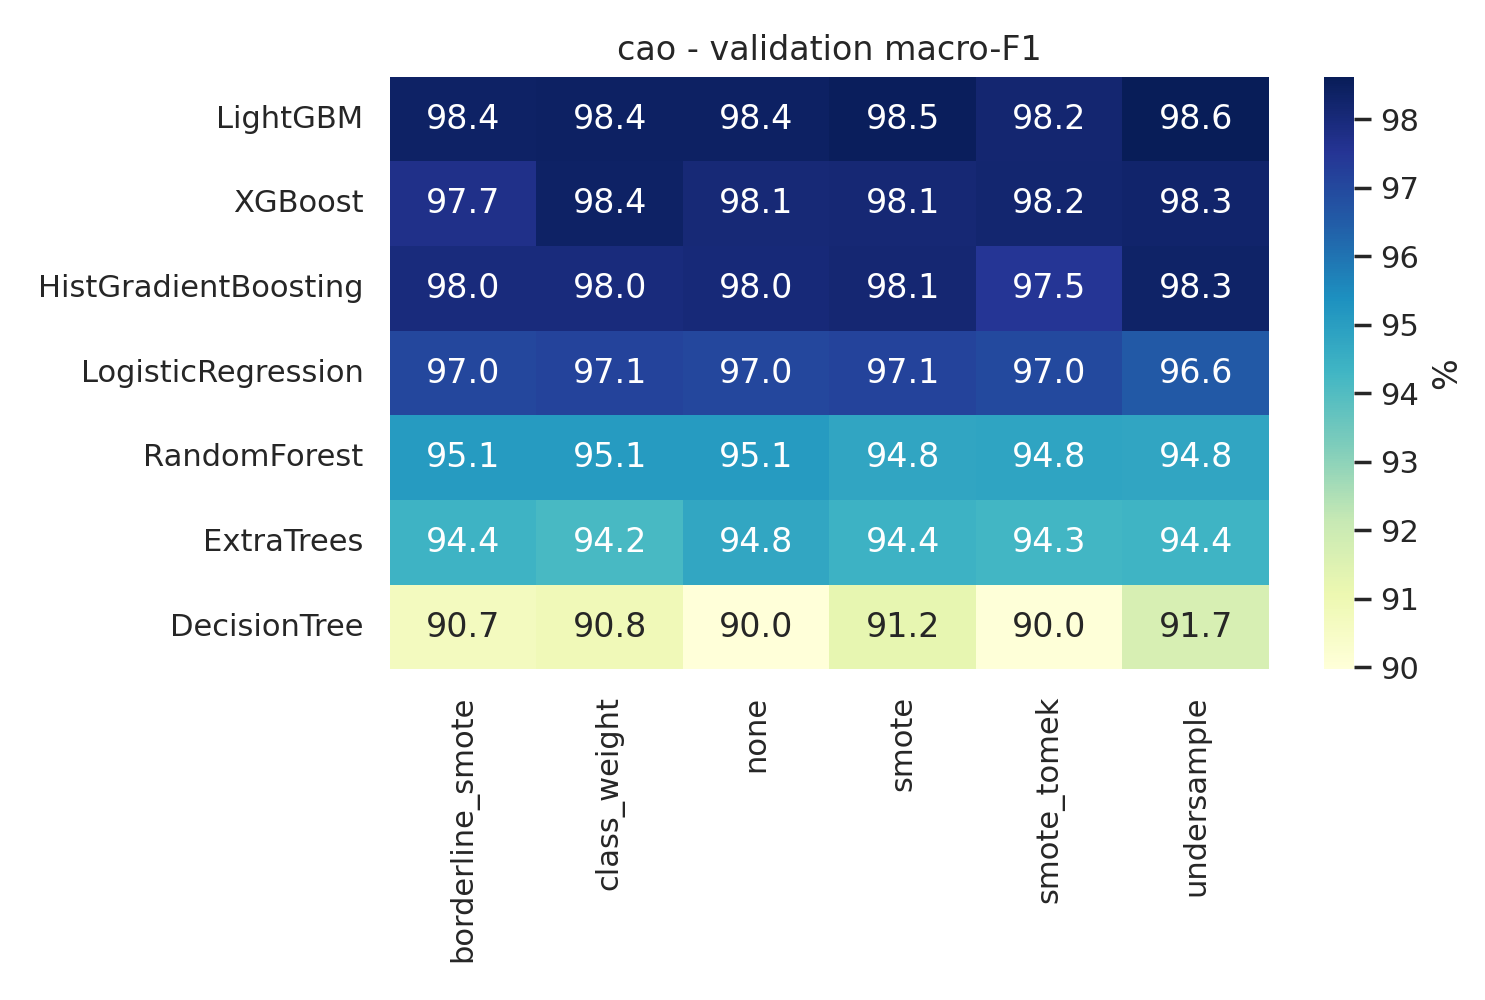
\includegraphics[width=\textwidth,keepaspectratio]{Figures/fig29b_heatmap_cao.png}
	\caption{Cao 2023}
\end{subfigure}
\caption{Validation macro-$F_1$ (\%) for every classifier and balancing strategy on the full $1{,}002$-feature representation. Rows are ordered by mean performance.}
\label{fig:heatmaps}
\end{figure}

These results do not support a consistent advantage for cost-sensitive class weighting. When the strategies are compared over independent held-out acquisitions (\refs{sec:resStats}), two pairs can be distinguished on Tomasov, by a margin that reflects recall on single-class recordings rather than general classification quality, and no pair can be distinguished on Cao. Computational cost is therefore the more useful criterion. Class weighting and the no-balancing baseline both avoid the synthetic-sample generation and training-set inflation of the SMOTE family, which on Tomasov approximately doubles the fitting time ($1{,}756$\,s for Borderline-SMOTE against $798$\,s for class weighting) without a reliable gain. This result answers the class-balancing part of \textbf{RQ2}; together with \refs{sec:resDomains} and \refs{sec:resSelection} it establishes the representation and training components, and \refs{sec:resFinal} adds the choice of classifier.

\section{Modelling}
\label{sec:resFinal}
\autoBookmark{sec}{Modelling}
The modelling stage of \reff{fig:methodology_framework} trains seven classifiers on every combination of feature set and balancing strategy and uses the validation set to choose among them. Each classifier is represented by the balancing strategy that maximised its own validation macro-$F_1$, which yields one configuration per classifier chosen by the same rule, and the configuration with the highest validation macro-$F_1$ across classifiers is the selected model. \refss{sec:resAllModels} compares the seven classifiers on effectiveness and cost, and \refss{sec:resSelected} reports the selected configuration and its generalisation gap. \refs{sec:resPerformance} then examines the per-class behaviour of all seven.

\subsection{Classifier Comparison}
\label{sec:resAllModels}
\autoBookmark{subsec}{Classifier Comparison}
Table~\ref{tab:all_models} reports the seven classifiers on both datasets, on each of which they form the same three tiers. The gradient-boosting family (LightGBM, XGBoost, and histogram-based gradient boosting) occupies the top three positions, and its members lie within $0.62$ macro-$F_1$ points of one another on Tomasov and $0.84$ on Cao. Logistic regression forms a second tier, $3.38$ points behind LightGBM on Tomasov but only $1.06$ behind on Cao. The bagged ensembles and the single decision tree form the third tier. The best and worst classifiers differ by $14.32$ points on Tomasov and $7.34$ on Cao; the choice of learner is thus about twice as consequential on the more difficult dataset.

\begin{table}[!htbp]
	\centering
	\caption{All seven classifiers on the full $1{,}002$-feature representation, each at the balancing strategy that maximised its own validation macro-$F_1$, ordered by validation macro-$F_1$. Test metrics in \%. The consensus column gives test macro-$F_1$ on the unanimous subset, again at each classifier's own validation-selected strategy. Times are from the benchmark run on the Jetson AGX Orin and can differ slightly from the final-model timings of Table~\ref{tab:main_results}.}
	\label{tab:all_models}
	\footnotesize
	\setlength{\tabcolsep}{3pt}
	\resizebox{\textwidth}{!}{%
	\begin{tabular}{@{}llrrrrrrrr@{}}
		\toprule
		\textbf{Classifier} & \textbf{Balancing} & \textbf{Val.\ $F_1$} & \textbf{Acc.} & \textbf{Bal.\ acc.} & \textbf{Macro-$F_1$} & \textbf{AUC} & \textbf{Train (s)} & \textbf{Infer.\ (ms)} & \textbf{Consensus $F_1$}\\
		\midrule
		\multicolumn{10}{@{}l}{\textit{Tomasov \etal\ 2025 (9 classes)}}\\[2pt]
		LightGBM             & Borderline-SMOTE & \textbf{86.69} & \textbf{90.71} & \textbf{81.97} & 81.98 & 97.46 & 1{,}393.1 & 0.183  & 73.59\\
		HistGradientBoosting & Borderline-SMOTE & 86.35 & 90.50 & 81.96 & \textbf{82.12} & \textbf{97.52} & 1{,}880.7 & 0.223  & 73.19\\
		XGBoost              & Borderline-SMOTE & 85.93 & 90.37 & 81.60 & 81.50 & 96.45 & 4{,}285.6 & 0.046  & \textbf{73.68}\\
		LogisticRegression   & None             & 80.41 & 84.38 & 77.68 & 78.59 & 96.95 & 1{,}070.6 & 0.011  & 67.76\\
		RandomForest         & Borderline-SMOTE & 78.67 & 82.72 & 75.63 & 75.63 & 94.66 & 914.7     & 0.030  & 72.09\\
		DecisionTree         & Borderline-SMOTE & 75.16 & 79.83 & 70.96 & 71.69 & 87.49 & 1{,}039.7 & 0.001  & 64.27\\
		ExtraTrees           & Borderline-SMOTE & 68.60 & 72.38 & 68.72 & 67.80 & 93.31 & 398.0     & 0.034  & 66.92\\
		\midrule
		\multicolumn{10}{@{}l}{\textit{Cao \etal\ 2023 (6 classes)}}\\[2pt]
		LightGBM             & Undersampling    & \textbf{98.62} & \textbf{99.06} & \textbf{98.98} & \textbf{98.90} & \textbf{99.99} & 40.2      & 0.067  & \textbf{93.08}\\
		XGBoost              & Class weighting  & 98.36 & 98.61 & 98.54 & 98.38 & 99.98 & 173.4     & 0.012  & 92.53\\
		HistGradientBoosting & Undersampling    & 98.32 & 98.45 & 98.13 & 98.06 & 99.96 & 44.5      & 0.019  & 92.17\\
		LogisticRegression   & Class weighting  & 97.14 & 98.23 & 98.16 & 97.84 & 99.96 & 8.6       & 0.025  & 88.09\\
		RandomForest         & None             & 95.08 & 97.50 & 97.58 & 97.21 & 99.90 & 12.6      & 0.074  & 91.50\\
		ExtraTrees           & None             & 94.76 & 97.00 & 96.95 & 96.51 & 99.89 & 3.9       & 0.079  & 91.20\\
		DecisionTree         & Undersampling    & 91.68 & 92.73 & 92.30 & 91.56 & 94.97 & 16.8      & 0.001  & 84.74\\
		\bottomrule
	\end{tabular}}
\end{table}

The validation rule selects LightGBM in all four combinations of dataset and feature set, but the test ordering within the boosting tier does not always agree with it. On the full Tomasov representation, histogram-based gradient boosting reaches a test macro-$F_1$ of $82.12$ against $81.98$ for LightGBM, and on the Tomasov consensus subset XGBoost reaches $73.68$ against $73.59$. These reversals of $0.14$ and $0.09$ points are a small fraction of the $\pm 4.42$-point partition standard deviation on Tomasov (\refs{sec:resStats}), so the three boosted learners cannot be distinguished on these data. The defensible conclusion for the development of the pipeline (\textbf{RQ2}) is therefore that it performs best with a gradient-boosting learner, with LightGBM as the member selected by the validation rule rather than a member shown to outperform the other two.

Logistic regression performs better than its linear form might suggest. On Cao it is only $1.06$ points below LightGBM while training in $8.6$\,s, which indicates that the fused descriptors render the six Cao classes close to linearly separable. It is, however, the learner that depends most strongly on the full representation: the consensus subsets reduce its score by $10.83$ points on Tomasov and $9.75$ on Cao, compared with $8.39$ and $5.81$ for LightGBM, which is consistent with a linear model that combines many weakly informative features that the unanimity rule discards. The bagged ensembles exhibit the opposite pattern. On the full Tomasov representation, extremely randomised trees fall below the single decision tree in macro-$F_1$ ($67.80$ against $71.69$) despite a higher one-vs-rest AUC ($93.31$ against $87.49$), which indicates that their probability rankings separate the classes better than their decisions do. On the 52-feature consensus subset the same model loses only $0.88$ points and random forest only $3.54$, against $8.39$ for LightGBM. Both observations indicate dilution by uninformative columns. The bagged ensembles consider only 31 randomly drawn features at each split, the square root of $1{,}002$, so on the full representation many candidate splits involve no informative feature, whereas the boosted learners search at least $80\%$ of the features at every split and are largely unaffected. The weaker learners are also more sensitive to the balancing strategy: across the six strategies, test macro-$F_1$ varies by $6.66$ points for extremely randomised trees on Tomasov but by only $0.63$ for LightGBM.

Within the top tier, computational cost distinguishes the classifiers more clearly than effectiveness does. On Tomasov, XGBoost requires $4{,}286$\,s to train compared with $1{,}393$\,s for LightGBM but predicts a window in $0.046$\,ms rather than $0.183$\,ms, and histogram-based gradient boosting is the slowest of the three at prediction. Every classifier predicts a window in well under a millisecond on the CPU of the Jetson AGX Orin, between two and five orders of magnitude below the window-arrival intervals of $102.4$\,ms (Tomasov) and $204.8$\,ms (Cao). Inference cost therefore does not discriminate between the learners in deployment; training cost does, and, as \refs{sec:resEfficiency} shows, so does feature extraction.

\subsection{Selection on the Validation Set}
\label{sec:resSelected}
\autoBookmark{subsec}{Selection on the Validation Set}
Table~\ref{tab:main_results} reports the configuration selected on validation for each dataset and feature set. LightGBM is selected in all four cases, subject to the qualification stated above, and this selected configuration is the one compared with the published and recent baselines in the Discussion (\refs{sec:resDiscussion}). With the full feature set it reaches $90.71\%$ accuracy and $81.98$ macro-$F_1$ on the nine-class Tomasov dataset and $99.06\%$ accuracy and $98.90$ macro-$F_1$ on the six-class Cao dataset, with inference below $0.2$\,ms per window. The pipeline designed on the primary dataset is thus applied unchanged to the evaluation dataset, with the same settings and without per-dataset tuning, which completes the development required by \textbf{RQ2}.

\begin{table}[!htbp]
	\centering
	\caption{Final results under the leakage-controlled protocol, measuring segment-level generalisation within represented recordings. Model and balancing strategy selected on validation; test metrics reported once.}
	\label{tab:main_results}
	\footnotesize
	\setlength{\tabcolsep}{3.5pt}
	\resizebox{\textwidth}{!}{%
\begin{tabular}{@{}lllrrrrrr@{}}
		\toprule
		\textbf{Dataset} & \textbf{Feature set} & \textbf{Balancing} & \textbf{Feat.} & \textbf{Acc. (\%)} & \textbf{Bal. acc.} & \textbf{Macro-$F_1$} & \textbf{CV $F_1$} & \textbf{Infer. (ms)}\\
		\midrule
		Tomasov (9 cls) & Multi-domain  & Borderline-SMOTE & 1{,}002 & \textbf{90.71} & \textbf{81.97} & \textbf{81.98} & 78.60 & 0.172\\
		Tomasov (9 cls) & Consensus 8/8 & SMOTE            & 52      & 77.29          & 72.88          & 73.59          & 66.25 & 0.145\\
		Cao (6 cls)     & Multi-domain  & Undersampling    & 1{,}002 & \textbf{99.06} & \textbf{98.98} & \textbf{98.90} & 98.51 & 0.062\\
		Cao (6 cls)     & Consensus 8/8 & Borderline-SMOTE & 53      & 94.40          & 93.36          & 93.08          & 93.93 & 0.070\\
		\bottomrule
	\end{tabular}}
\end{table}

For the full feature set, the held-out test macro-$F_1$ exceeds the cross-validated estimate by $3.38$ points on Tomasov and $0.38$ on Cao, which indicates that the $1{,}002$-dimensional representation does not overfit substantially; the larger Tomasov gap is consistent with the greater heterogeneity of its recordings. These figures measure generalisation to unseen segments of recordings that are represented in training. \refs{sec:resGeneralisation} reports the cross-recording measurement, which is available for the four Tomasov classes recorded more than once and yields $63.85\%$ accuracy. The figures also retain the numerical residue in the normalisation that a subsequent audit of the feature code identified; \refss{sec:chap5LimResidue} reports its magnitude, which is substantial on Tomasov and small on Cao.

\section{Performance Evaluation}
\label{sec:resPerformance}
\autoBookmark{sec}{Performance Evaluation}
The performance evaluation stage of \reff{fig:methodology_framework} scores every model with accuracy, precision, recall, and $F_1$ on the same test windows. \refs{sec:resFinal} compared the seven classifiers on aggregate metrics, and the Discussion (\refs{sec:resDiscussion}) compares them with the models of the baseline branch. This section examines per-class behaviour, in which the differences between learners and the limits of the representation become apparent. \refss{sec:resPerClass} reports the per-class $F_1$ of all seven classifiers, \refss{sec:resOpenclose} examines the class that no feature-based classifier recovers, and \refss{sec:resErrors} examines the remaining dominant error mode.

\subsection{Per-Class Performance}
\label{sec:resPerClass}
\autoBookmark{subsec}{Per-Class Performance}
Table~\ref{tab:per_class} gives the test $F_1$ of every class for all seven classifiers, and \reff{fig:confusion_tomasov} and \reff{fig:confusion_cao} show the confusion matrices of the selected LightGBM configuration. The per-class values were obtained by retraining each classifier at its validation-selected strategy on the frozen partition. The retrained models match the benchmark of Table~\ref{tab:all_models} to the second decimal place for every classifier except two, and in neither case is the difference sufficient to alter a comparison: logistic regression on Tomasov, whose L-BFGS solver stops at its iteration limit before formal convergence, differs by $0.16$ macro-$F_1$ points, and XGBoost differs by $0.14$ on Tomasov and by less than $0.01$ on Cao.

\begin{table}[!htbp]
	\centering
	\caption{Per-class test $F_1$ of all seven classifiers on the full $1{,}002$-feature representation, each at its validation-selected balancing strategy. The best value in each row is in bold; $n$ is the test support. LGBM: LightGBM; XGB: XGBoost; HGB: histogram-based gradient boosting; LR: logistic regression; RF: random forest; ET: extremely randomised trees; DT: decision tree.}
	\label{tab:per_class}
	\footnotesize
	\setlength{\tabcolsep}{4pt}
	\begin{tabular}{@{}lrrrrrrrr@{}}
		\toprule
		\textbf{Class} & \textbf{$n$} & \textbf{LGBM} & \textbf{XGB} & \textbf{HGB} & \textbf{LR} & \textbf{RF} & \textbf{ET} & \textbf{DT}\\
		\midrule
		\multicolumn{9}{@{}l}{\textit{Tomasov \etal\ 2025}}\\[2pt]
		Car           &   1{,}772 & 0.845 & 0.831 & \textbf{0.846} & 0.728 & 0.729 & 0.581 & 0.751\\
		Construction  &   2{,}232 & \textbf{0.996} & 0.994 & 0.995 & 0.971 & 0.963 & 0.929 & 0.969\\
		Fence         &   1{,}983 & \textbf{0.893} & 0.889 & 0.889 & 0.769 & 0.731 & 0.505 & 0.804\\
		Longboard     &       581 & 0.912 & 0.913 & 0.906 & 0.910 & \textbf{0.933} & 0.887 & 0.736\\
		Manipulation  &       867 & \textbf{0.993} & 0.986 & \textbf{0.993} & 0.967 & 0.935 & 0.881 & 0.817\\
		Openclose     &       198 & 0.044 & 0.018 & 0.074 & \textbf{0.189} & 0.000 & 0.035 & 0.042\\
		Regular       &   1{,}111 & 0.847 & \textbf{0.849} & 0.844 & 0.738 & 0.705 & 0.566 & 0.757\\
		Running       &       929 & 0.946 & \textbf{0.948} & 0.944 & 0.945 & 0.947 & 0.933 & 0.787\\
		Walk          &   1{,}661 & \textbf{0.903} & 0.897 & 0.900 & 0.871 & 0.863 & 0.784 & 0.790\\
		\midrule
		\multicolumn{9}{@{}l}{\textit{Cao \etal\ 2023}}\\[2pt]
		Background    &       227 & \textbf{0.996} & \textbf{0.996} & \textbf{0.996} & 0.989 & 0.987 & 0.983 & 0.965\\
		Digging       &       370 & \textbf{0.988} & 0.987 & \textbf{0.988} & 0.985 & 0.967 & 0.973 & 0.911\\
		Knocking      &       622 & \textbf{0.998} & 0.995 & 0.995 & 0.990 & 0.986 & 0.982 & 0.968\\
		Shaking       &       134 & \textbf{0.993} & 0.978 & 0.978 & 0.960 & 0.968 & 0.950 & 0.901\\
		Walking       &       232 & \textbf{0.976} & 0.963 & 0.955 & 0.969 & 0.950 & 0.938 & 0.847\\
		Watering      &       218 & \textbf{0.984} & \textbf{0.984} & 0.972 & 0.977 & 0.975 & 0.965 & 0.901\\
		\bottomrule
	\end{tabular}
\end{table}

The Tomasov dataset differentiates the learners far more than the Cao dataset does, and the per-class pattern shows where the differences arise. The boosted learners lead on seven of the nine classes, and that lead is shared among all three: LightGBM is best on four classes, XGBoost on two, and histogram-based gradient boosting on one, which is consistent with the conclusion of \refss{sec:resAllModels} that the three cannot be distinguished. Random forest is best on \emph{longboard} ($0.933$), and logistic regression is best on \emph{openclose}, although only at $0.189$. The learners differ most on \emph{fence}, \emph{regular}, and \emph{car}, with spreads of $0.388$, $0.282$, and $0.265$, and these are the three classes involved in the dominant confusions examined below. Three of the five single-recording classes, \emph{construction}, \emph{manipulation}, and \emph{running}, reach at least $0.88$ for every learner except the single decision tree; as \refs{sec:resConfound} shows, high scores on such classes cannot be separated from recognition of the recording itself. Table~\ref{tab:error_modes} traces the two dominant error modes across all seven learners, and both occur in every one of them.

On Cao the ranking of the classes is almost identical for every learner. The three boosted learners exceed an $F_1$ of $0.95$ on every class, and \emph{walking} is the weakest class for six of the seven classifiers, ranging from $0.847$ for the decision tree to $0.976$ for LightGBM. Its errors are assigned mainly to \emph{digging}, which receives between $1.3\%$ (LightGBM) and $6.9\%$ (decision tree) of the walking windows. Logistic regression is the exception: it misclassifies only $0.4\%$ of the walking windows in this way, and its weakest class is \emph{shaking} at $0.960$. The spread between the best and worst learner is smallest for \emph{background} and \emph{knocking} ($0.030$) and largest for \emph{walking} ($0.129$); the learners thus differ most on the class whose signature overlaps with those of other classes and least on the classes with distinctive signatures.

\begin{figure}[!htbp]
\centering
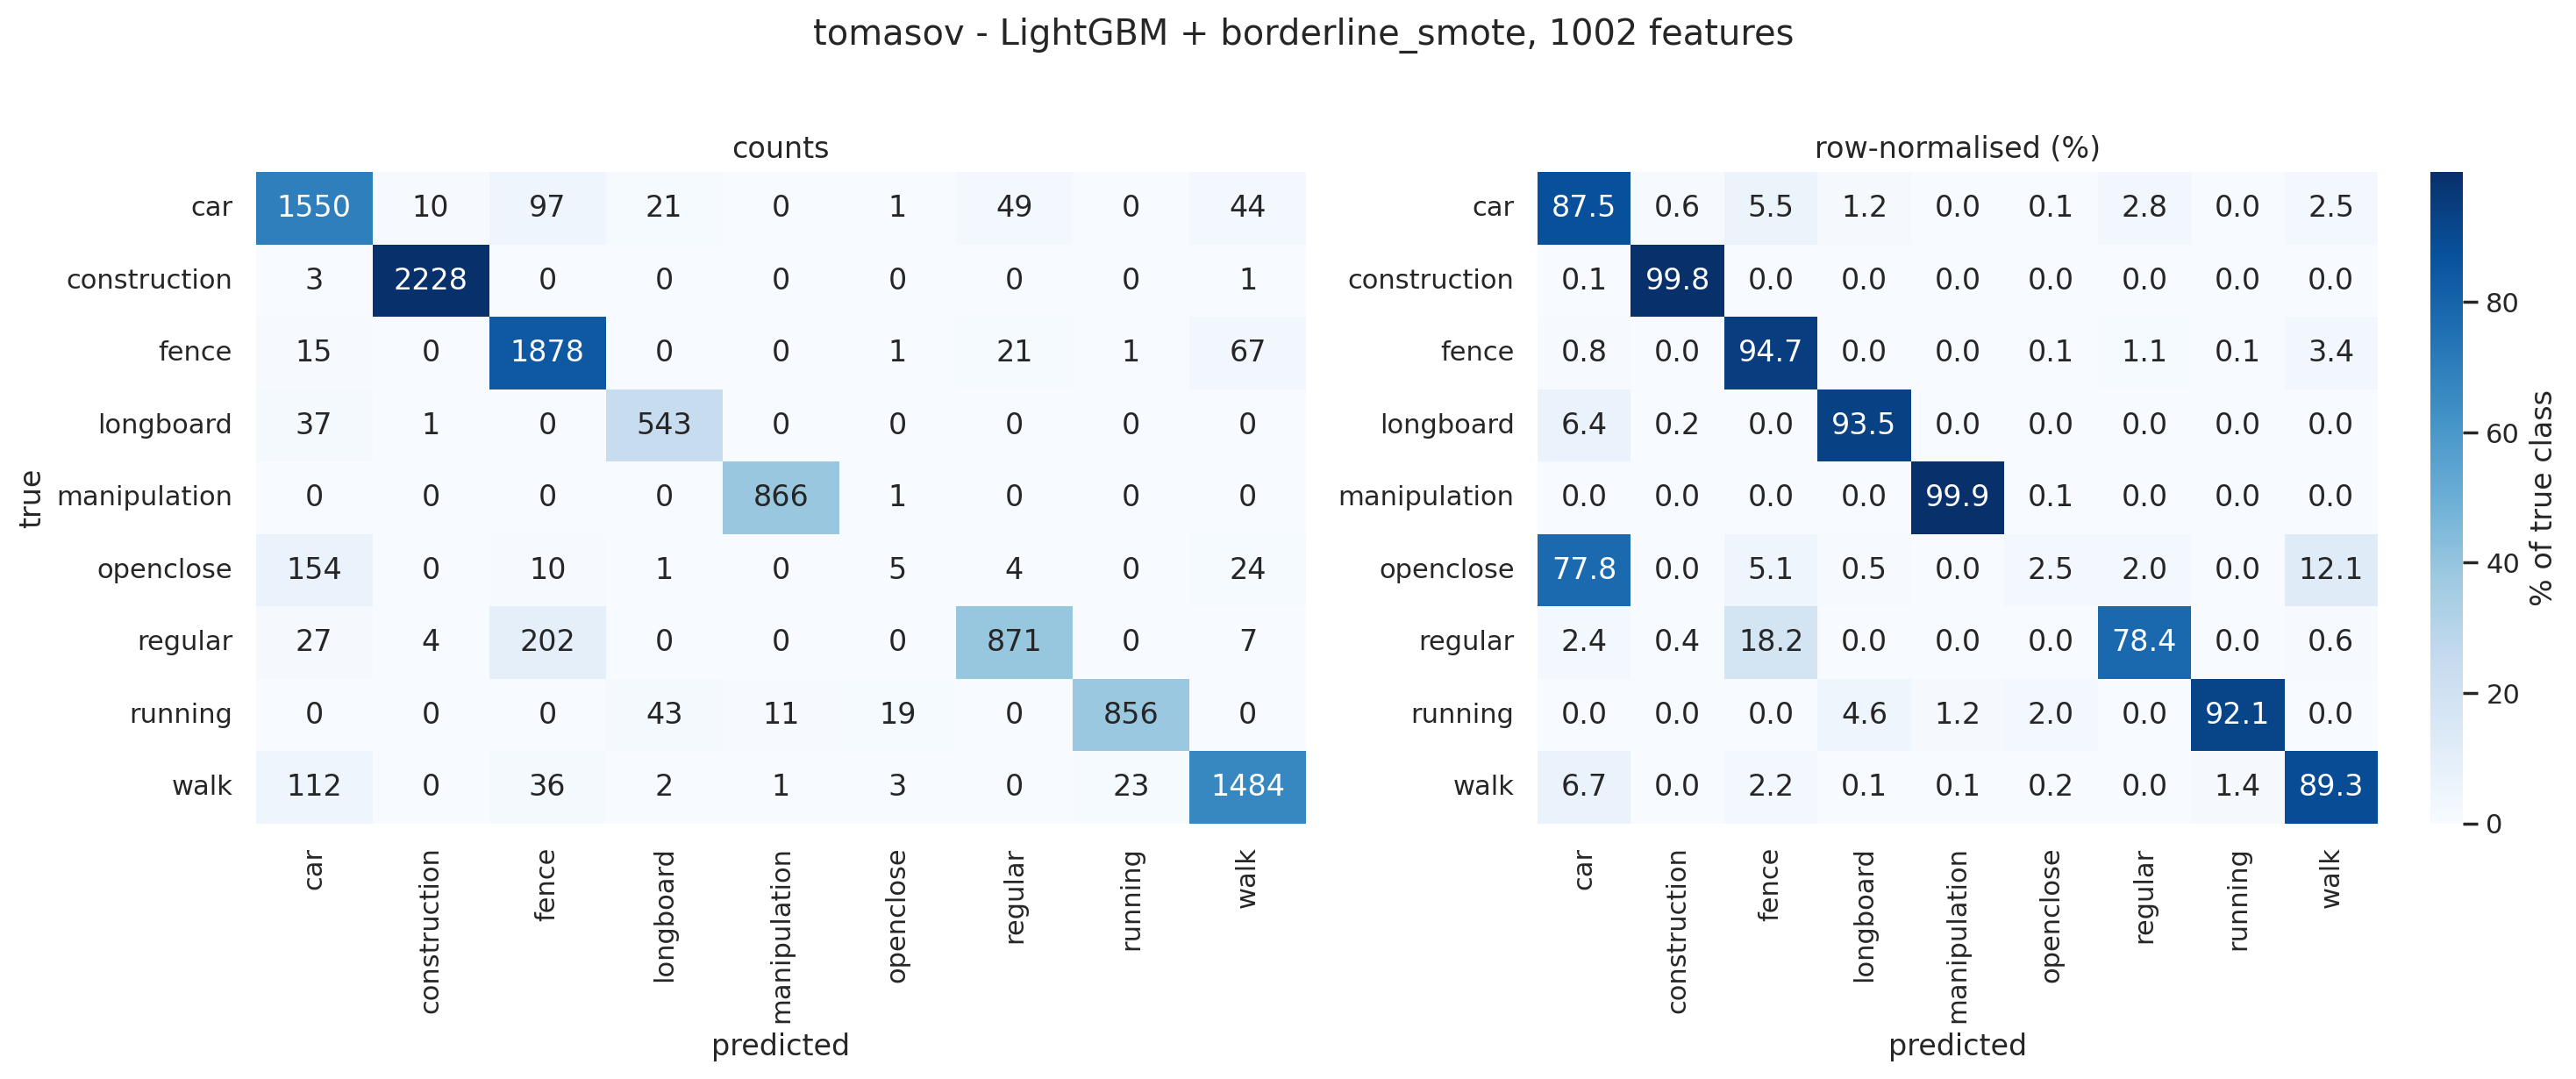
\includegraphics[width=0.9\textwidth,keepaspectratio]{Figures/fig19_confusion_tomasov.png}
\caption{Row-normalised confusion matrix of the selected LightGBM configuration, Tomasov 2025, multi-domain feature set.}
\label{fig:confusion_tomasov}
\end{figure}

\begin{figure}[!htbp]
\centering
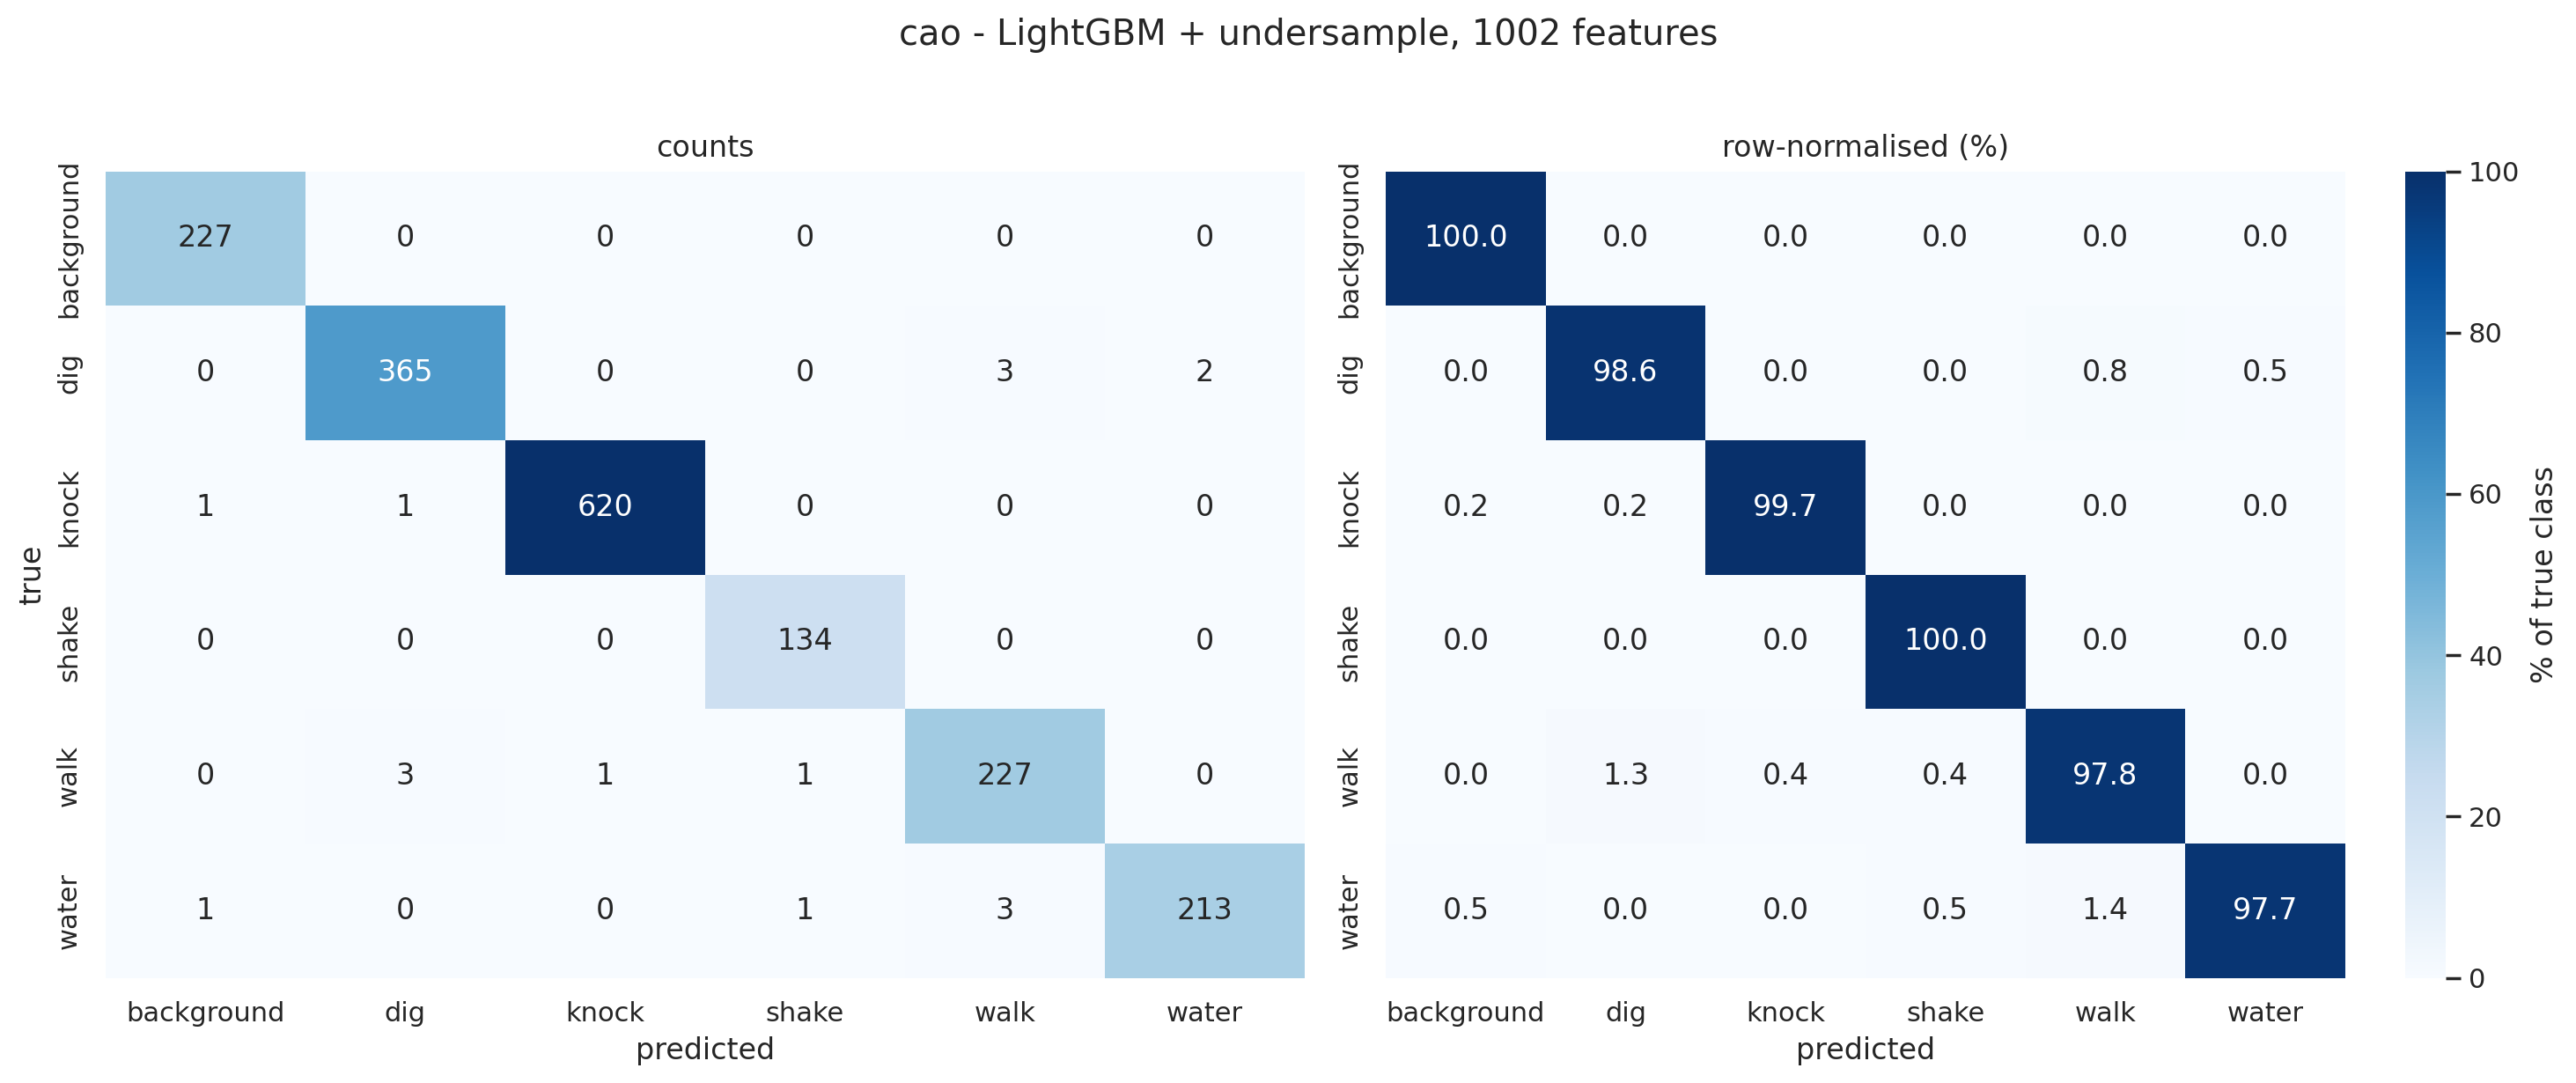
\includegraphics[width=0.9\textwidth,keepaspectratio]{Figures/fig20_confusion_cao.png}
\caption{Row-normalised confusion matrix of the selected LightGBM configuration, Cao 2023, multi-domain feature set.}
\label{fig:confusion_cao}
\end{figure}

\subsection{Performance on the \emph{Openclose} Class}
\label{sec:resOpenclose}
\autoBookmark{subsec}{Performance on the Openclose Class}
The most consequential single result is that none of the seven classifiers recognises \emph{openclose} (Table~\ref{tab:error_modes}). Its $F_1$ ranges from $0.000$ for random forest to $0.189$ for logistic regression; for the selected LightGBM it is $0.044$ with $2.5\%$ recall, with $77.8\%$ of its test windows classified as \emph{car} and a further $12.1\%$ as \emph{walk}. Every learner assigns the largest share of the class to \emph{car}, between $42.9\%$ (extremely randomised trees) and $91.4\%$ (random forest) of its windows, and all seven assign the next largest share to \emph{walk}. Under the previously published protocol the same class attained an $F_1$ of $0.72$ with $70\%$ recall.

\begin{table}[!htbp]
	\centering
	\caption{The two dominant Tomasov error modes across all seven classifiers. P, R, and $F_1$ refer to \emph{openclose}; the arrows give the percentage of a true class's test windows assigned to the named class; the last column is the recall of \emph{regular}.}
	\label{tab:error_modes}
	\footnotesize
	\setlength{\tabcolsep}{4pt}
	\begin{tabular}{@{}lrrrrrrr@{}}
		\toprule
		& \multicolumn{5}{c}{\textbf{\emph{Openclose}} ($n = 198$)} & \multicolumn{2}{c}{\textbf{\emph{Regular}} ($n = 1{,}111$)}\\
		\cmidrule(lr){2-6}\cmidrule(lr){7-8}
		\textbf{Classifier} & \textbf{P} & \textbf{R} & \textbf{$F_1$} & \textbf{$\rightarrow$ car (\%)} & \textbf{$\rightarrow$ walk (\%)} & \textbf{$\rightarrow$ fence (\%)} & \textbf{R}\\
		\midrule
		LightGBM             & 0.167 & 0.025 & 0.044 & 77.8 & 12.1 & 18.2 & 0.784\\
		XGBoost              & 0.077 & 0.010 & 0.018 & 83.3 & 9.1 & 16.9 & 0.793\\
		HistGradientBoosting & 0.205 & 0.045 & 0.074 & 76.3 & 9.1 & 18.4 & 0.779\\
		LogisticRegression   & 0.379 & 0.126 & 0.189 & 54.0 & 21.7 & 32.7 & 0.650\\
		RandomForest         & 0.000 & 0.000 & 0.000 & 91.4 & 5.1 & 21.9 & 0.767\\
		ExtraTrees           & 0.043 & 0.030 & 0.035 & 42.9 & 30.8 & 12.7 & 0.857\\
		DecisionTree         & 0.032 & 0.061 & 0.042 & 79.8 & 8.6 & 19.3 & 0.732\\
		\bottomrule
	\end{tabular}
\end{table}

The earlier result was made possible by contamination. \emph{Openclose} is the smallest class ($6{,}792$ windows, $1.54\%$ of the annotated set) and originates from a single recording. A random split places neighbouring windows from that recording in the training set and allows the model to exploit their similarity. Removing the overlap eliminates this shortcut, and without it none of the seven learners recovers the class from the $1{,}002$-feature representation.

The failure lies in the representation rather than in the data or in any single learner. It is common to a linear model, a single tree, bagged ensembles, and three boosting implementations, so the choice of classifier cannot be its cause. On the identical blocked partition and the same 198 test windows, all three graph baselines exceed every feature-based classifier (\refss{sec:resSOTA}): the reimplemented S2-DyGNN achieves an \emph{openclose} $F_1$ of $0.625$ with $0.88$ precision and $0.48$ recall, above the $0.557$ that it reports under its own protocol, GCN reaches $0.433$, and GAT $0.278$. These values are derived from single training runs on a small class and should therefore not be interpreted too precisely (\refss{sec:chap5LimMethod}), but the pattern is consistent: the class carries usable signal that 61 aggregate spatial scalars cannot express. The detection of unauthorised manhole entry on this dataset requires a model that operates on the channel axis directly rather than on descriptors pooled across it, and the class is retained in the evaluation so that the reported metrics reflect that fact.

The directional sensitivity of the fibre may contribute to the residual difficulty. A straight fibre is most sensitive to strain along its axis, and broadside disturbances induce comparatively little axial strain~\cite{he2021review,zhan2020das}. Events that act predominantly perpendicular to the local fibre segment, as the lifting of a manhole cover beside the cable may, produce weaker signatures with a lower signal-to-noise ratio that overlap with those of other classes. This is consistent with the low recall observed, and it would cause missed detections under any representation.

\subsection{Confusion Between Regular and Fence Events}
\label{sec:resErrors}
\autoBookmark{subsec}{Confusion Between Regular and Fence Events}
The second dominant confusion is that of \emph{regular} with \emph{fence}, which likewise occurs for every learner, affecting between $12.7\%$ (extremely randomised trees) and $32.7\%$ (logistic regression) of the \emph{regular} windows (Table~\ref{tab:error_modes}). For the selected LightGBM the proportion is $18.2\%$, which is consistent with overlapping low-amplitude vibration patterns and with the $12.2\%$ reported previously. Errors in this direction raise false fence-intrusion alerts and increase operator workload in the absence of a genuine security event, which makes this the error mode most relevant to nuisance-alarm budgeting. Extremely randomised trees also exhibit the reverse tendency, assigning $42.8\%$ of the \emph{fence} windows to \emph{regular}, which would instead suppress genuine intrusion alerts; the boosted learners limit that reverse confusion to about $1\%$. \emph{Car}, \emph{fence}, and \emph{regular} therefore form a confusable cluster, and the treatment of this cluster distinguishes the strong learners from the weak ones on this dataset more than any other factor.

\section{Statistical Testing}
\label{sec:resStats}
\autoBookmark{sec}{Statistical Testing}
Statistical testing follows the performance evaluation in \reff{fig:methodology_framework}, because a difference between configurations is meaningful only when it exceeds the variation expected from the data themselves. An earlier version of this analysis applied the Friedman test with the six balancing strategies as blocks and the seven classifiers as treatments, and obtained $\chi^2_F = 35.43$ against an attainable maximum of $36$. As \refss{sec:chap3Statistics} explains, those blocks are not independent replicates, and the near-maximal statistic reflects their dependence rather than a strong effect. That analysis was therefore withdrawn and replaced by the three tests reported below, whose units of replication are independent.

\paragraph[Partition Variance]{Partition Variance.}
Repeating the leakage-controlled partition with five seeds over the same population yields a macro-$F_1$ of $80.47 \pm 4.42$ on Tomasov (range $74.52$--$84.99$) and $99.13 \pm 0.30$ on Cao for the selected LightGBM configuration (\reff{fig:repeated_splits}). The single-partition headline values of $81.98$ and $98.90$ lie within those ranges, but the Tomasov range of $10.5$ points implies that every headline figure on that dataset must be accompanied by its partition standard deviation. The ranking of the classifiers is stable across all five partitions on both datasets even though the absolute level is not: LightGBM leads random forest and logistic regression on every seed.

\begin{figure}[!htbp]
\centering
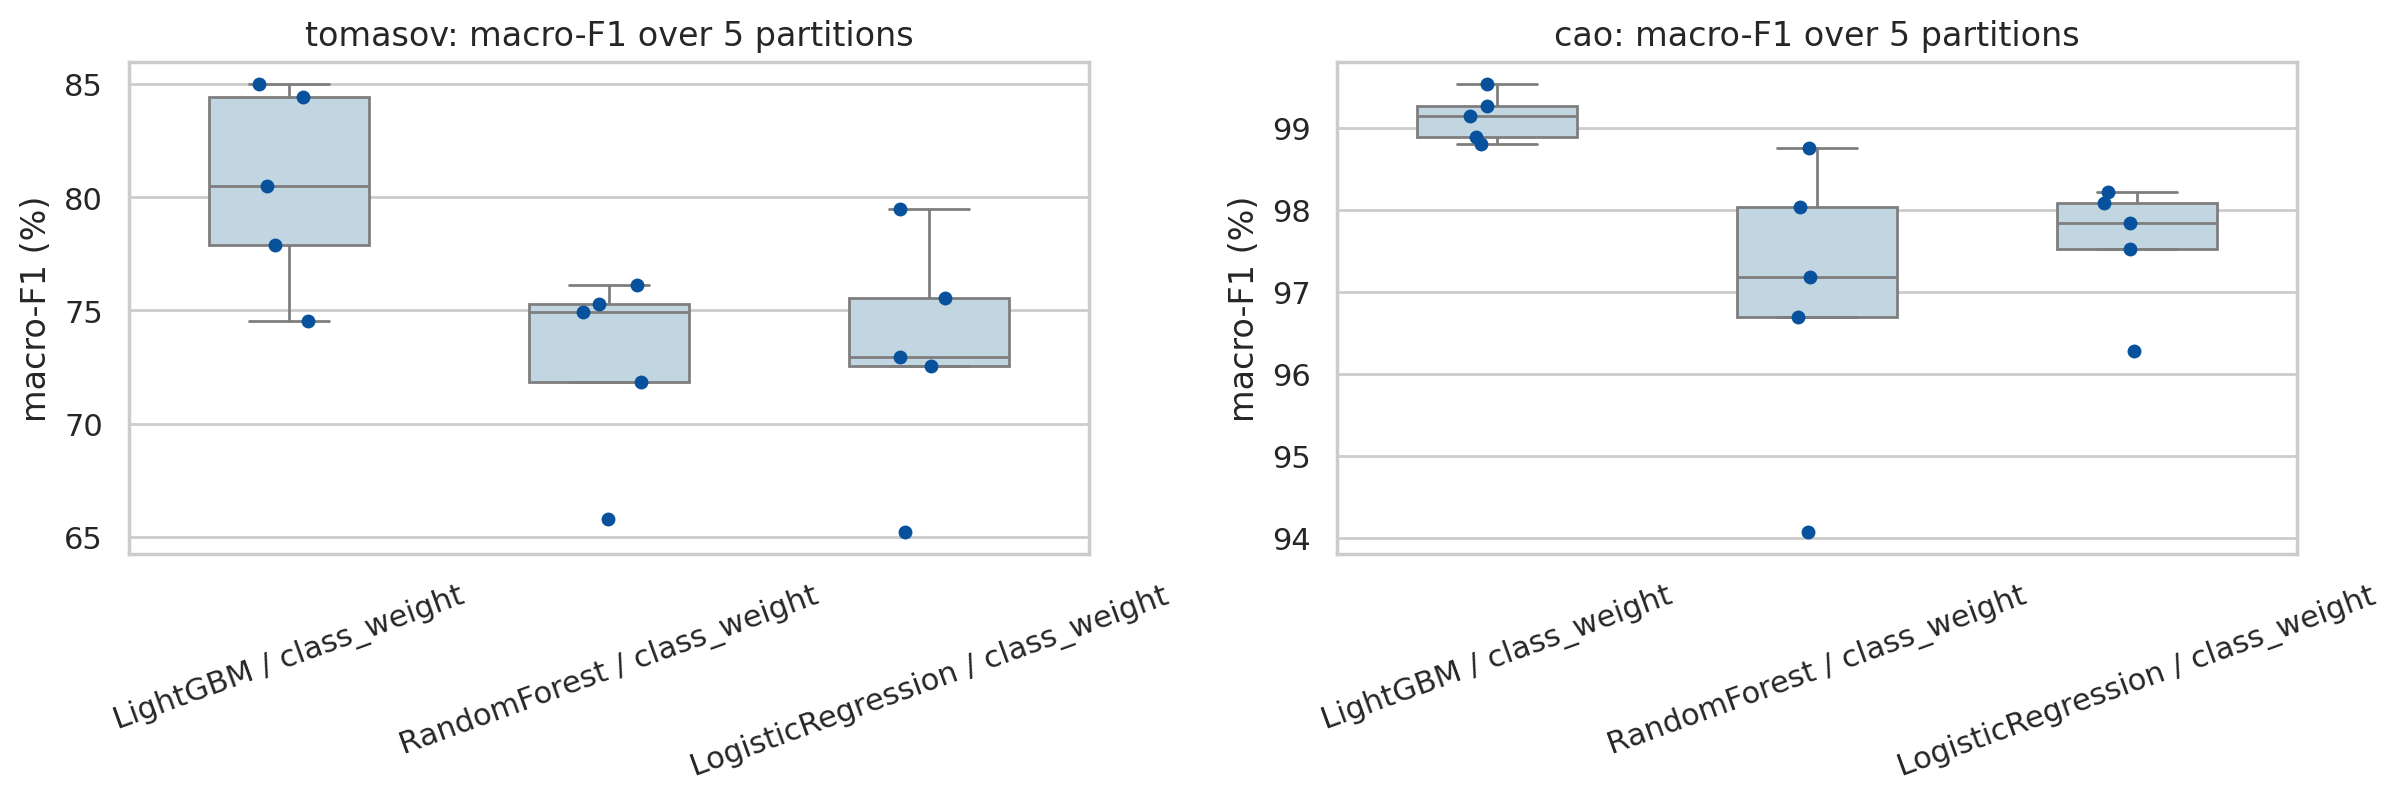
\includegraphics[width=0.95\textwidth,keepaspectratio]{Figures/fig36_repeated_splits.png}
\caption{Test macro-$F_1$ over five independently generated leakage-controlled partitions for three classifiers with class weighting: Tomasov (left) and Cao (right).}
\label{fig:repeated_splits}
\end{figure}

\paragraph[Group Bootstrap Intervals]{Group Bootstrap Intervals.}
Bootstrapping the reported test set over whole acquisitions rather than individual windows widens the $95\%$ interval by an order of magnitude on Tomasov: the interval on accuracy increases from $\pm 0.53$ at window level to $\pm 5.89$ by zone and $\pm 7.58$ by recording (\reff{fig:bootstrap_ci}). On Cao the interval changes only marginally ($\pm 0.42$ to $\pm 0.52$ by date), which indicates that the Cao acquisitions are homogeneous in accuracy whereas the Tomasov recordings are not. Window-level intervals treat overlapping windows as independent observations; as a result, they understate the uncertainty and are quoted only for comparison. Macro-$F_1$ is not estimable at the coarser levels on Tomasov, because a resample of thirteen recordings routinely omits entire classes; accuracy is therefore reported at recording level and macro-$F_1$ at zone level.

\begin{figure}[!htbp]
\centering
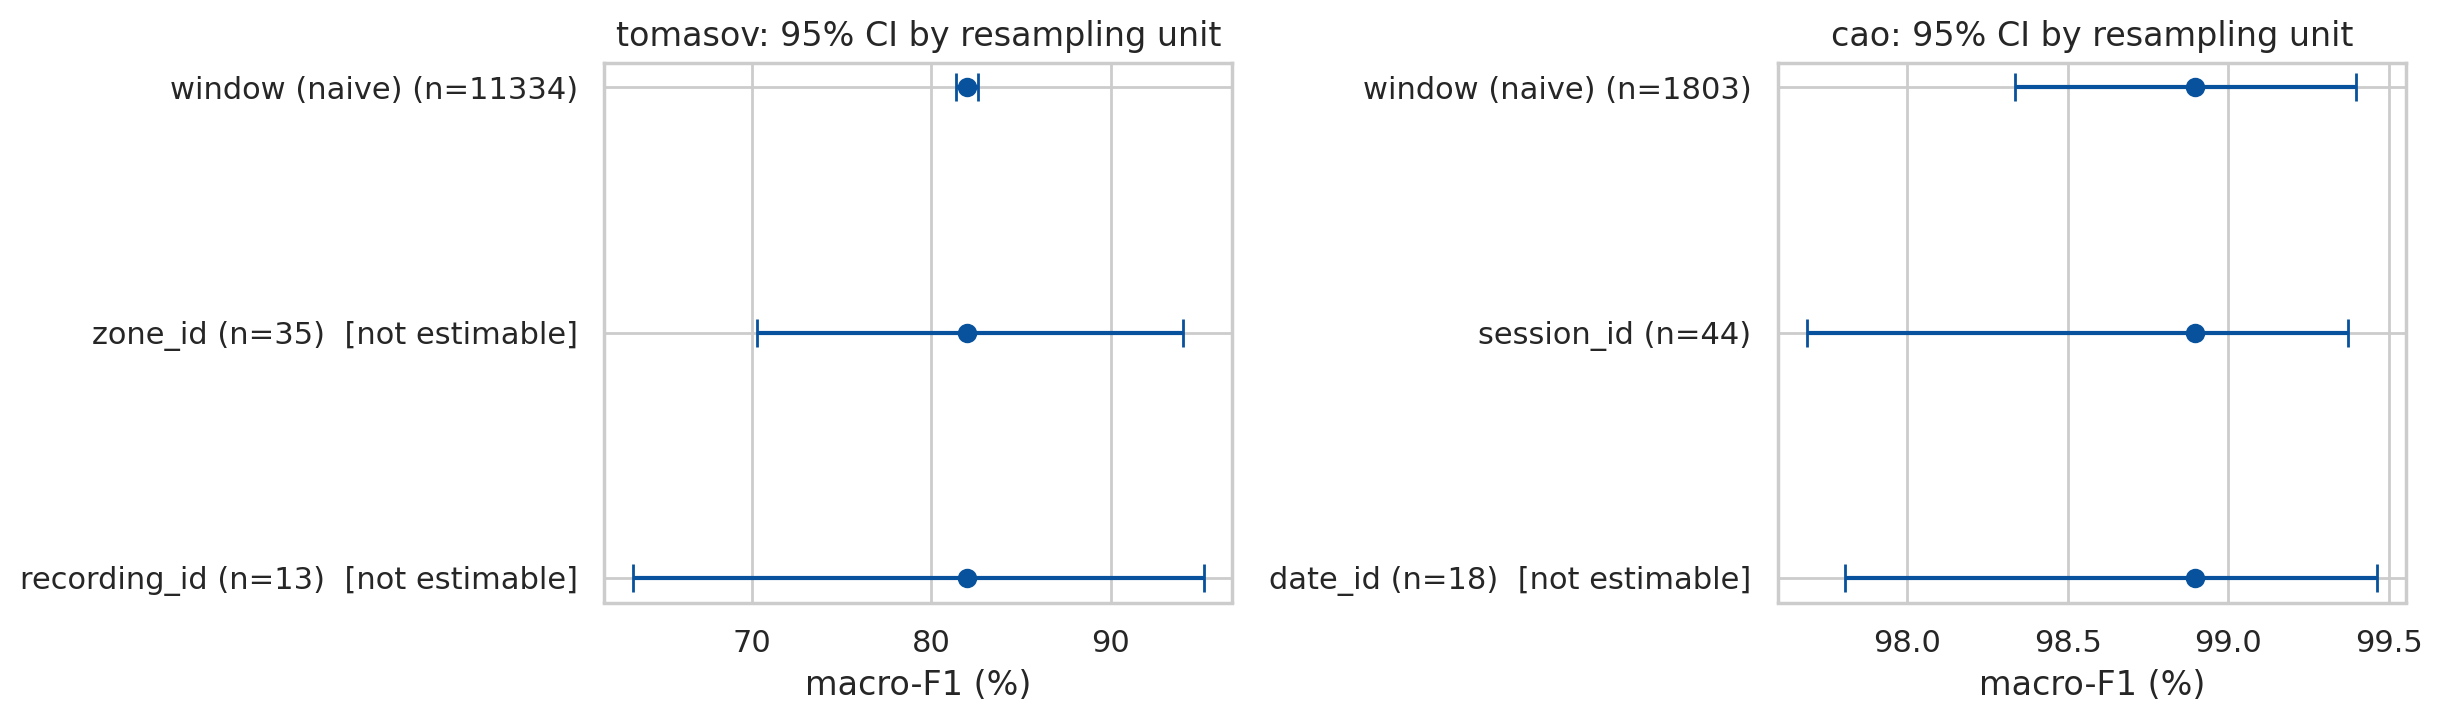
\includegraphics[width=0.95\textwidth,keepaspectratio]{Figures/fig37_group_bootstrap_ci.png}
\caption{$95\%$ bootstrap confidence intervals on test macro-$F_1$ by resampling unit: Tomasov (left) and Cao (right). Intervals marked not estimable are those in which resamples routinely omit entire classes.}
\label{fig:bootstrap_ci}
\end{figure}

\paragraph[Paired Comparison over Independent Acquisitions]{Paired Comparison over Independent Acquisitions.}
The six balancing strategies were compared again with each block consisting of a whole held-out acquisition, the model being trained on all the others, and with Holm correction across the family of pairwise comparisons~\cite{holm1979simple,demsar2006statistical}. On Tomasov, eleven held-out recordings distinguish two pairs: undersampling exceeds class weighting by $5.13$ points (corrected $p = 0.041$), and Borderline-SMOTE exceeds it by $1.44$ points (corrected $p = 0.029$). On Cao, ten held-out dates distinguish no pair of strategies on either metric (smallest corrected $p = 0.82$; the six strategies span $0.45$ accuracy points). The choice of strategy therefore has a modest effect on Tomasov and no detectable effect on Cao, in contrast to the uniform significance that the Friedman test had reported.

\section{Spatial-Domain Confound Analysis}
\label{sec:resConfound}
\autoBookmark{sec}{Spatial-Domain Confound Analysis}
High scores do not in themselves reveal what a model has learnt, and this section examines whether the measured performance reflects the events or the recordings in which they were captured. \refs{sec:resDomains} showed that 61 spatial features outperform 739 time--frequency features on Tomasov, which reverses the ordering reported in earlier single-dataset work. Spatial descriptors summarise fibre geometry, coupling, and the channel-to-channel energy structure, all of which are largely fixed within a recording, and five of the nine Tomasov classes each originate from a single recording. Part of the observed performance may therefore be attributable to recording identification rather than to event discrimination. The diagnostics of \refss{sec:chap3ConfoundDesign} test this possibility directly.

\subsection{Leave-One-Domain-Out Ablation}
\label{sec:resLODO}
\autoBookmark{subsec}{Leave-One-Domain-Out Ablation}
With the model and balancing strategy fixed at LightGBM with class weighting, so that only the feature set varies, removing the spatial block reduces macro-$F_1$ by $19.67$ points on Tomasov ($81.81$ to $62.13$) and by $5.14$ on Cao ($98.89$ to $93.75$). Removing any other domain reduces the Tomasov score by less than $0.3$ points (\reff{fig:domain_removal}). The spatial features therefore carry information that the other three domains cannot replace, whereas each of the other domains is largely redundant given the remainder. This asymmetry is the reason why the spatial domain warrants scrutiny: if its contribution were recording identity rather than event information, the Tomasov headline figure would overstate the performance that a deployment could achieve.

\begin{figure}[!htbp]
\centering
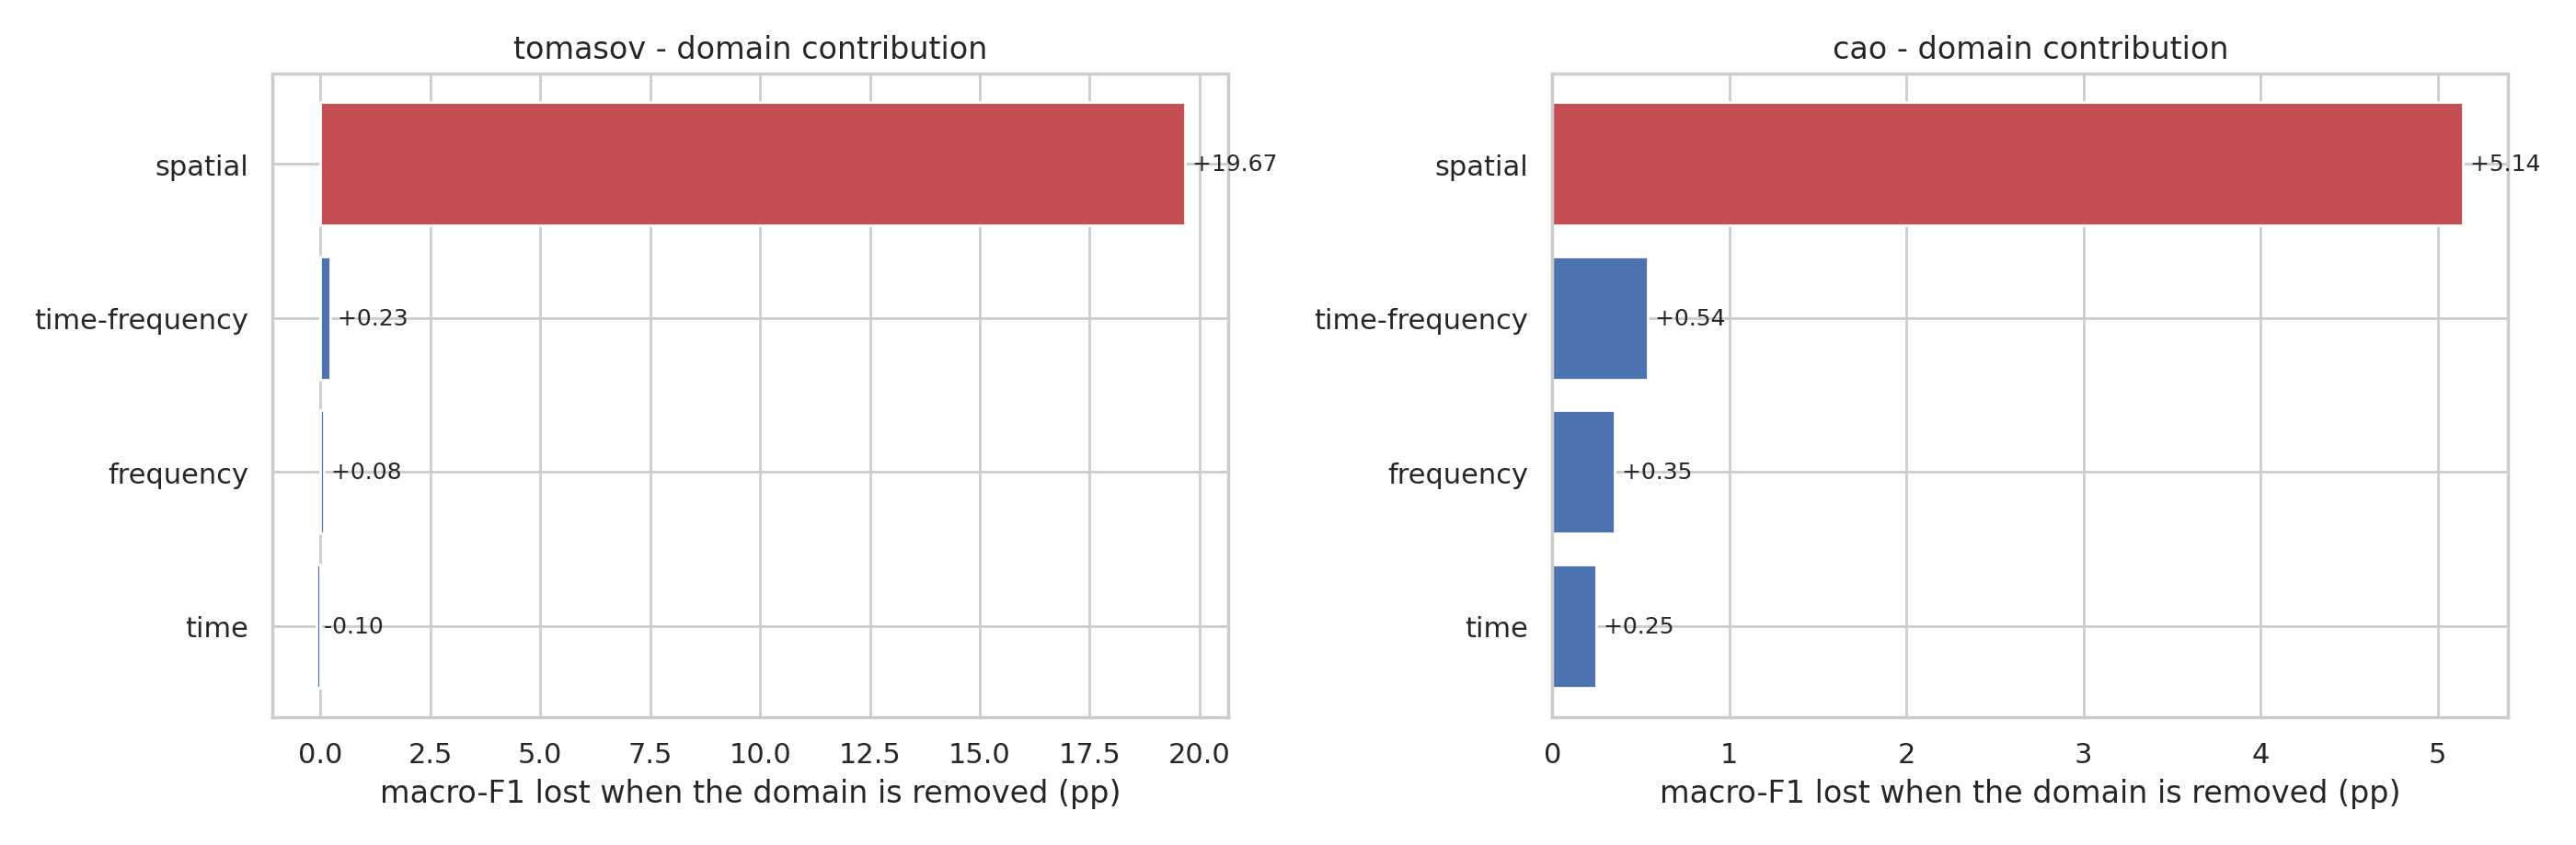
\includegraphics[width=0.9\textwidth,keepaspectratio]{Figures/fig21_domain_removal.png}
\caption{Macro-$F_1$ lost when each domain is removed from the fused representation.}
\label{fig:domain_removal}
\end{figure}

\subsection{Recording-Identity Probe}
\label{sec:resProbe}
\autoBookmark{subsec}{Recording-Identity Probe}
\reff{fig:recording_probe} presents the result of holding the event class fixed and using each domain to predict the source recording. On Tomasov, spatial features identify the recording $12.9$ points above chance, $11.1$ points more than the strongest alternative domain ($1.8$). On the \emph{car} class alone, spatial descriptors attain a recording-identification accuracy of $97.2\%$, whereas the time, frequency, and time--frequency domains remain within $0.4$ points of the majority baseline or fall below it. The spatial descriptors therefore act, at least in part, as a fingerprint of the recording in which an event was captured.

\begin{figure}[!htbp]
\centering
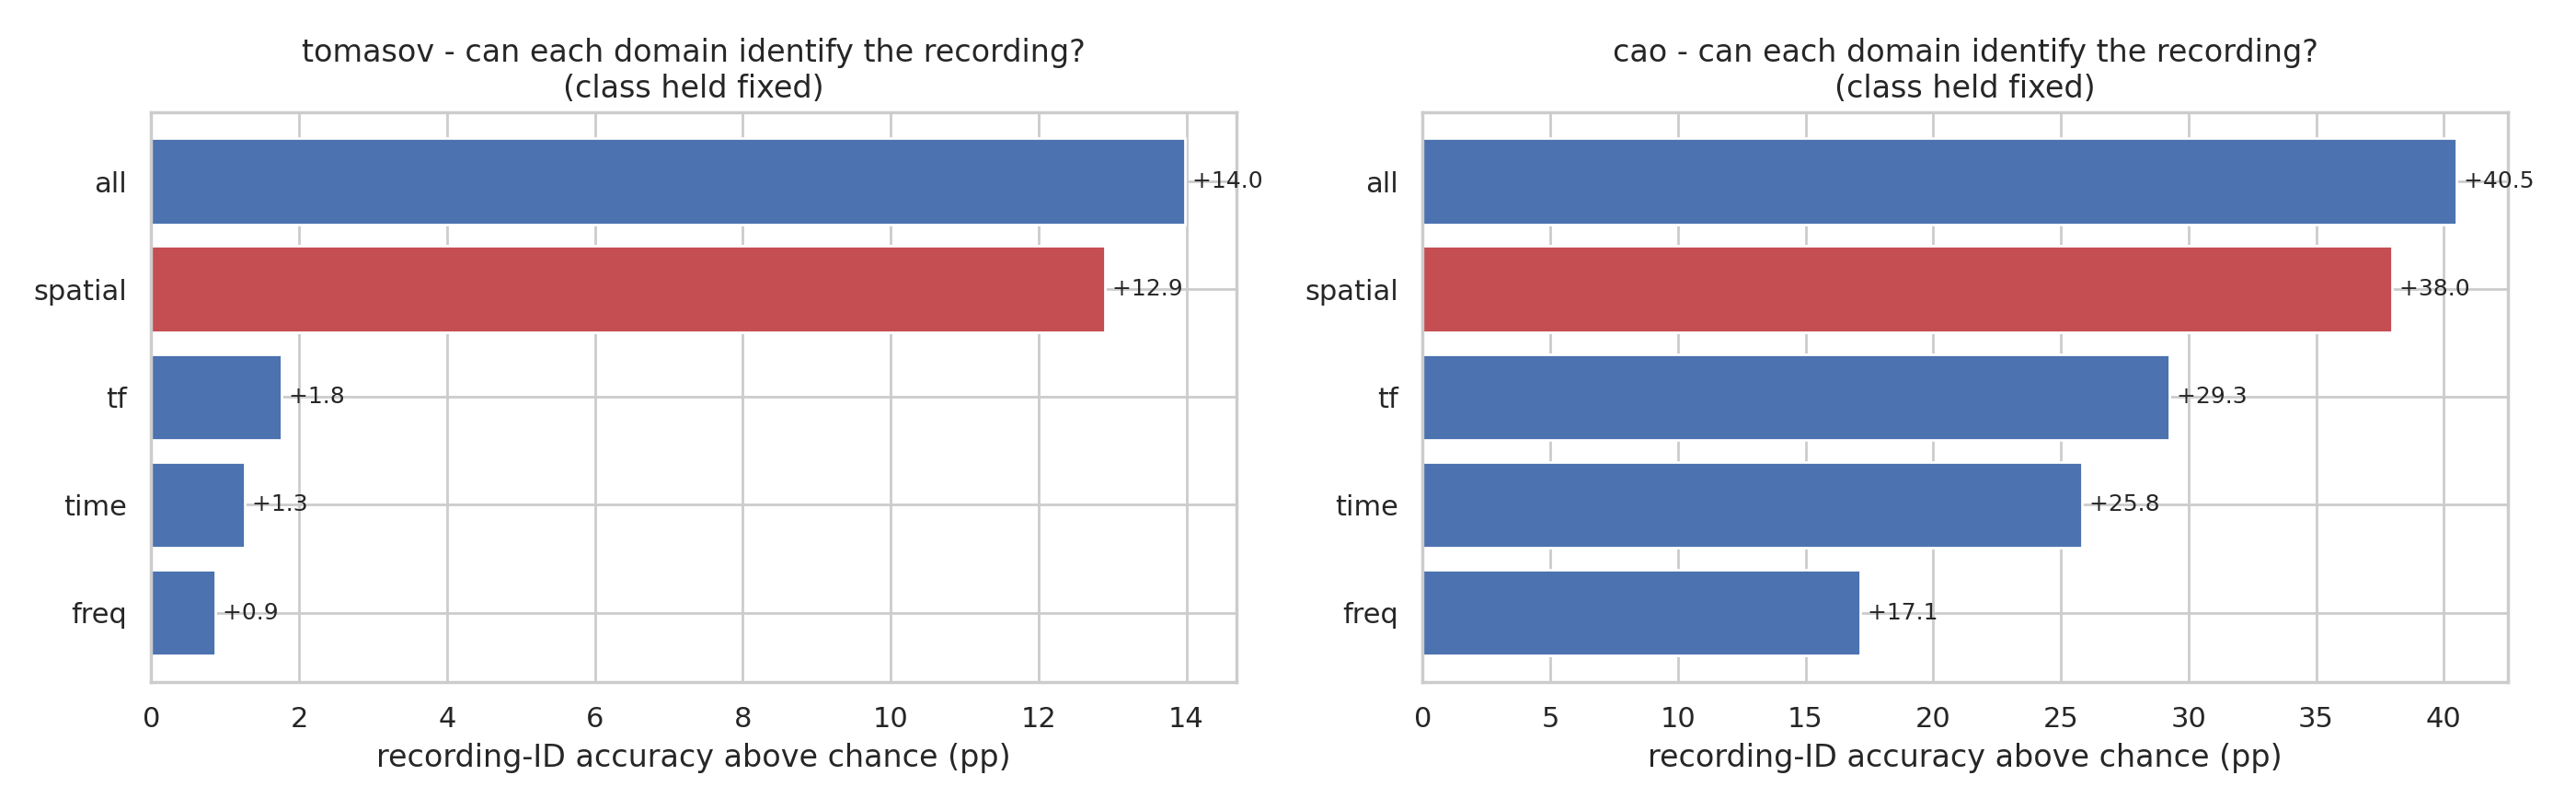
\includegraphics[width=0.9\textwidth,keepaspectratio]{Figures/fig22_recording_probe.png}
\caption{Recording-identification accuracy above chance, by feature domain, with the event class held fixed.}
\label{fig:recording_probe}
\end{figure}

\subsection{Leave-One-Recording-Out Evaluation}
\label{sec:resLORO}
\autoBookmark{subsec}{Leave-One-Recording-Out Evaluation}
The spatial features are not purely recording-specific, however. Under leave-one-recording-out evaluation, removing them reduces cross-recording accuracy by $19.08$ points on average, and only 4 of the 11 held-out recordings improve (\reff{fig:loro_spatial}). If the spatial block were purely a fingerprint, discarding it could not degrade generalisation to a recording whose fingerprint was never available during training. The motion and propagation descriptors plausibly capture physical characteristics of the events: a passing vehicle traces a spatial-centroid trajectory that remains informative across recordings.

\begin{figure}[!htbp]
\centering
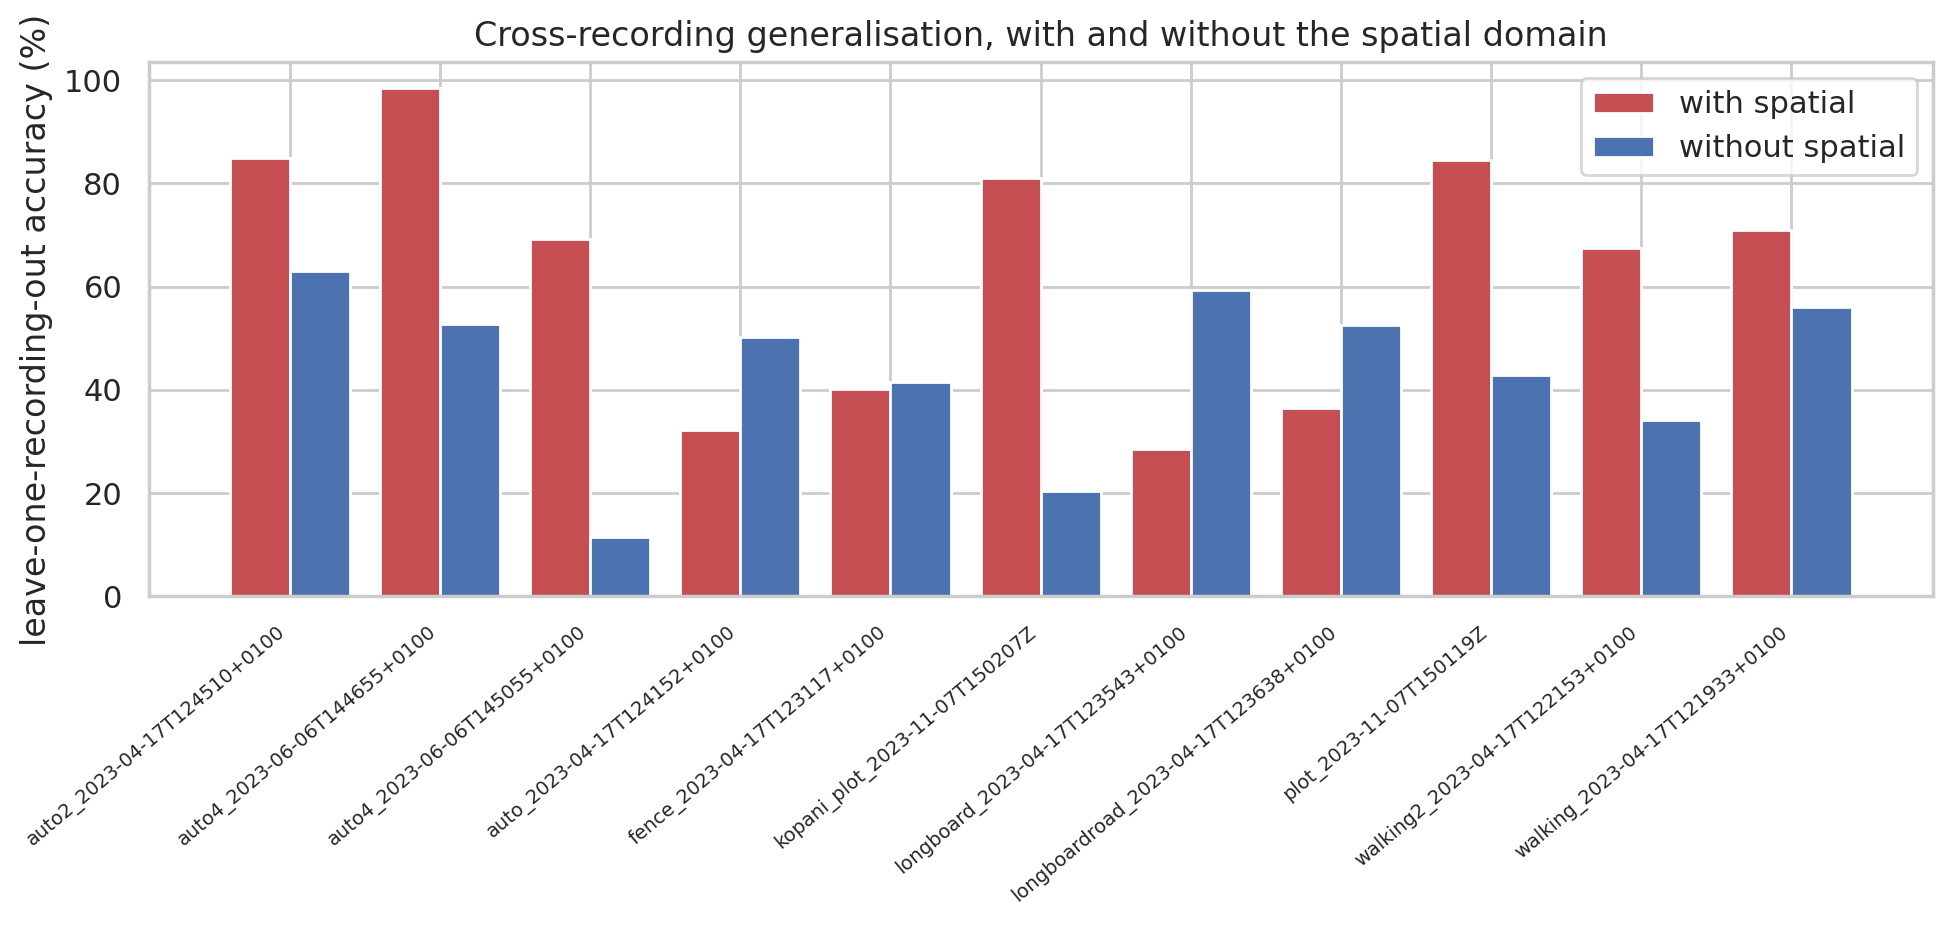
\includegraphics[width=0.9\textwidth,keepaspectratio]{Figures/fig23_loro_spatial.png}
\caption{Leave-one-recording-out accuracy with and without the spatial domain. The wide per-recording range of the difference ($-60.7$ to $+30.8$ points) indicates a mixture of transferable and recording-specific information.}
\label{fig:loro_spatial}
\end{figure}

\subsection{Implications for Reporting}
\label{sec:resConfoundVerdict}
\autoBookmark{subsec}{Implications for Reporting}
Spatial descriptors carry both transferable propagation information and recording-specific variation, and this dataset cannot separate the two, because for five of the nine classes the recording and the class are the same variable. Two figures are therefore reported for Tomasov. Where deployment recordings are represented in training, the selected configuration of Table~\ref{tab:main_results} reaches a macro-$F_1$ of $81.98$ with all features. Where they are not, a conservative figure of $62.13$ is reported, obtained by removing the spatial block. That figure is taken from the leave-one-domain-out ablation, whose all-feature reference under the same fixed configuration is $81.81$, so the cost attributable to the spatial descriptors is $19.67$ points rather than the $19.85$ that a comparison with Table~\ref{tab:main_results} would suggest.

The Cao dataset yields a different diagnosis. On this dataset the spatial margin is $8.7$ points, but every domain identifies the acquisition date well above chance ($38.0$ points for the spatial domain and $29.3$ for the strongest alternative). The confound is therefore not specific to the spatial domain but is a dataset-wide campaign confound: the entire feature space encodes acquisition conditions, which explains the decline in cross-campaign performance reported in \refs{sec:resGeneralisation}. The \emph{openclose} comparison of \refss{sec:resOpenclose} bounds the cost of aggregation over the channel axis, since a model that retains that axis recovers a class that the pooled descriptors cannot. Taken together, these findings show that the recording confound cannot be removed by partitioning alone, and they motivate the stricter generalisation tests that follow. \reff{fig:feature_importance} shows the importance distribution of the final Tomasov model by domain.

\begin{figure}[!htbp]
\centering
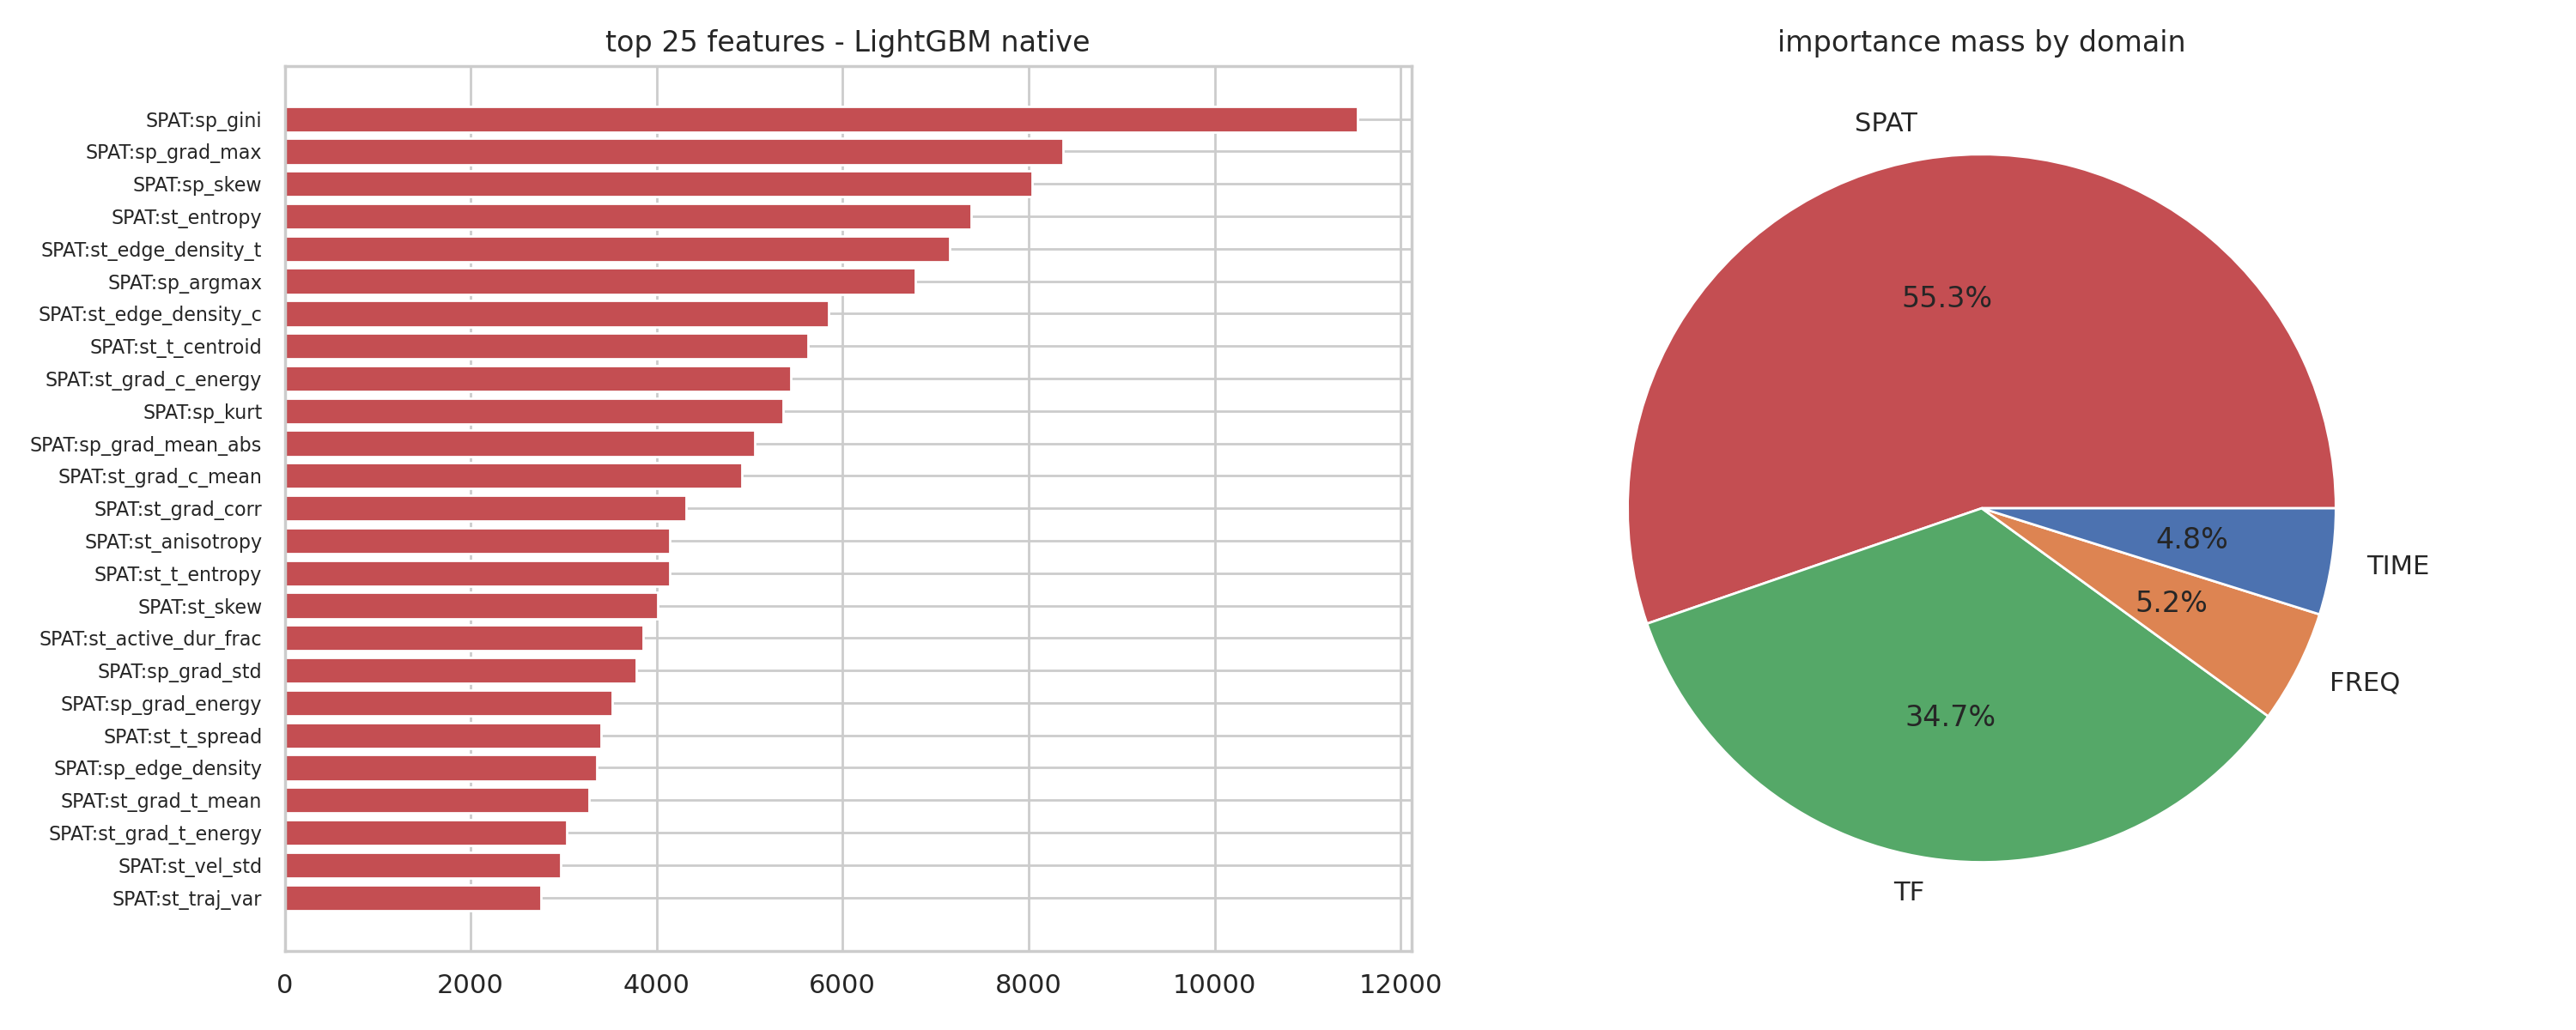
\includegraphics[width=0.95\textwidth,keepaspectratio]{Figures/fig26_feature_importance.png}
\caption{Feature importance for the final Tomasov model, coloured by domain.}
\label{fig:feature_importance}
\end{figure}

\section{Generalisation Evaluation}
\label{sec:resGeneralisationAll}
\autoBookmark{sec}{Generalisation Evaluation}
The partitions of \refs{sec:resLeakage} measure generalisation to unseen segments of recordings that are represented in training, which is a weaker requirement than generalisation to new acquisitions. This section and the next apply the stricter protocols of \refss{sec:chap3ConfoundDesign}. \refss{sec:resGeneralisation} holds out whole recordings and acquisition dates, and \refss{sec:resConsistency} examines whether the pipeline behaves consistently on the two systems. \refs{sec:resMapping} then maps the two event taxonomies onto each other and transfers a fitted model directly from one system to the other.

\subsection{Cross-Recording and Cross-Campaign Evaluation}
\label{sec:resGeneralisation}
\autoBookmark{subsec}{Cross-Recording and Cross-Campaign Evaluation}
On the four Tomasov classes recorded more than once, leave-one-recording-out accuracy averages $63.85\%$ (SD $29.31$), compared with $90.71\%$ within represented recordings, a reduction of $26.86$ points when generalising to an unseen recording. The per-recording range is wide, from $6.22\%$ to $99.05\%$ across the eleven held-out recordings, and the mean should therefore not be interpreted as a stable operating point.

On Cao, leave-one-date-out evaluation reduces accuracy from $99.06\%$ to $86.81\%$, with a range of $48.84\%$ to $100.00\%$ across the ten dates. The macro-$F_1$ figure requires careful interpretation and is not quoted. Every held-out date contains fewer than the six classes, and six of them contain only two, while macro-$F_1$ averaged over the union of true and predicted labels scores each absent class as zero: date 220113 combines $98.56\%$ accuracy with a macro-$F_1$ of $49.62$. The degradation is genuine but concentrated. Eight of the ten dates exceed $84\%$ accuracy, while two (220517 and 220518) fall below $52\%$; acquisition identity therefore remains a substantial source of variation, although a smaller one than an uncorrected macro-$F_1$ would suggest. Table~\ref{tab:generalisation} summarises both evaluations.

\begin{table}[!htbp]
	\centering
	\caption{Generalisation under progressively stricter protocols. Acc.: accuracy. Macro-$F_1$ is omitted where held-out units do not contain every class.}
	\label{tab:generalisation}
	\small
	\begin{tabular}{@{}lrrr@{}}
		\toprule
		\textbf{Evaluation} & \textbf{Classes} & \textbf{Acc. (\%)} & \textbf{Macro-$F_1$}\\
		\midrule
		Tomasov, blocked split             & 9 & 90.71 & 81.98\\
		Tomasov, leave-one-recording-out   & 4 & \textbf{63.85} & ---\\
		\midrule
		Cao, session-grouped               & 6 & 99.06 & 98.90\\
		Cao, leave-one-date-out            & 6 & \textbf{86.81} & ---\\
		\bottomrule
	\end{tabular}
\end{table}

\subsection{Consistency of Feature Behaviour Across the Two Systems}
\label{sec:resConsistency}
\autoBookmark{subsec}{Consistency of Feature Behaviour Across the Two Systems}
When the same pipeline is applied to both datasets, feature-domain performance correlates at $\rho = 0.90$ and per-feature selection rates at $\rho = 0.55$. Five features are selected unanimously on both: the minimum, lower quartile, and range of the STFT temporal envelope, the maximum spectral flux, and the Gini coefficient of the segment energies. Given the differences in sensing principle, interrogator, channel spacing, sampling rate, and taxonomy, this agreement is evidence that parts of the behaviour of the pipeline transfer between acquisition systems. The agreement is strong at the level of domains and moderate at the level of individual features, which is the pattern expected when two systems observe related physical phenomena at different spatial resolutions. Whether a model fitted on one system can classify the events of the other is a more demanding question, which is addressed in the next section.

\section{Mapping Between the Tomasov and Cao Event Taxonomies}
\label{sec:resMapping}
\autoBookmark{sec}{Mapping Between the Tomasov and Cao Event Taxonomies}
The two datasets were annotated by different groups for different purposes, and their taxonomies share only one label name, \emph{walk}. A test of whether a fitted model generalises from one system to the other therefore requires a mapping between their event classes that is based on the physical mechanism at the fibre rather than on the label names. This section presents that mapping (\refss{sec:resMappingTable}), reports the performance of the pipeline on the classes that the two datasets share (\refss{sec:resMappingWithin}), trains on one system and tests on the other (\refss{sec:resTransfer}), and considers the implications of the outcome for generalisability (\refss{sec:resMappingVerdict}). \refss{sec:chap3Mapping} describes the procedure.

\subsection{Correspondence Between the Event Classes}
\label{sec:resMappingTable}
\autoBookmark{subsec}{Correspondence Between the Event Classes}
\reff{fig:label_mapping} and Table~\ref{tab:label_mapping} present the correspondence. Four of the nine Tomasov classes and four of the six Cao classes map one-to-one onto a shared event type. \emph{Background} pairs the Tomasov \emph{regular} class, routine activity along the fibre route with no target event, with the Cao recordings in which no deliberate event takes place. \emph{Walk} pairs the only label that the two taxonomies already share. \emph{Impact} pairs the Tomasov \emph{fence} class, in which the fence beside the buried cable is struck or kicked, with the Cao \emph{knocking} class; both deliver short impulsive strikes that reach the fibre through a structure or the ground. \emph{Excavation} pairs the Tomasov \emph{construction} class with the Cao \emph{digging} class. Both disturb the ground near the cable, although at very different scales, namely construction machinery compared with manual digging.

\begin{figure}[!htbp]
\centering
\setstretch{1}%
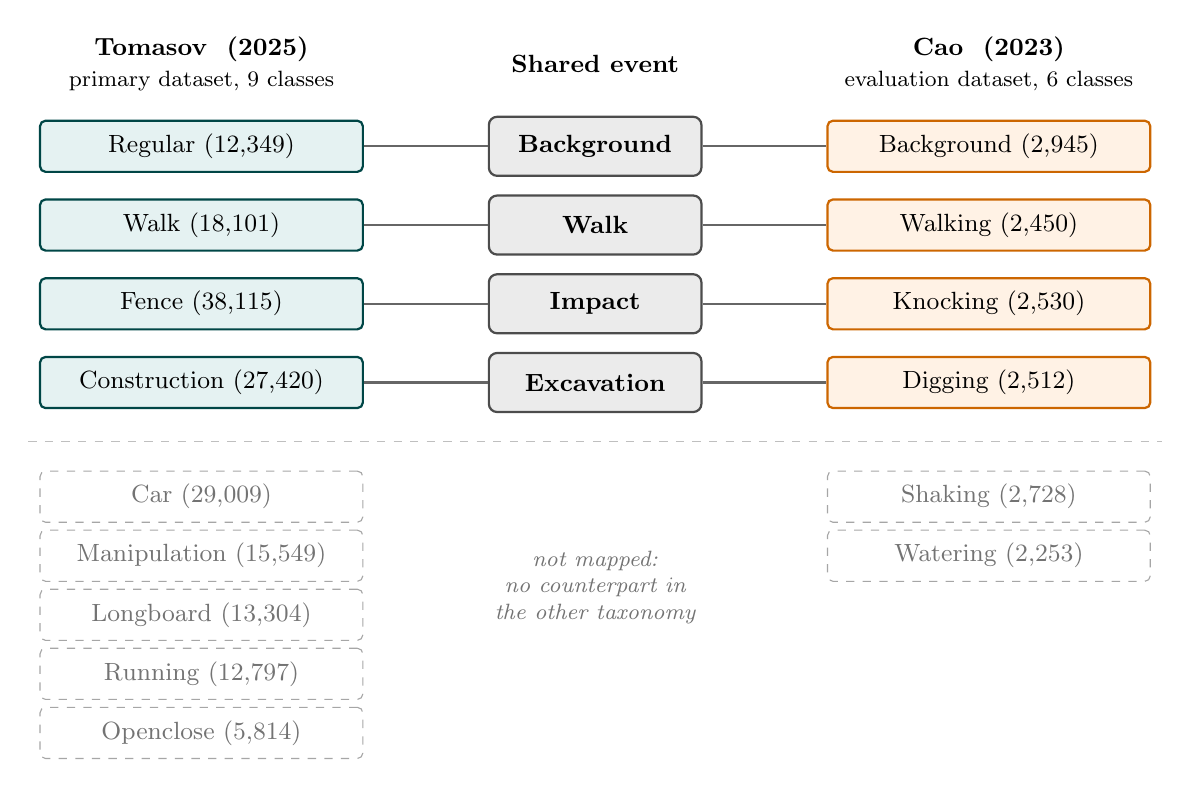
\begin{tikzpicture}[
	font=\small,
	cls/.style={rounded corners=2pt, minimum width=4.1cm, minimum height=6.5mm, inner sep=2pt, align=center, thick},
	tomC/.style={cls, draw=teal!55!black, fill=teal!10},
	caoC/.style={cls, draw=orange!80!black, fill=orange!10},
	harm/.style={draw=black!70, fill=black!8, thick, rounded corners=3pt, minimum width=2.7cm, minimum height=7.5mm, font=\small\bfseries},
	off/.style={cls, thin, draw=black!35, dashed, text=black!55, fill=white},
	link/.style={thick, black!60},
	hdr/.style={font=\small\bfseries, align=center},
]
\foreach \y/\t/\h/\c [count=\i] in {0/Regular (12{,}349)/Background/Background (2{,}945), -1/Walk (18{,}101)/Walk/Walking (2{,}450), -2/Fence (38{,}115)/Impact/Knocking (2{,}530), -3/Construction (27{,}420)/Excavation/Digging (2{,}512)} {
	\node[tomC] (t\i) at (0,\y) {\t};
	\node[harm] (h\i) at (5,\y) {\h};
	\node[caoC] (c\i) at (10,\y) {\c};
	\draw[link] (t\i.east) -- (h\i.west);
	\draw[link] (h\i.east) -- (c\i.west);
}
\draw[black!25, dashed] (-2.2,-3.75) -- (12.2,-3.75);
\foreach \y/\t [count=\i] in {-4.45/Car (29{,}009), -5.2/Manipulation (15{,}549), -5.95/Longboard (13{,}304), -6.7/Running (12{,}797), -7.45/Openclose (5{,}814)} {
	\node[off] (tu\i) at (0,\y) {\t};
}
\foreach \y/\t [count=\i] in {-4.45/Shaking (2{,}728), -5.2/Watering (2{,}253)} {
	\node[off] (cu\i) at (10,\y) {\t};
}
\node[font=\footnotesize\itshape, text=black!55, align=center] at (5,-5.6) {not mapped:\\no counterpart in\\the other taxonomy};
\node[hdr] at (0,1.05) {Tomasov \etal\ (2025)\\{\footnotesize\normalfont primary dataset, 9 classes}};
\node[hdr] at (5,1.05) {Shared event};
\node[hdr] at (10,1.05) {Cao \etal\ (2023)\\{\footnotesize\normalfont evaluation dataset, 6 classes}};
\end{tikzpicture}
\caption{Mapping between the Tomasov and Cao event taxonomies. Four classes on each side map one-to-one onto a shared event type; the remaining classes (dashed) have no counterpart and are excluded from the cross-system tests. Numbers in brackets are Tomasov windows in the final partition and Cao records.}
\label{fig:label_mapping}
\end{figure}

\begin{table}[!htbp]
	\centering
	\caption{Shared event types of the Tomasov and Cao datasets, the physical mechanism behind each, and the samples each covers. Tomasov counts are windows in the final partition; Cao counts are records.}
	\label{tab:label_mapping}
	\small
	\setlength{\tabcolsep}{4pt}
	\begin{tabularx}{\textwidth}{@{}l >{\raggedright\arraybackslash}X l r l r@{}}
		\toprule
		\textbf{Shared event} & \textbf{Mechanism at the fibre} & \textbf{Tomasov} & \textbf{Windows} & \textbf{Cao} & \textbf{Records}\\
		\midrule
		Background  & Ambient state, no target event & Regular      & 12{,}349 & Background & 2{,}945\\
		Walk        & Pedestrian footfall & Walk         & 18{,}101 & Walking    & 2{,}450\\
		Impact      & Impulsive strikes through a structure or the ground & Fence        & 38{,}115 & Knocking   & 2{,}530\\
		Excavation  & Ground worked by machinery or tools & Construction & 27{,}420 & Digging    & 2{,}512\\
		\midrule
		Mapped      & & 4 of 9 classes & 95{,}985 & 4 of 6 classes & 10{,}437\\
		Not mapped  & & 5 classes      & 76{,}473 & 2 classes      & 4{,}981\\
		\bottomrule
	\end{tabularx}
\end{table}

The mapping covers $95{,}985$ of the $172{,}458$ Tomasov windows ($55.7\%$) and $10{,}437$ of the $15{,}418$ Cao records ($67.7\%$). Seven classes are excluded. \emph{Car} and \emph{longboard} are vehicle events with no Cao counterpart. \emph{Running} also consists of footfall, but merging it into \emph{walk} would alter the composition of a class that already has a direct counterpart, for which reason it was excluded rather than merged. \emph{Manipulation} and \emph{openclose} describe interference with the installation at a manhole on the route, for which the Cao setup has no equivalent, and the Cao classes \emph{shaking} and \emph{watering} have no equivalent among the Tomasov classes.

\subsection{Performance on the Shared Classes}
\label{sec:resMappingWithin}
\autoBookmark{subsec}{Performance on the Shared Classes}
Restricting each dataset to its four mapped classes provides a within-system reference (Table~\ref{tab:transfer}). Using only the 941 non-spatial features, LightGBM trained on the $81{,}645$ Tomasov training windows of the four classes and tested on the $6{,}987$ test windows of the frozen partition reaches $73.02\%$ accuracy and a macro-$F_1$ of $70.01$. On Cao, with $7{,}888$ training and $1{,}451$ test records, it reaches $95.93\%$ and $94.45$. The Tomasov reference is lower than the nine-class headline because the spatial block is excluded: without it the nine-class macro-$F_1$ falls to $62.13$ (\refss{sec:resLODO}), and the four shared classes, at $70.01$, lie between the two values. Within each system, the shared events can thus be recognised from signal-agnostic features alone, which is the precondition for a meaningful transfer test.

\subsection{Cross-System Transfer}
\label{sec:resTransfer}
\autoBookmark{subsec}{Cross-System Transfer}
Training on every mapped window of one system and testing on every mapped window of the other yields accuracies below the $25\%$ chance level in both directions: $14.41\%$ when the model is trained on Cao and tested on Tomasov, and $19.12\%$ in the reverse direction (Table~\ref{tab:transfer}). Balanced accuracy, at $21.66\%$ and $20.02\%$, is likewise below chance, which shows that the failure is not an artefact of the class proportions.

\begin{table}[!htbp]
	\centering
	\caption{Within-system and cross-system performance on the four shared event types, using the 941 time, frequency, and time--frequency features. Chance accuracy is $25\%$.}
	\label{tab:transfer}
	\small
	\begin{tabular}{@{}lrrrrr@{}}
		\toprule
		\textbf{Training $\rightarrow$ test} & \textbf{Train} & \textbf{Test} & \textbf{Acc. (\%)} & \textbf{Bal. acc. (\%)} & \textbf{Macro-$F_1$}\\
		\midrule
		Tomasov $\rightarrow$ Tomasov (within) & 81{,}645 & 6{,}987  & 73.02 & 69.29 & 70.01\\
		Cao $\rightarrow$ Cao (within)         & 7{,}888  & 1{,}451  & 95.93 & 94.57 & 94.45\\
		\midrule
		Cao $\rightarrow$ Tomasov              & 10{,}437 & 95{,}985 & 14.41 & 21.66 & 12.97\\
		Tomasov $\rightarrow$ Cao              & 95{,}985 & 10{,}437 & 19.12 & 20.02 & 15.99\\
		\bottomrule
	\end{tabular}
\end{table}

\reff{fig:cross_system} shows the manner in which the transferred models fail. When trained on Cao, the model assigns most Tomasov windows of every class to \emph{background} (from $59.8\%$ of true background to $78.0\%$ of true excavation) and never predicts \emph{impact}, so its recall is $59.8\%$ on background, $17.1\%$ on excavation, $9.7\%$ on walk, and zero on impact. When trained on Tomasov, the model assigns most Cao records to \emph{impact} or \emph{walk}: $80.5\%$ of background records are classified as impact, and $79.0\%$ of excavation and $71.5\%$ of impact records are classified as walk. It never predicts \emph{background}, and its highest recall is $47.1\%$ on walk. Each model collapses the data of the other system onto one or two of its own classes, which is characteristic of a covariate shift so large that the feature distributions of the two systems scarcely overlap even after quantile normalisation.

\begin{figure}[!htbp]
\centering
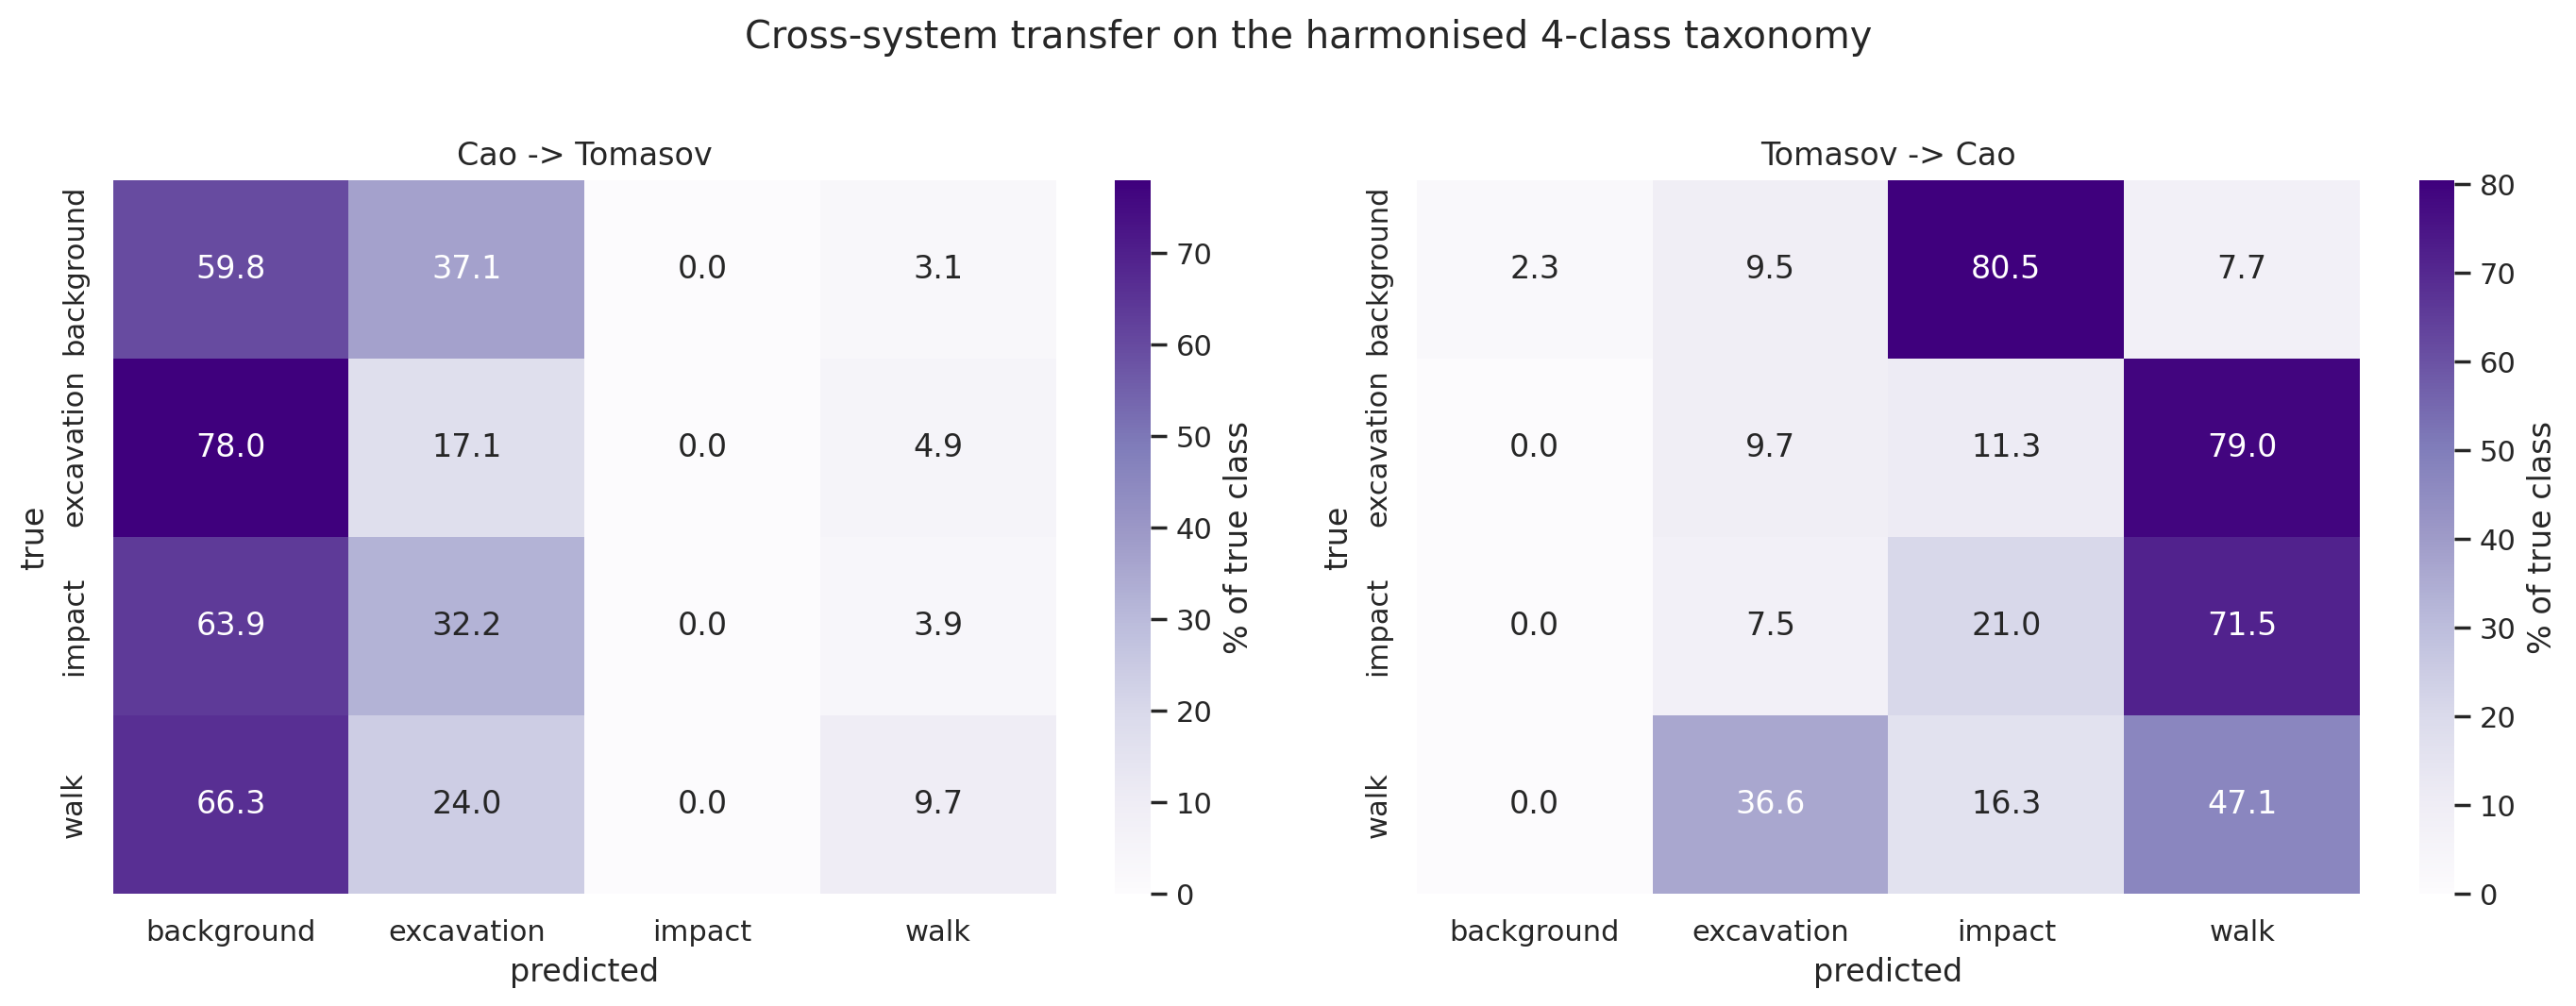
\includegraphics[width=0.95\textwidth,keepaspectratio]{Figures/fig35_cross_system_confusion.png}
\caption{Row-normalised confusion matrices for direct cross-system transfer on the four shared event types: trained on Cao and tested on Tomasov (left), and trained on Tomasov and tested on Cao (right).}
\label{fig:cross_system}
\end{figure}

\subsection{Implications of the Mapping for Generalisability}
\label{sec:resMappingVerdict}
\autoBookmark{subsec}{Implications of the Mapping for Generalisability}
The mapping converts an imprecise question, whether the pipeline generalises across DAS systems, into a measurable one, and the answer depends on the sense in which generalisation is understood. The pipeline as a method transfers: the same configuration, without per-dataset tuning, recognises the shared events well within each system, ranks the feature domains almost identically on both ($\rho = 0.90$), and outperforms the baselines on both (\refs{sec:resDiscussion}). A fitted model does not transfer: when trained on one system, it performs below chance on the other. Two explanations cannot be distinguished with these data. The shared event types may not be physically equivalent across the two installations (construction machinery and manual digging differ greatly in energy and duration, and a fence strike reaches the cable through a different path from a knock on the ground), or the intensity-based and phase-sensitive interrogators may record the same disturbance so differently that quantile normalisation cannot align them. In either case, the deployment of a fitted model on a new interrogator requires labelled data from that interrogator or explicit domain adaptation; adaptation is a prerequisite rather than a refinement. The mapping also provides future work with an established benchmark, since any adaptation method can be evaluated on exactly these four classes in both directions. This negative result completes the generalisation part of \textbf{RQ3}.

\section{Computational Efficiency and Lightweight Footprint}
\label{sec:resEfficiency}
\autoBookmark{sec}{Computational Efficiency and Lightweight Footprint}
Computational cost determines whether the workflow can be executed at the location where a DAS system is deployed, and this section answers \textbf{RQ1}. \refss{sec:resRealTime} decomposes the per-window cost of the pipeline into its stages and compares it with the real-time budget, and \refss{sec:resFootprint} compares the complete footprint of the pipeline with that of every baseline, using the four measures of \refss{sec:chap3Efficiency}.

\subsection{Per-Window Cost and the Real-Time Budget}
\label{sec:resRealTime}
\autoBookmark{subsec}{Per-Window Cost and the Real-Time Budget}
Table~\ref{tab:efficiency} separates the stages of the per-window online cost, measured on the CPU of the Jetson AGX Orin. Classifier inference is sub-millisecond on both datasets and negligible in relation to the window-arrival interval. Feature extraction dominates the cost, and within it the time--frequency domain accounts for approximately $60$\,ms per window, owing to the wavelet-packet decomposition over 16 sub-bands and the grey-level co-occurrence computation. For Tomasov, the total of $144.59$\,ms exceeds the window-arrival interval of $102.4$\,ms, and two cores are consequently required for real-time processing of a single channel. For Cao, the total of $122.54$\,ms fits within the interval of $204.8$\,ms on one core. Feature selection is a one-time offline cost; Boruta is the most expensive method at $665$\,s (Tomasov) and $745$\,s (Cao), and the filter methods complete in under five seconds. Preprocessing is negligible relative to extraction, as anticipated in \refss{sec:chap3PreprocCost}.

\begin{table}[!htbp]
	\centering
	\caption{Computational cost per window and the real-time budget.}
	\label{tab:efficiency}
	\small
	\begin{tabular}{@{}lrr@{}}
		\toprule
		\textbf{Stage} & \textbf{Tomasov (ms)} & \textbf{Cao (ms)}\\
		\midrule
		Time-domain extraction        & 43.16 & 42.62\\
		Frequency-domain extraction   & 3.35  & 3.34\\
		Time--frequency extraction    & 60.67 & 59.49\\
		Spatial extraction            & 37.40 & 17.10\\
		\midrule
		\textbf{Total extraction}     & \textbf{144.59} & \textbf{122.54}\\
		Classifier inference          & 0.17  & 0.06\\
		\midrule
		Window arrival interval       & 102.4 & 204.8\\
		Cores required for real time  & 2     & 1\\
		\bottomrule
	\end{tabular}
\end{table}

\subsection{Lightweight Footprint of the Pipeline and the Baselines}
\label{sec:resFootprint}
\autoBookmark{subsec}{Lightweight Footprint of the Pipeline and the Baselines}
Table~\ref{tab:footprint} compares the four footprint measures of the pipeline with those of the two published CNNs and the five recent architectures, all trained on the same leakage-controlled partitions and timed on the same board. The feature pipeline runs on the CPU cores of the board, whereas every network was trained and executed on its integrated GPU. The two LightGBM sizes are obtained by counting the split thresholds, split features, and leaf values of the fitted boosters, and refitting the selected configurations under the fixed seed reproduces their reported test metrics exactly. The native text model file of LightGBM, which also stores split gains and node counts, is larger: $32.8$\,MB on Tomasov and $8.5$\,MB on Cao, or $14.7$ and $3.5$\,MB when compressed.

\begin{table}[!htbp]
	\centering
	\caption[Lightweight footprint of the pipeline and every baseline]{Lightweight footprint of the feature pipeline and every baseline on the Jetson AGX Orin, on the leakage-controlled partitions. Size counts stored parameters at 32 bits each (\refss{sec:chap3Efficiency}). Latencies are per window and amortised over the test set; end-to-end latency adds the preparation of each model's input. n.r.: not recorded.}
	\label{tab:footprint}
	\footnotesize
	\setlength{\tabcolsep}{3.5pt}
	\resizebox{\textwidth}{!}{%
	\begin{tabular}{@{}llrrrrr@{}}
		\toprule
		\textbf{Model} & \textbf{Processor} & \textbf{Parameters} & \textbf{Size (MB)} & \textbf{Training (s)} & \textbf{Inference (ms)} & \textbf{End-to-end (ms)}\\
		\midrule
		\multicolumn{7}{@{}l}{\textit{Tomasov \etal\ 2025}}\\[2pt]
		Pipeline, $1{,}002$ feat.\ (proposed) & CPU & 855{,}000 & 3.42 & 1{,}357 & 0.17 & 144.77\\
		Pipeline, 52 feat.\ (proposed) & CPU & 855{,}000 & 3.42 & \textbf{63} & 0.15 & 144.74$^{a}$\\
		Tomasov CNN, dense 1024~\cite{tomasov2025perimeter} & GPU & 33{,}155{,}849 & 132.62 & 1{,}569 & n.r. & n.r.\\
		Tomasov CNN, dense 256~\cite{tomasov2025perimeter}  & GPU & 8{,}375{,}561 & 33.50 & 1{,}103 & n.r. & n.r.\\
		DAStatFormer~\cite{dione2026dastatformer} & GPU & 16{,}077{,}327 & 64.31 & 32{,}958 & 0.62 & $\geq 0.62^{b}$\\
		DASViT1D~\cite{dione2025intrusion}        & GPU & 1{,}655{,}561 & 6.62 & 1{,}184 & \textbf{0.16} & $\geq 0.16^{b}$\\
		S2-DyGNN~\cite{jeong2026s2dygnn}          & GPU & 56{,}329 & 0.23 & 25{,}530 & 5.67 & 5.67\\
		GAT~\cite{jeong2026s2dygnn,shahabudin2024gnn} & GPU & 52{,}361 & 0.21 & 25{,}135 & 5.08 & 5.08\\
		GCN~\cite{jeong2026s2dygnn,shahabudin2024gnn} & GPU & 48{,}137 & \textbf{0.19} & 37{,}704 & 5.16 & 5.16\\
		\midrule
		\multicolumn{7}{@{}l}{\textit{Cao \etal\ 2023}}\\[2pt]
		Pipeline, $1{,}002$ feat.\ (proposed) & CPU & 208{,}578 & 0.83 & 41 & \textbf{0.06} & 122.60\\
		Pipeline, 53 feat.\ (proposed) & CPU & 357{,}390 & 1.43 & \textbf{8} & 0.07 & 122.61$^{a}$\\
		Cao CNN~\cite{caoxin2023opendataset} & GPU & 7{,}421 & \textbf{0.03} & 628 & n.r. & n.r.\\
		DAStatFormer~\cite{dione2026dastatformer} & GPU & 15{,}985{,}164 & 63.94 & 1{,}775 & 0.76 & $\geq 0.76^{b}$\\
		DASViT1D~\cite{dione2025intrusion}        & GPU & 1{,}655{,}174 & 6.62 & 130 & 0.19 & $\geq 0.19^{b}$\\
		S2-DyGNN~\cite{jeong2026s2dygnn}          & GPU & 56{,}134 & 0.22 & 1{,}392 & 3.75 & 3.75\\
		GAT~\cite{jeong2026s2dygnn,shahabudin2024gnn} & GPU & 52{,}166 & 0.21 & 2{,}063 & 3.10 & 3.10\\
		GCN~\cite{jeong2026s2dygnn,shahabudin2024gnn} & GPU & 47{,}942 & 0.19 & 2{,}531 & 3.03 & 3.03\\
		\bottomrule
	\end{tabular}}
	\par\smallskip
	\begin{minipage}{\textwidth}\scriptsize
	Pipeline: LightGBM on the full or the consensus feature set. $^{a}$\,The extractor computes every domain in full, so the consensus configuration pays the full extraction cost. $^{b}$\,Excludes computing the model's input features (MFCC, RDFT, and DWT for DASViT1D; 24 statistics per channel for DAStatFormer), which were computed in advance and not timed. The graph models compute their STFT inside the timed forward pass, so their figure is end-to-end apart from the band-pass and z-score conditioning they share with the pipeline.
	\end{minipage}
\end{table}

The four measures rank the models differently, which is the reason why all four are required. In \emph{model size}, the $3.42$\,MB of the pipeline on Tomasov is a nineteenth of the size of DAStatFormer ($64.31$\,MB), a tenth to a thirty-ninth of that of the reconstructed Tomasov CNN ($33.50$--$132.62$\,MB), and half of that of DASViT1D ($6.62$\,MB), but fifteen to eighteen times the size of the three graph networks, each of which holds about fifty thousand weights; on Cao the same ordering holds at $0.83$\,MB, with the $7{,}421$-weight Cao CNN the smallest model overall. In \emph{inference latency}, the CPU classifier of the pipeline ($0.17$ and $0.06$\,ms) matches the fastest network on its GPU, DASViT1D, on Tomasov ($0.16$\,ms) and is three times faster on Cao ($0.19$\,ms); it is four to twelve times faster than DAStatFormer and thirty to sixty times faster than the graph networks. In \emph{training cost}, the pipeline requires $1{,}357$\,s on Tomasov and $41$\,s on Cao on CPU cores, against $1{,}103$--$37{,}704$\,s and $130$--$2{,}531$\,s of GPU time for the networks; only DASViT1D and the smaller Tomasov CNN train faster on Tomasov, and the consensus configuration trains in $63$ and $8$\,s, faster than every network on both datasets. In \emph{end-to-end latency}, the order is reversed. Feature extraction brings the online cost of the pipeline to $122.60$--$144.77$\,ms per window, compared with $3.03$--$5.67$\,ms for the graph networks, and the cost of computing the input features of the transformers was not timed.

These measurements answer RQ1. A DAS classifier is lightweight in the sense of \refs{sec:ResearchBackground} when its learning stage is small, requires no GPU, and trains within minutes, and when its complete online cost fits within the window-arrival interval on a few CPU cores of the board located beside the interrogator. The feature pipeline satisfies that definition: a model of $0.8$--$3.4$\,MB, CPU-only training in under $23$ minutes (about one minute with consensus selection), sub-millisecond CPU inference, and an online cost that fits within the window interval on one core for Cao and two for Tomasov. It is not, however, the lightest model on every measure. The graph networks are smaller and, given a GPU, less costly per window, but each requires seven to ten and a half hours of GPU training on Tomasov, and their decisions cannot be traced to named quantities (\refss{sec:resWhiteBox}). The lightness of the pipeline therefore lies in its learning stage and its hardware requirements, and its most expensive component is feature extraction, in which further savings should be sought (\refss{sec:chap5FutureCost}). Real-time claims based on inference latency alone would omit that principal online cost, and for this reason the end-to-end figure is reported for every model.
\section{Discussion}
\label{sec:resDiscussion}
\autoBookmark{sec}{Discussion}
This section relates the preceding results to the prior work on which they build. The baseline branch of \reff{fig:methodology_framework} trains the CNN published with each dataset and five recent architectures on raw windows, or on the input features their designs compute from them, drawn from the same partitions as the feature pipeline, and scores them with the same metrics on the same test windows, so that every difference reported in this section is attributable to the models and the evaluation protocols rather than to the data. The aim is to establish how, and why, the findings of this study differ from the accuracies reported in the source publications. \refss{sec:resCNN} compares the pipeline with the published CNNs; \refss{sec:resCapacity} and \refss{sec:resReproGap} use those networks to measure the sensitivity of a single architecture to leakage; \refss{sec:resSOTA} extends the comparison to five architectures published from 2024 onwards, with the size and latency of every model; \refss{sec:resWhiteBox} contrasts the white-box pipeline with the black-box networks; and \refss{sec:resSynthesis} synthesises the comparisons.

\subsection{Comparison with the Published CNN Baselines}
\label{sec:resCNN}
\autoBookmark{subsec}{Comparison with the Published CNN Baselines}
Table~\ref{tab:cnn_comparison} compares the feature pipeline with the CNN published with each dataset, trained on identical leakage-controlled partitions as specified in \refss{sec:chap3Baselines}. The pipeline leads by $16.43$ macro-$F_1$ points on Tomasov and $8.01$ on Cao, which answers the comparative part of \textbf{RQ3} for the published baselines. The partitions are identical across models, but the inputs are not: the feature pipeline operates on demeaned, band-passed, z-scored windows, whereas each CNN is reproduced on the raw records that its source publication assumes. Under the operational rates defined with the Cao dataset, its CNN attains a nuisance-alarm rate of $0.45\%$ and a false-negative rate of $0.89\%$ on the session-grouped partition; equivalent rates were not computed for the feature pipeline and are not claimed.

\begin{table}[!htbp]
	\centering
	\caption[Feature pipeline compared with the CNN baselines]{Feature pipeline compared with the CNN baselines, and the protocol sensitivity of the reconstructed Tomasov CNN. Parameters are trainable weights for the CNNs and stored split and leaf values for LightGBM; size counts them at 32 bits each. Latency is per window on the Jetson AGX Orin, given for the pipeline as classifier inference / end-to-end including feature extraction; the CNNs' inference time was not recorded (n.r.). Acc.: accuracy; $\Delta$Acc.: change from the same model on the blocked partition.}
	\label{tab:cnn_comparison}
	\footnotesize
	\setlength{\tabcolsep}{4pt}
	\resizebox{\textwidth}{!}{%
\begin{tabular}{@{}lrrr>{\raggedright\arraybackslash}p{3.2cm}rrr@{}}
		\toprule
		\textbf{Method} & \textbf{Parameters} & \textbf{Size (MB)} & \textbf{Latency (ms)} & \textbf{Partition} & \textbf{Acc. (\%)} & \textbf{Macro-$F_1$} & \textbf{$\Delta$Acc.}\\
		\midrule
		\multicolumn{8}{@{}l@{}}{\emph{Tomasov 2025}}\\
		Multi-domain features, $1{,}002$ & 855\,k & 3.42 & 0.17 / 144.77 & Blocked + guard bands & \textbf{90.71} & \textbf{81.98} & ---\\
		Consensus features, 52           & 855\,k & 3.42 & 0.15 / 144.74 & Blocked + guard bands & 77.29 & 73.59 & ---\\
		Tomasov CNN, reconstructed, dense 1024 & 33.2\,M & 132.62 & n.r. & Blocked + guard bands & 68.74 & 65.55 & ---\\
		Tomasov CNN, reconstructed, dense 256  & 8.4\,M  & 33.50  & n.r. & Blocked + guard bands & 67.28 & 64.66 & ---\\
		\midrule
		\multicolumn{8}{@{}l@{}}{\emph{Protocol sensitivity of the reconstructed Tomasov CNN (dense 1024)}}\\
		Random partition, same windows   & 33.2\,M & 132.62 & n.r. & Random 80/10/10, 2{,}048-sample stride & 69.99 & 69.90 & $+1.25$\\
		Random partition, windows re-cut & 33.2\,M & 132.62 & n.r. & Random 80/10/10, 256-sample stride & 95.01 & 94.64 & $+26.27$\\
		Published~\cite{tomasov2025perimeter}, authors' protocol & Not stated & --- & --- & Random 10-fold, 256-sample stride & 85.47 & 84.84 & ---\\
		\midrule
		\multicolumn{8}{@{}l@{}}{\emph{Cao 2023}}\\
		Multi-domain features, $1{,}002$ & 209\,k & 0.83 & 0.06 / 122.60 & Session-grouped & \textbf{99.06} & \textbf{98.90} & ---\\
		Consensus features, 53           & 357\,k & 1.43 & 0.07 / 122.61 & Session-grouped & 94.40 & 93.08 & ---\\
		Cao CNN~\cite{caoxin2023opendataset} & 7{,}421 & 0.03 & n.r. & Session-grouped & 91.13 & 90.88 & ---\\
		\bottomrule
	\end{tabular}}
\end{table}

\begin{figure}[!htbp]
\centering
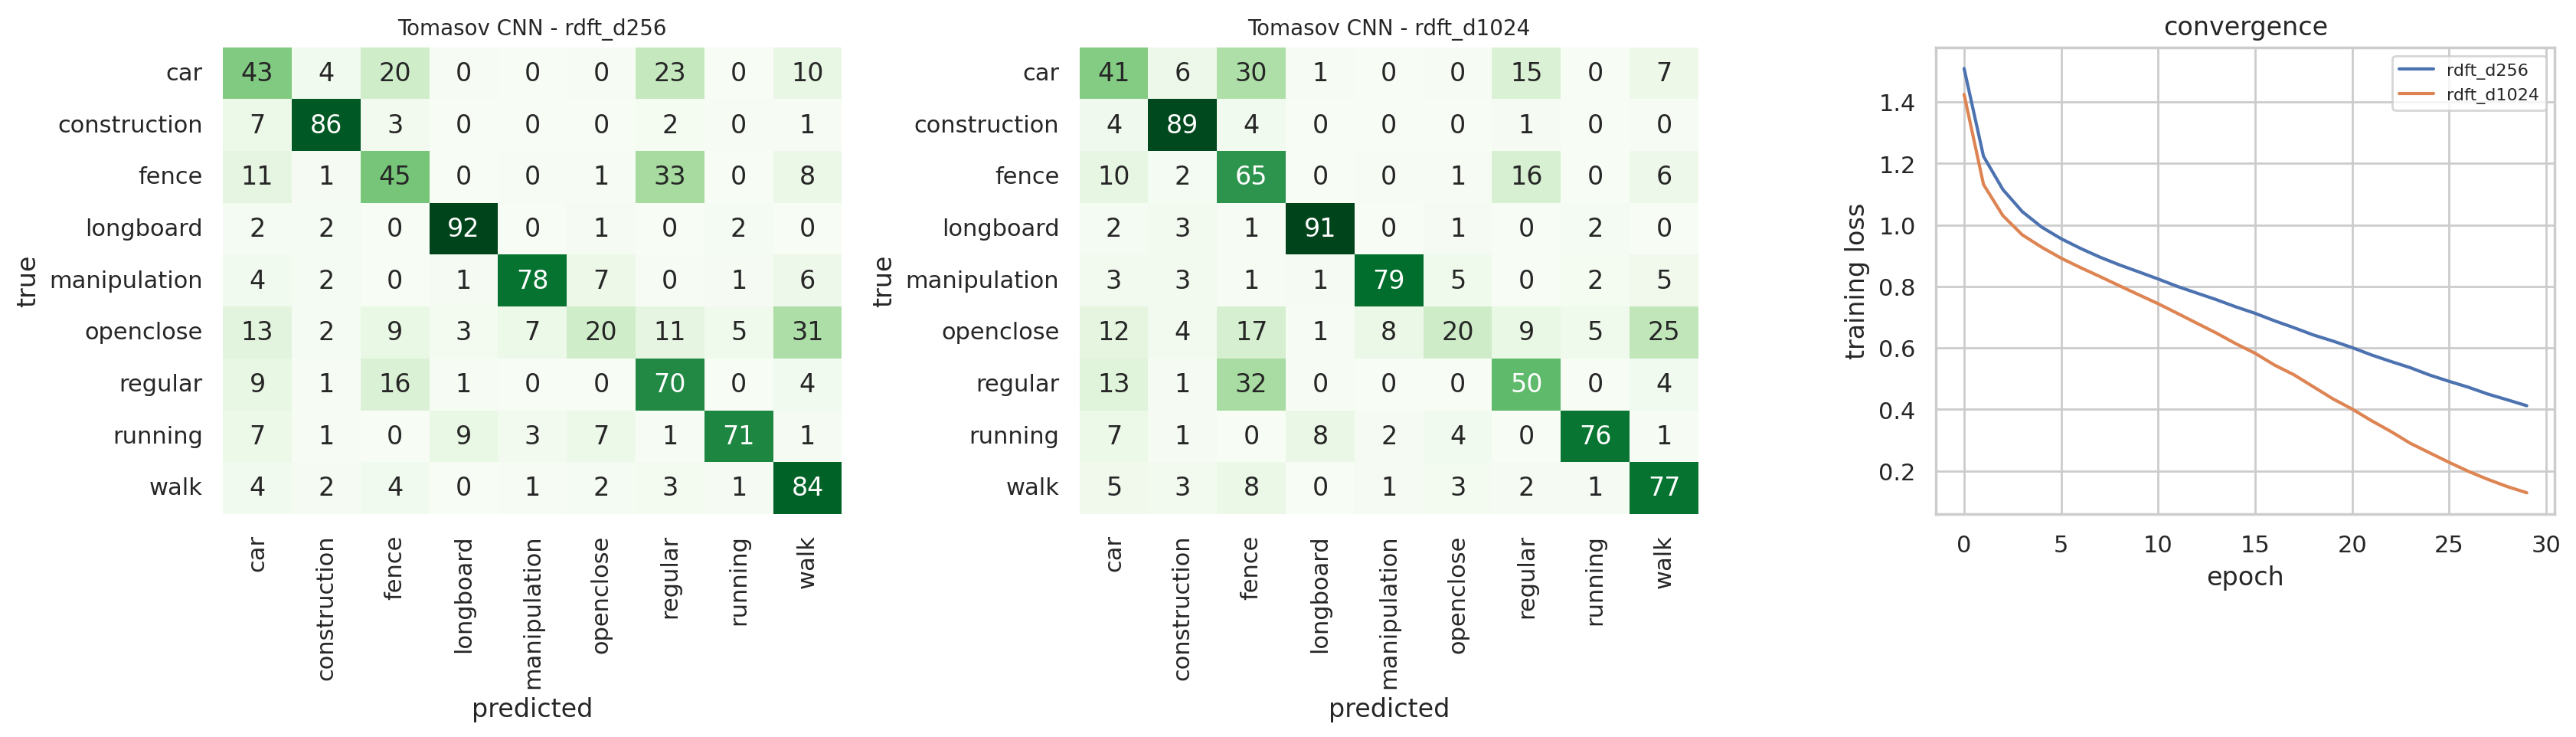
\includegraphics[width=0.98\textwidth,keepaspectratio]{Figures/fig31_tomasov_cnn.png}
\caption{Reconstructed Tomasov CNN on the blocked partition: row-normalised confusion matrices for the 256-unit and $1{,}024$-unit dense layers, and training convergence.}
\label{fig:tomasov_cnn}
\end{figure}

\subsection{Model Capacity and Leakage Sensitivity}
\label{sec:resCapacity}
\autoBookmark{subsec}{Model Capacity and Leakage Sensitivity}
The Cao CNN was trained under both its released partition and the session-grouped partition, which provides a controlled estimate of the extent to which that architecture exploits leakage. Accuracy decreases from $92.70\%$ to $91.13\%$ and macro-$F_1$ from $92.47$ to $90.88$, reductions of only $1.58$ and $1.59$ points despite the near-total contamination documented in \refs{sec:resLeakage}. \reff{fig:cao_cnn} shows the confusion matrices and convergence under both protocols.

\begin{figure}[!htbp]
\centering
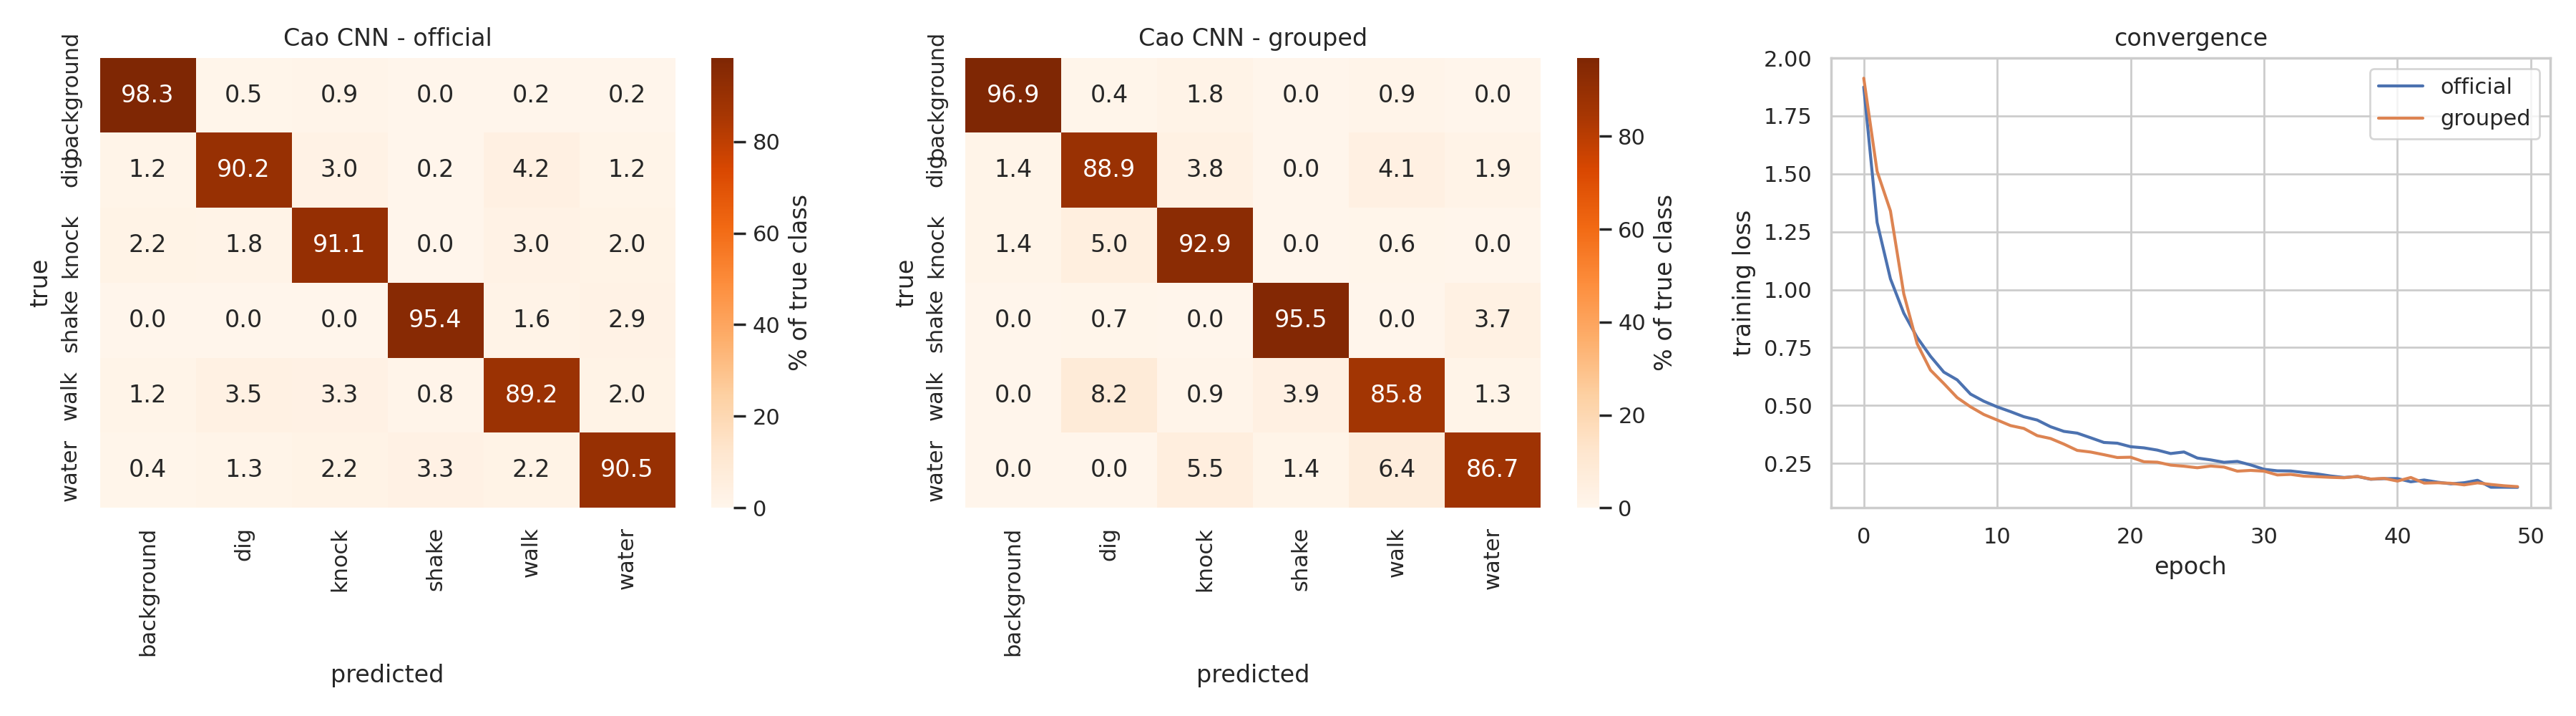
\includegraphics[width=0.95\textwidth,keepaspectratio]{Figures/fig25_cao_cnn.png}
\caption{Cao CNN under both protocols: confusion matrices and training convergence.}
\label{fig:cao_cnn}
\end{figure}

Model capacity is one plausible explanation. With $7{,}421$ parameters, this network has far less capacity than a $1{,}002$-feature gradient-boosted ensemble and may be less able to exploit recording-specific structure. On this account, leakage does not affect all models equally and may favour higher-capacity models, so model rankings obtained under contaminated protocols need not agree with rankings obtained under group-aware evaluation. \refss{sec:resSOTA} tests this hypothesis across five further architectures.

\subsection{Protocol Attribution for the Tomasov CNN}
\label{sec:resReproGap}
\autoBookmark{subsec}{Protocol Attribution for the Tomasov CNN}
The reconstructed Tomasov CNN attains $68.74\%$ accuracy under the blocked partition, compared with the $85.47\%$ reported by its authors. The attribution of that gap requires that one variable be changed at a time, and the network was accordingly trained three times with the architecture, seed, front end, and training recipe fixed and only the partition varied (\reff{fig:protocol_attribution}). Under a random partition of the same $2{,}048$-hop windows it reaches $69.99\%$, a gain of $1.25$ points. Under a random partition of windows re-cut at the 256-sample stride of the authors, which reproduces their window density, it reaches $95.01\%$: $26.27$ points above the blocked partition and $25.02$ above the random partition at the coarser stride. The protocol alone therefore accounts for $26.27$ accuracy points on an otherwise identical model, and the inflation is driven by the density of the overlap rather than by the randomness of the assignment. At $75\%$ overlap a random split adds $1.25$ points; at $96.9\%$ it adds $26.27$.

\begin{figure}[!htbp]
\centering
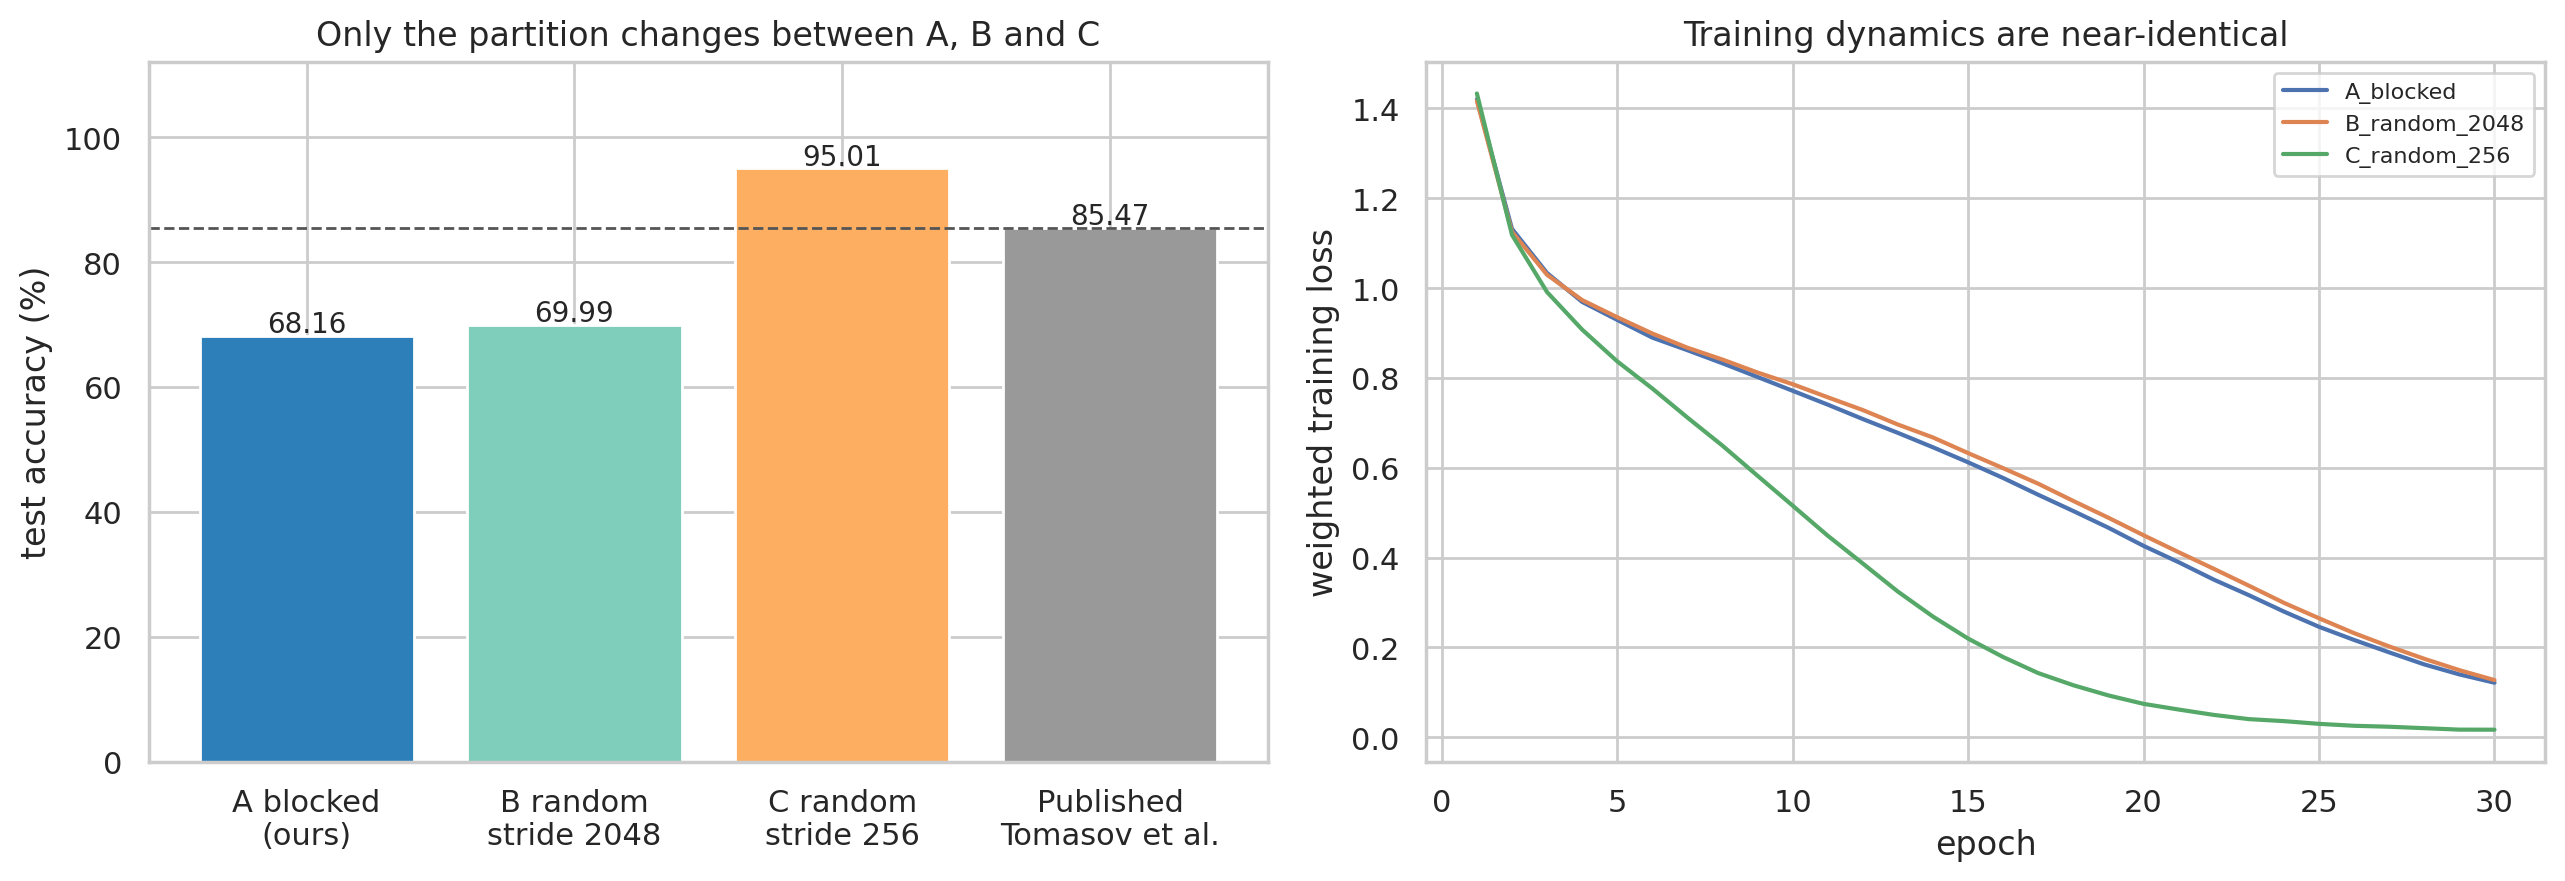
\includegraphics[width=0.98\textwidth,keepaspectratio]{Figures/fig32_protocol_attribution.png}
\caption{Protocol attribution for the reconstructed Tomasov CNN. Left: test accuracy under the three arms and the published figure; only the partition differs between arms. Right: weighted training loss per epoch, which is near-identical for arms A and B and collapses under arm C, the signature of memorised near-duplicates. The arm-A bar is from the attribution run and differs from the value in Table~\ref{tab:cnn_comparison} by a few tenths, the run-to-run variation of single CNN trainings on this dataset.}
\label{fig:protocol_attribution}
\end{figure}

The published figure of $85.47\%$ was not reproduced exactly. Under the protocol of the authors the reconstruction achieves $95.01\%$, exceeding the published figure by $9.54$ points, and this discrepancy is reported rather than removed by tuning. The excess is consistent with leakage in the re-cut windows that is at least as strong as in the originals: the final training loss is $0.017$ under arm C against $0.121$ under the leakage-controlled partition. The consequence for the comparison is favourable, but it must be stated precisely. The reconstruction is not a weakened replica, so the $68.74\%$ measured under leakage control cannot be attributed to a poor reimplementation; it is a fair measurement of that architecture under a sample-disjoint protocol. The source specifies a 256-unit dense layer, and the $1{,}024$-unit variant is reported as the reproduction because it scores higher, which means that the comparison is likewise not made against a weakened baseline. The fourfold increase in capacity yields only $0.89$ macro-$F_1$ points.

Two limitations remain. First, the re-cut partition reconstructs the published protocol rather than reproducing it, since it expands a sampled subset of parent windows onto the 256-sample grid, with the result that leakage is dense within clusters whereas the original tiling is continuous. Second, single-run CNN accuracies on this dataset should be interpreted only to the nearest point, because training runs that differ only in row ordering vary by a few tenths.

\subsection{Comparison with Recent Architectures}
\label{sec:resSOTA}
\autoBookmark{subsec}{Comparison with Recent Architectures}
Five architectures published from 2024 onwards were reimplemented and trained under the partitions, preprocessing constraints, and metrics used throughout this thesis (\refss{sec:chap3SOTA}). Table~\ref{tab:sota} reports the results, with the parameter count, stored size, and per-window latency of every model, and \reff{fig:sota} illustrates them. On Tomasov the feature pipeline attains $90.71\%$ accuracy and $81.98$ macro-$F_1$, exceeding the strongest neural baseline by $11.88$ accuracy points and $3.44$ macro-$F_1$ points. On Cao it attains $99.06\%$ and $98.90$, exceeding the strongest neural baseline by $1.11$ and $1.32$. \refss{sec:chap5LimResidue} qualifies the Tomasov margin. The ordering in the published literature is not preserved: S2-DyGNN reports $94.0\%$ accuracy on Tomasov under its own chronological partition and reaches $77.59\%$ under the present protocol, and DAStatFormer reports $99.93\%$ and reaches $78.83\%$.

\begin{table}[!htbp]
	\centering
	\caption[Recent architectures under the leakage-controlled protocol]{Recent architectures under the leakage-controlled protocol, with the size and latency of each model. All models use identical partitions, preprocessing constraints, and metrics. Size counts stored parameters at 32 bits each; latency is per window on the Jetson AGX Orin (CPU for the pipeline, GPU for the networks), given for the pipeline as classifier inference / end-to-end including feature extraction. Published accuracy is each method's own reported figure under its own protocol. Table~\ref{tab:footprint} adds training cost.}
	\label{tab:sota}
	\footnotesize
	\setlength{\tabcolsep}{4pt}
	\resizebox{\textwidth}{!}{%
\begin{tabular}{@{}lrrrrrrrr@{}}
		\toprule
		\textbf{Method} & \textbf{Parameters} & \textbf{Size (MB)} & \textbf{Latency (ms)} & \textbf{Acc. (\%)} & \textbf{Macro-$F_1$} & \textbf{Openclose $F_1$} & \textbf{Published acc.} & \textbf{$\Delta$Acc.}\\
		\midrule
		\multicolumn{9}{@{}l@{}}{\emph{Tomasov 2025, blocked + guard bands}}\\
		Multi-domain features (proposed) & 855\,k & 3.42 & 0.17 / 144.77 & \textbf{90.71} & \textbf{81.98} & 0.044 & --- & ---\\
		DAStatFormer~\cite{dione2026dastatformer} & 16.1\,M & 64.31 & $0.62^{b}$ & 78.83 & 73.27 & 0.115 & 99.93 & $-21.10$\\
		S2-DyGNN~\cite{jeong2026s2dygnn}          & 56\,k   & 0.23 & 5.67 & 77.59 & 78.54 & \textbf{0.625} & 94.0 & $-16.41$\\
		GAT~\cite{jeong2026s2dygnn,shahabudin2024gnn} & 52\,k & 0.21 & 5.08 & 77.33 & 75.28 & 0.278 & 81.2 & $-3.88$\\
		GCN~\cite{jeong2026s2dygnn,shahabudin2024gnn} & 48\,k & 0.19 & 5.16 & 69.61 & 71.03 & 0.433 & 85.3 & $-15.69$\\
		DASViT1D~\cite{dione2025intrusion}        & 1.7\,M  & 6.62 & $0.16^{b}$ & 57.15 & 55.38 & 0.141 & 93.5 & $-36.35$\\
		\midrule
		\multicolumn{9}{@{}l@{}}{\emph{Cao 2023, session-grouped}}\\
		Multi-domain features (proposed) & 209\,k & 0.83 & 0.06 / 122.60 & \textbf{99.06} & \textbf{98.90} & --- & --- & ---\\
		GCN~\cite{jeong2026s2dygnn,shahabudin2024gnn} & 48\,k & 0.19 & 3.03 & 97.95 & 97.58 & --- & --- & ---\\
		DAStatFormer~\cite{dione2026dastatformer} & 16.0\,M & 63.94 & $0.76^{b}$ & 97.67 & 97.30 & --- & 99.48 & $-1.81$\\
		GAT~\cite{jeong2026s2dygnn,shahabudin2024gnn} & 52\,k & 0.21 & 3.10 & 96.28 & 94.72 & --- & --- & ---\\
		S2-DyGNN~\cite{jeong2026s2dygnn}          & 56\,k   & 0.22 & 3.75 & 84.14 & 77.35 & --- & --- & ---\\
		DASViT1D~\cite{dione2025intrusion}        & 1.7\,M  & 6.62 & $0.19^{b}$ & 83.58 & 78.45 & --- & --- & ---\\
		\bottomrule
	\end{tabular}}
	\par\smallskip
	\begin{minipage}{\textwidth}\scriptsize
	$^{b}$\,Inference only; the model's input features were computed in advance and not timed (Table~\ref{tab:footprint}).
	\end{minipage}
\end{table}

\begin{figure}[!htbp]
\centering
\begin{subfigure}[b]{0.48\textwidth}
	\centering
	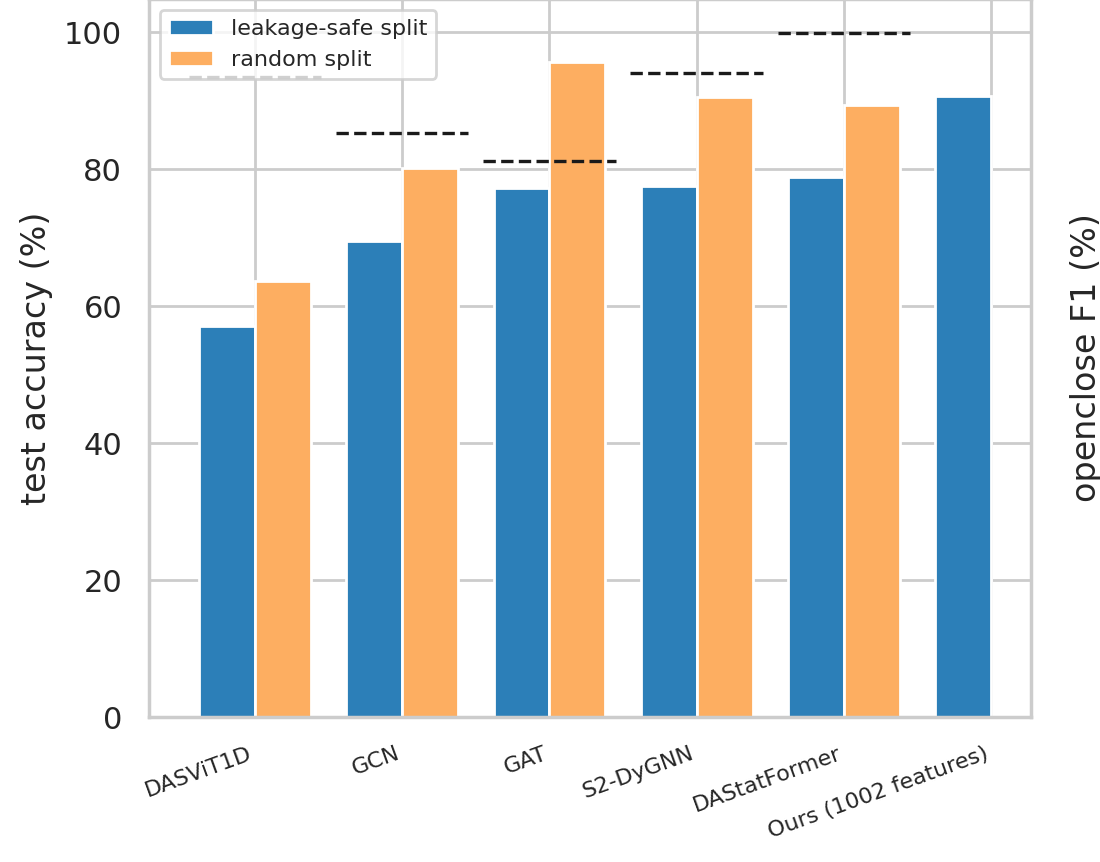
\includegraphics[width=\textwidth,keepaspectratio]{Figures/fig33a_sota_accuracy.png}
	\caption{Test accuracy under both partitions; dashed lines mark each method's published figure.}
\end{subfigure}\hfill
\begin{subfigure}[b]{0.48\textwidth}
	\centering
	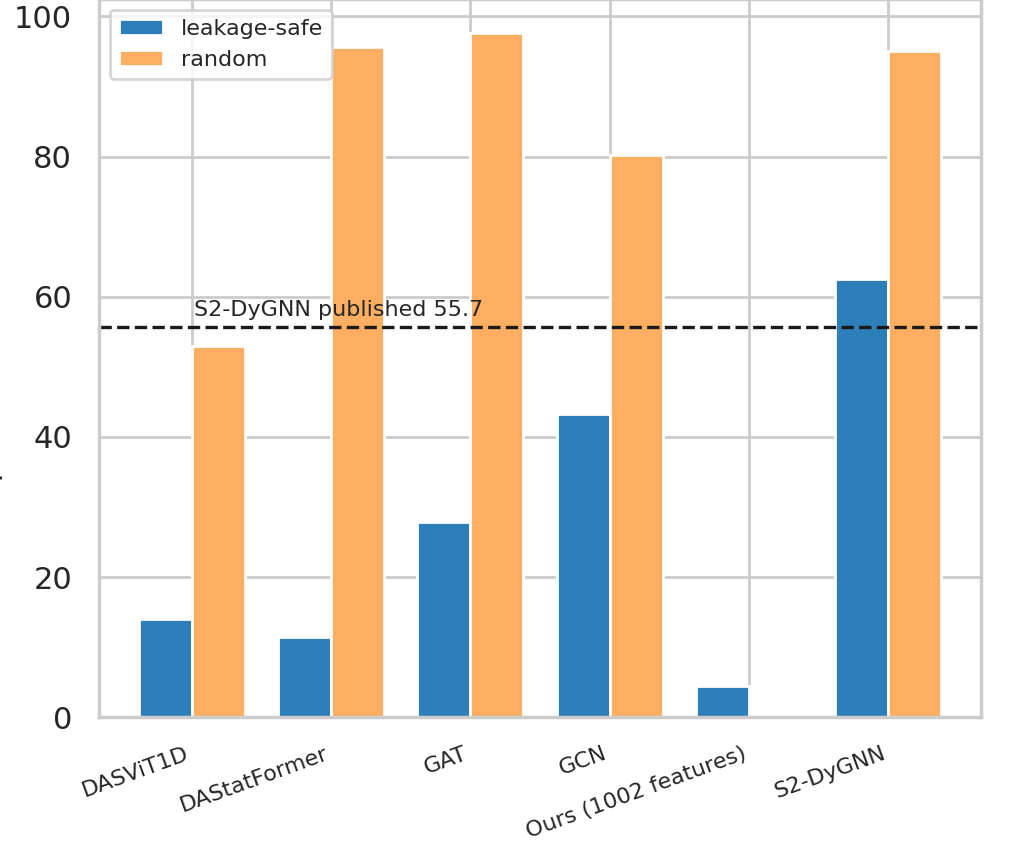
\includegraphics[width=\textwidth,keepaspectratio]{Figures/fig33b_sota_openclose.png}
	\caption{\emph{Openclose} $F_1$ under both partitions.}
\end{subfigure}\\[6pt]
\begin{subfigure}[b]{0.6\textwidth}
	\centering
	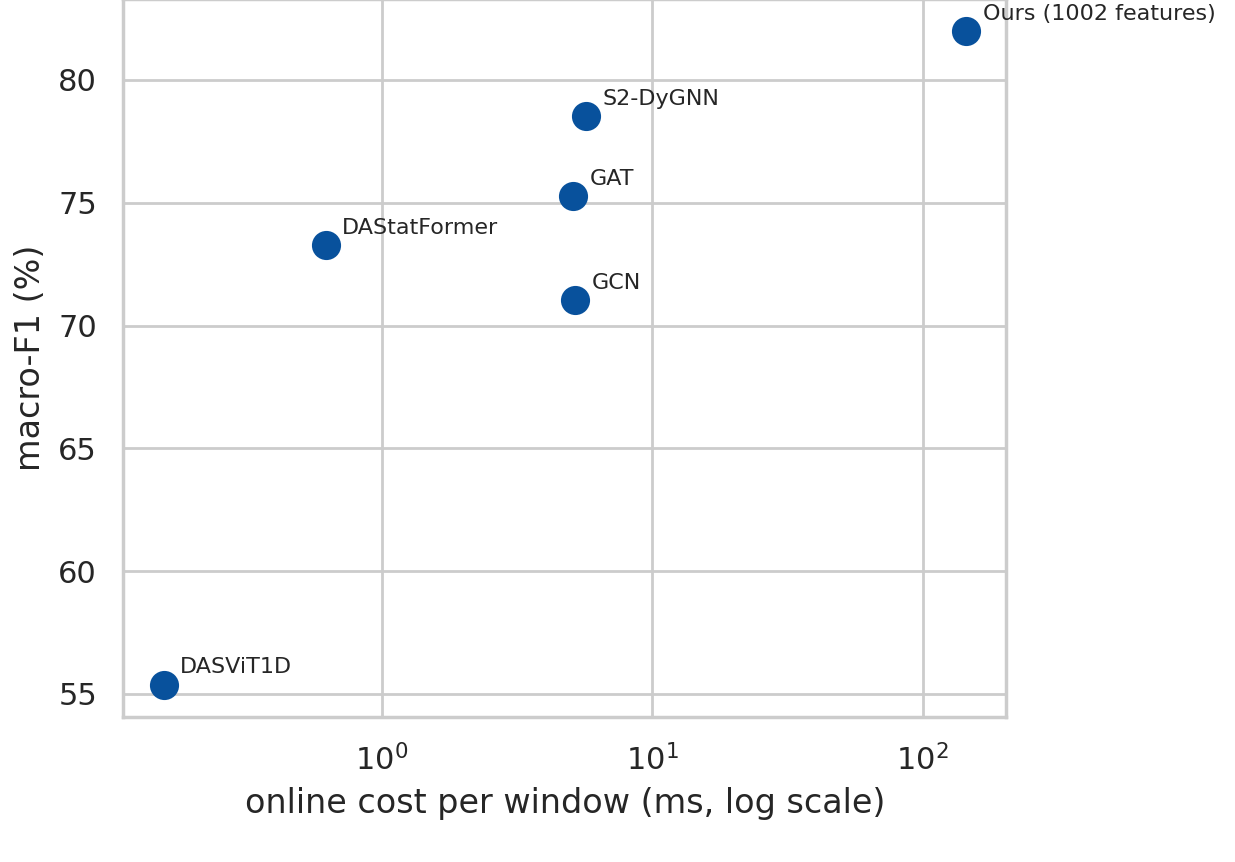
\includegraphics[width=\textwidth,keepaspectratio]{Figures/fig33c_sota_cost.png}
	\caption{Macro-$F_1$ against online cost per window (leakage-controlled partition).}
\end{subfigure}
\caption{Recent architectures against the feature pipeline on Tomasov, all trained on identical partitions. Online cost is measured on the Jetson AGX Orin and, for the feature pipeline, includes feature extraction.}
\label{fig:sota}
\end{figure}

Table~\ref{tab:sota_inflation} attributes the difference from the published figures. Each model was retrained on a random partition of the same windows, with only the partition changed, and every architecture gains on Tomasov: $18.38$ accuracy points for GAT, $13.01$ for S2-DyGNN, $10.62$ for GCN, $10.55$ for DAStatFormer, and $6.48$ for DASViT1D. On Cao, whose records are pre-segmented and non-overlapping, the same change alters accuracy by between $-6.24$ and $+2.03$ points with no consistent direction; the session contamination of the released Cao partition (\refs{sec:resLeakage}) inflates the released baselines but does not depend on window overlap. The effect is therefore a property of the protocol rather than of any architecture, and it is confined to the dataset whose windows overlap. This result reproduces, across five independent models, the single-model result of \refss{sec:resReproGap}. \reff{fig:protocol_inflation} shows the same two-arm comparison for every feature configuration of the pipeline itself: on Tomasov the full representation gains $6.8$ points under a random partition and every top-100 subset gains between $2$ and $7$, whereas on Cao no configuration changes by more than $2.1$.

\begin{table}[!htbp]
	\centering
	\caption{Protocol sensitivity of each architecture. The same model is retrained on a random partition of the same windows, changing only the partition. Values are test accuracy (\%).}
	\label{tab:sota_inflation}
	\small
	\resizebox{\textwidth}{!}{%
\begin{tabular}{@{}lrrrrrr@{}}
		\toprule
		\textbf{Model} & \textbf{Tomasov blocked} & \textbf{Tomasov random} & \textbf{$\Delta$} & \textbf{Cao grouped} & \textbf{Cao random} & \textbf{$\Delta$}\\
		\midrule
		GAT          & 77.33 & 95.70 & $+18.38$ & 96.28 & 98.32 & $+2.03$\\
		S2-DyGNN     & 77.59 & 90.60 & $+13.01$ & 84.14 & 82.18 & $-1.96$\\
		GCN          & 69.61 & 80.23 & $+10.62$ & 97.95 & 91.70 & $-6.24$\\
		DAStatFormer & 78.83 & 89.38 & $+10.55$ & 97.67 & 98.57 & $+0.90$\\
		DASViT1D     & 57.15 & 63.63 & $+6.48$  & 83.58 & 82.96 & $-0.63$\\
		\bottomrule
	\end{tabular}}
\end{table}

\begin{figure}[!htbp]
\centering
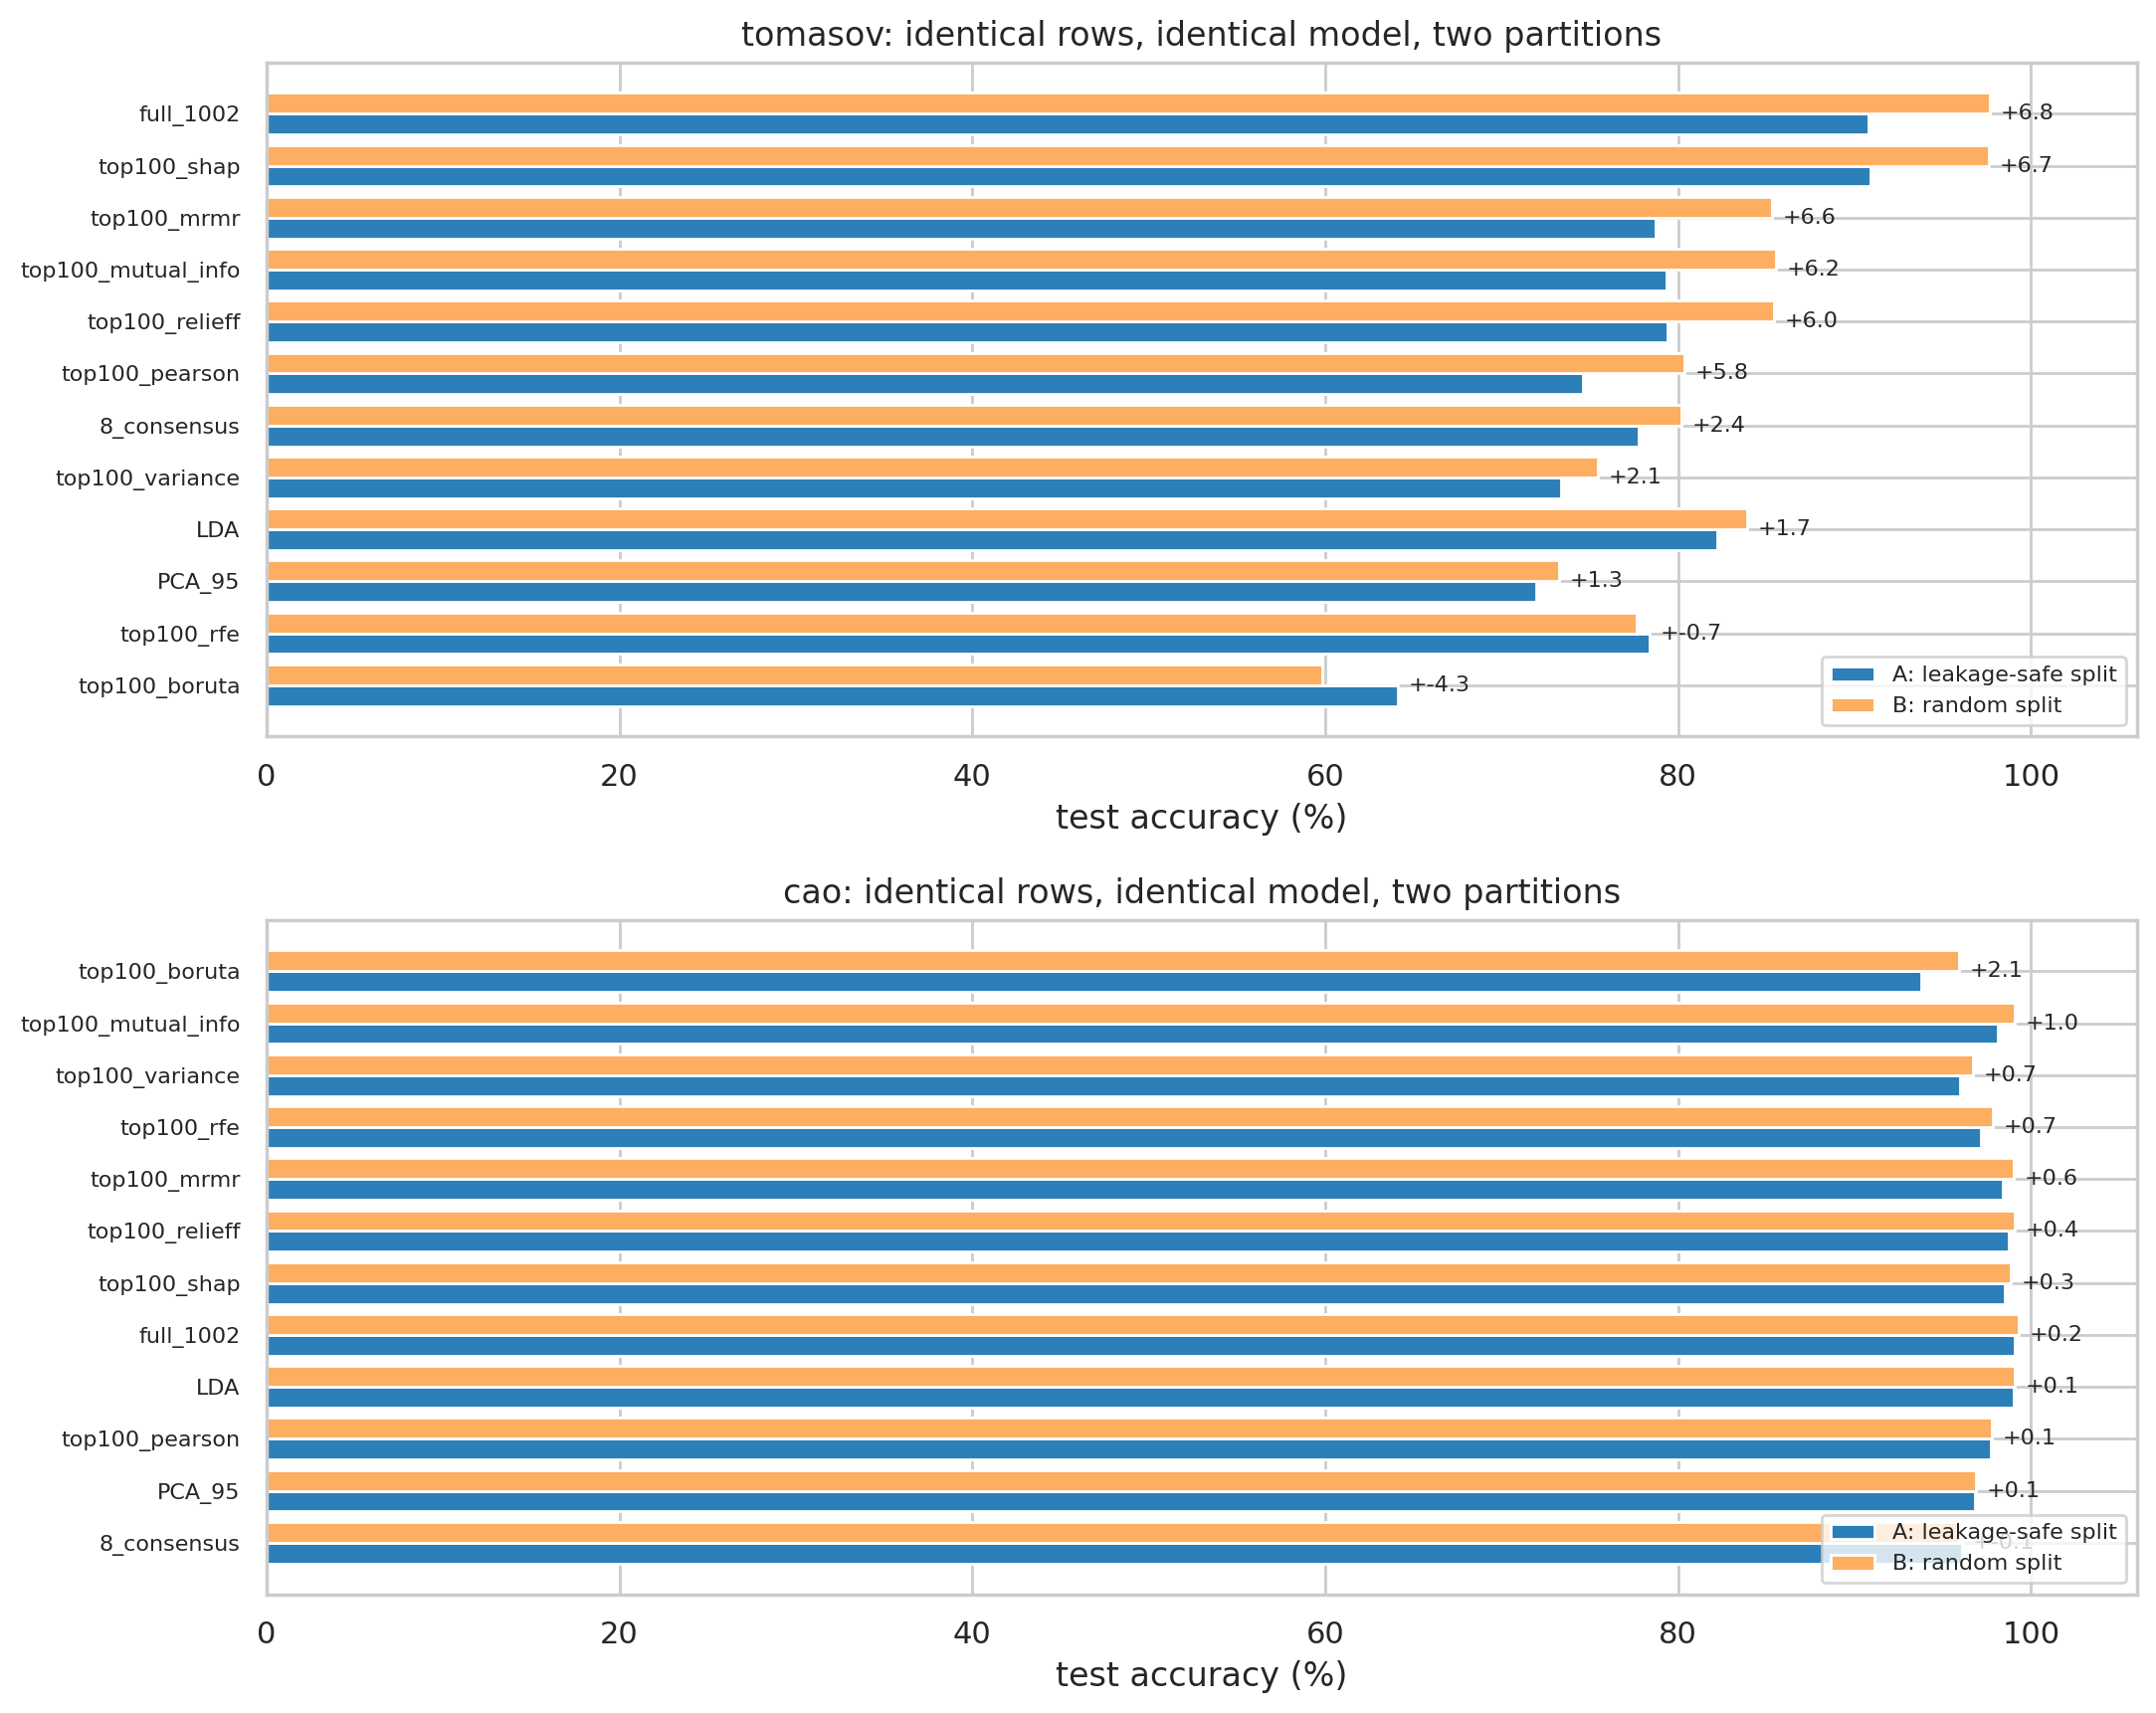
\includegraphics[width=0.88\textwidth,keepaspectratio]{Figures/fig34_protocol_inflation.png}
\caption{Protocol sensitivity of the feature pipeline: test accuracy of each feature configuration under the leakage-controlled and random partitions of the same rows, on Tomasov (top) and Cao (bottom). Annotations give the gain under the random partition.}
\label{fig:protocol_inflation}
\end{figure}

One result qualifies the overall advantage of the feature pipeline. As \refss{sec:resOpenclose} showed, no feature-based classifier recovers \emph{openclose} under leakage control ($F_1 = 0.044$ for the selected LightGBM and at most $0.189$ for any of the seven). S2-DyGNN achieves $0.625$ on the same partition and the same 198 test windows, exceeding the $0.557$ reported under its original protocol, and GCN reaches $0.433$. Models that operate directly on the channel axis thus recover a class that pooled spatial descriptors cannot distinguish.

A second qualification concerns cost, which Table~\ref{tab:sota} reports alongside the accuracies. The graph networks take preprocessed raw windows as input and compute their spectrograms within the network, so their online cost is their inference cost, $3.03$ to $5.67$\,ms per window on the GPU. DASViT1D and DAStatFormer read input features that are computed beforehand, which makes their $0.16$ to $0.76$\,ms a lower bound. The feature pipeline requires $144.59$\,ms of extraction on Tomasov and $122.54$\,ms on Cao before a classification that takes under $0.2$\,ms on the CPU. Per window and end to end, the networks are therefore faster online, and the smallest of them holds 48 thousand parameters. The lightweight advantages of the pipeline, presented in \refss{sec:resFootprint}, lie in a model a nineteenth the size of DAStatFormer and a tenth to a thirty-ninth that of the Tomasov CNN, sub-millisecond inference without a GPU, and training measured in minutes on CPU cores rather than hours on a GPU, and they are stated in those terms rather than as a lower latency.

\subsection{White-Box and Black-Box Models}
\label{sec:resWhiteBox}
\autoBookmark{subsec}{White-Box and Black-Box Models}
The preceding comparisons concern the performance of each model and its cost. This subsection addresses a different question: the extent to which a person can understand why a model reaches a given decision. It uses the distinction between white-box and black-box models introduced in \refss{sec:chap2AIMLDL}, and Table~\ref{tab:whitebox} places every model of the study on that scale. Logistic regression and the single decision tree are white boxes in the strict sense, since a weight or a threshold on a named descriptor constitutes the entire model. LightGBM, the selected learner, retains the property that is most important for audit, namely named inputs, but its $4{,}500$ trees on Tomasov are too numerous to be inspected individually. Its transparency therefore lies in its inputs, in its split structure, and in attributions that can be computed exactly for tree ensembles~\cite{lundberg2020trees}, and it is best described as a transparent ensemble over white-box features. The networks are black boxes. Their weights have no assigned meaning, and their decisions can be explained only retrospectively and only approximately~\cite{guidotti2018survey}. DAStatFormer is the closest to the pipeline, because its inputs are named statistics, but those statistics pass through 16 million weights of attention and gating layers before a decision is made.

\begin{table}[!htbp]
	\centering
	\caption{Interpretability of the models compared in this study.}
	\label{tab:whitebox}
	\footnotesize
	\setlength{\tabcolsep}{4pt}
	\renewcommand{\arraystretch}{1.15}
	\begin{tabularx}{\textwidth}{@{}>{\raggedright\arraybackslash}p{2.5cm} >{\raggedright\arraybackslash}X >{\raggedright\arraybackslash}X >{\raggedright\arraybackslash}X >{\raggedright\arraybackslash}p{1.75cm}@{}}
		\toprule
		\textbf{Model} & \textbf{Input} & \textbf{Meaning of a parameter} & \textbf{Explanation of a decision} & \textbf{Class}\\
		\midrule
		Logistic regression, decision tree & $1{,}002$ named descriptors & A weight or a threshold on one named descriptor & Read directly from the weights or the decision path & White box\\
		\addlinespace[3pt]
		LightGBM (proposed) & $1{,}002$ or 52 named descriptors, each tagged with its domain & A threshold on one named descriptor, or a leaf value & Exact Shapley attributions per window, split-based importance, and decision paths, all over named descriptors & Transparent ensemble\\
		\addlinespace[3pt]
		Tomasov and Cao CNNs & RDFT spectrum or raw record & A convolution or dense weight with no assigned meaning & Post-hoc saliency, approximate & Black box\\
		\addlinespace[3pt]
		DASViT1D & Vector of MFCC, RDFT, and DWT coefficients & A projection or attention weight & Post-hoc attention or saliency maps, approximate & Black box\\
		\addlinespace[3pt]
		DAStatFormer & 24 named statistics per channel & An attention or gating weight & Post-hoc and approximate; the inputs are named but mixed by attention & Black box\\
		\addlinespace[3pt]
		S2-DyGNN, GAT, GCN & Preprocessed multi-channel patch & A filter, graph, or attention weight; a learned channel adjacency & Post-hoc; learned edges show which channels interact, not why & Black box\\
		\bottomrule
	\end{tabularx}
\end{table}

The difference is not merely one of principle. In this thesis, interpretability enabled three analyses that would not have been possible with a black-box model. The first is the diagnosis of the spatial confound. Because every column carries its domain prefix, the representation could be decomposed domain by domain, and the leave-one-domain-out ablation and the recording-identity probe of \refs{sec:resConfound} showed that the 61 spatial descriptors both contribute $19.67$ macro-$F_1$ points and identify the source recording $11.1$ points beyond the next domain. For the networks, the same question, whether a model recognises the event or the recording, could be posed only externally, by changing the partition (\refss{sec:resReproGap}); it could not be traced to any part of the input.

The second is a comparison of the importance ranking with the definitions of the features. When the features are ranked by the frequency with which the final Tomasov model splits on them (\reff{fig:feature_importance}), five of its ten leading features, including the first three, are the Gini coefficient, maximum gradient, skewness, argmax, and kurtosis of the channel-energy profile. All five belong to the group of 29 descriptors that per-channel z-scoring makes constant in exact arithmetic (\refss{sec:chap3SpatialFeatures}). A model that relies most heavily on quantities that should carry no information is evidently using something other than the event, and the invariance audit of \refss{sec:chap5LimResidue} identified the source: a residue of approximately $10^{-14}$ left by a stabilising constant. Because each descriptor is an explicit formula, the audit could also identify the 33 descriptors that respond to changes that should not affect them. The learned features of a network have no definition against which such a check could be made.

The third is the interpretation of the selected subset. The unanimous subset is a short list of named quantities, and the five features selected on both systems, the minimum, lower quartile, and range of the STFT temporal envelope, the maximum spectral flux, and the Gini coefficient of the segment energies (\refss{sec:resConsistency}), describe how unevenly the energy of an event is distributed over the window and how abruptly its spectrum changes. An engineer can verify such statements against existing knowledge of the events, which is not possible for a learned embedding.

For perimeter security this property has practical as well as analytical value. An alert raised by the pipeline can be accompanied by the descriptors that produced it, so that an operator or an auditor can determine, for example, whether a fence alarm was based on impulsive time-domain structure or on the spatial distribution of the energy. Rudin~\cite{rudin2019stop} argues that in such high-stakes settings a model of this kind should be preferred to a black box explained retrospectively, because the explanation of a black box need not reflect the computation that the model performs. Exact attributions for tree ensembles avoid that discrepancy, since they are computed from the model itself rather than from a surrogate~\cite{lundberg2020trees}.

Interpretability is obtained at a cost, which the benchmark shows in two forms. Within the pipeline, the fully white-box learners are the weaker ones: on Tomasov the decision tree reaches $71.69$ and logistic regression $78.59$ macro-$F_1$, compared with $81.98$ for LightGBM, and on Cao $91.56$ and $97.84$ against $98.90$. The selected model therefore exchanges some transparency for accuracy. Relative to the networks, the cost is a loss of information. A designed representation retains only what its descriptors measure, and pooling over the channel axis discards the structure that enables S2-DyGNN to recover \emph{openclose} at an $F_1$ of $0.625$, whereas no feature-based learner exceeds $0.189$ (\refss{sec:resOpenclose}). The white-box design made that failure visible and explicable, but it did not prevent it. Nor has the benefit to operators been measured: the claim rests on named descriptors and attributions, and its evaluation with the personnel who act on alerts is reserved for future work (\refss{sec:chap5FutureOperators}).

On balance, the pipeline is more interpretable than the black-box networks in the sense that is relevant to audit: every input has a definition, every split refers to one of those inputs, and every attribution can be computed exactly. The same property enabled this thesis to identify, and to report, the most serious flaw in its own results.

\subsection{Overall Comparison with Published Work}
\label{sec:resSynthesis}
\autoBookmark{subsec}{Overall Comparison with Published Work}
Taken together, these comparisons explain why several results in this thesis are lower than those published for the same benchmarks. Every published Tomasov accuracy that could be re-measured under leakage control decreased: that of the reconstructed CNN from $85.47\%$ to $68.74\%$, and those of the five recent architectures by between $3.88$ and $36.35$ accuracy points, while the \emph{openclose} result of the first design cycle of this study decreased from an $F_1$ of $0.72$ to $0.044$. The controlled two-arm comparisons attribute a large proportion of these reductions to the evaluation protocol rather than to the reimplementations, since changing only the partition of otherwise identical models raises the accuracy of the reconstructed CNN by up to $26.27$ points and that of the five architectures by between $6.48$ and $18.38$ points. On Cao, whose records do not overlap, the same intervention has no consistent effect, which confines the inflation to the dataset whose windows overlap. Published figures on the Tomasov benchmark therefore cannot be compared with one another, or with leakage-controlled results, until the protocol underlying each is taken into account.

The relative standing of the methods also changes. Under their own protocols, DAStatFormer and S2-DyGNN report the highest accuracies on the Tomasov benchmark, yet under identical leakage-controlled partitions the feature pipeline exceeds them by $11.88$ and $13.12$ accuracy points, although the graph models retain their lead on \emph{openclose}. Leakage does not inflate all models equally: the low-capacity Cao CNN lost only $1.58$ accuracy points when its released partition was replaced by the session-grouped partition, whereas the graph and transformer models gained between $6.48$ and $18.38$ points from a random partition of the same Tomasov windows. Rankings obtained under contaminated protocols therefore need not agree with rankings obtained under group-aware evaluation, and for this reason every comparison in this thesis is made on identical partitions. These conclusions concern generalisation to unseen segments of represented recordings. As \refs{sec:resGeneralisationAll} and \refs{sec:resMapping} showed, performance declines further when whole recordings or acquisition campaigns are held out and collapses when a fitted model is transferred to another sensing system, regimes that none of the studies reviewed in \refs{sec:chap2RelatedWorks} evaluates.

Three of these measurements have no counterpart in the reviewed studies and constitute the principal additions of this thesis to the DAS literature: the attribution of a reproduction gap to the protocol by changing only the partition, the recording-identity probe that measures how much information each feature domain carries about the acquisition, and the transfer of a fitted model between two independent sensing systems over a mapped taxonomy. With these comparisons, \textbf{RQ3} is answered: the pipeline outperforms the published and recent baselines on identical partitions while remaining lightweight in model size, training cost, and hardware, and transparent where the networks are black boxes. It does so at a known cost in end-to-end latency, with known limits on the transferability of a fitted model, and, on Tomasov, with a margin that depends on the numerical residue of \refss{sec:chap5LimResidue}.

\section{Summary}%
\label{sec:chap4Summary}
\autoBookmark{sec}{Summary}
This chapter evaluated the artefact on the primary Tomasov dataset and the Cao evaluation dataset under a verified leakage-controlled protocol. The audit that established that protocol found that every Tomasov test window shared raw samples with a training window under a random split and that 423 of 441 Cao sessions spanned the published partition; blocked, guard-banded and session-grouped partitions reduced both measures to zero.

For \textbf{RQ1}, the footprint of every model was measured on the Jetson AGX Orin. The selected LightGBM holds $855{,}000$ parameters ($3.42$\,MB) on Tomasov and $208{,}578$ ($0.83$\,MB) on Cao, trains in $1{,}357$ and $41$\,s on CPU cores, and classifies a window in $0.17$ and $0.06$\,ms without a GPU. The model is thus a nineteenth the size of DAStatFormer and about a tenth that of the smaller Tomasov CNN, and its training requires no GPU, whereas the graph networks require seven to ten and a half hours of GPU training on Tomasov. The graph networks are smaller still and less costly end to end, because feature extraction ($122.54$--$144.59$\,ms per window) dominates the online cost of the pipeline; that cost fits within the window-arrival interval on one CPU core for Cao and two for Tomasov. The pipeline is therefore lightweight in its learning stage and its hardware requirements, and feature extraction is its most expensive component.

For \textbf{RQ2}, fusion outperformed every individual domain by $6.26$ macro-$F_1$ points on Tomasov and $3.46$ on Cao; unanimous eight-method consensus reduced the feature space by approximately $95\%$ and the training time by factors of $5.3$ to $21.5$, at a cost of $8.39$ and $5.81$ points and without reducing the size of the fitted model; and the six balancing strategies could be distinguished only modestly on Tomasov and not at all on Cao. The three gradient-boosting learners led all seven classifiers and lay within $0.62$ and $0.84$ macro-$F_1$ points of one another, and LightGBM, which validation selected in every configuration, is therefore best regarded as the representative of that tier. The pipeline designed on Tomasov was applied unchanged to Cao.

For \textbf{RQ3}, the selected configuration exceeded the CNN published with each dataset by $16.43$ and $8.01$ macro-$F_1$ points and exceeded five architectures published from 2024 onwards on identical partitions, although channel-level graph models recover \emph{openclose} where the pipeline does not. Changing only the partition altered the accuracy of an otherwise identical CNN by $26.27$ points, every recent architecture gained between $6.5$ and $18.4$ points under a random split, and removing the leakage reduced the \emph{openclose} $F_1$ of the selected model from $0.72$ to $0.044$. Unlike the black-box networks, the pipeline reaches its decisions through named descriptors, which enabled the spatial confound and the numerical residue to be traced. Generalisation beyond represented recordings is weaker. Spatial descriptors identified the source recording $11.1$ points above the next domain while contributing $19.67$ macro-$F_1$ points, two effects that this dataset cannot separate; leave-one-recording-out accuracy on Tomasov averaged $63.85\%$; holding out Cao acquisition dates reduced accuracy from $99.06\%$ to $86.81\%$; and although four event types could be mapped between the two taxonomies, a model trained on one system performed below chance on the other. Chapter~\ref{chap:Conclusion} consolidates these findings, states their novelty, and reports a numerical residue in the normalisation that qualifies the Tomasov figures.
